
\documentclass[11pt, review]{elsarticle} % first argument is font-size for document
\graphicspath{ {./images/} }
\usepackage{hyperref}
\usepackage{float}
\usepackage{verbatim} %comments
\usepackage{apalike}


%custom:
\usepackage{mathastext}
\usepackage{pgfplots}
\pgfplotsset{width=7cm,compat=1.8}
\definecolor{custombeige}{HTML}{e0d4ba}
\definecolor{custombeigeouter}{HTML}{968f7e}
\definecolor{customgray}{HTML}{666666}
\definecolor{customgrayouter}{HTML}{404040}

\usepackage % Sets margin distance left and right
[
        left=3.5cm,
        right=3.5cm,
]
{geometry}

\usepackage{caption}
\captionsetup{font=footnotesize}

\usepackage{subfigure}

\usepackage{xcolor}
\usepackage{soul}

\usepackage[bordercolor=white,backgroundcolor=gray!30,linecolor=black,colorinlistoftodos]{todonotes}
\newcommand{\hlc}[1]{\todo[color=yellow,inline]{#1}}



\restylefloat{figure}
\restylefloat{table}

\journal{Expert Systems with Applications}

\bibliographystyle{model5-names}\biboptions{authoryear}

% Fixes row-to-row distance
\renewcommand{\baselinestretch}{1.0}

\begin{document}
\begin{frontmatter}


\begin{titlepage}
\begin{center}
\vspace*{1cm}

\textbf{ \large Detecting ditches using supervised learning on high-resolution digital elevation models}

\vspace{1.5cm}

Jonatan Flyckt$^{a}$ (fljo1589@student.ju.se), Filip Andersson$^{a}$ (anfi1632@student.ju.se), Niklas Lavesson$^a$ (niklas.lavesson@ju.se), Liselott Nilsson$^b$ (liselott.nilsson@skogsstyrelsen.se), Anneli M. \AA gren$^c$ (anneli.agren@slu.se) \\

\hspace{10pt}

\begin{flushleft}
\small  
$^a$ J\"onk\"oping Artificial Intelligence Laboratory, J\"onk\"oping University, Gjuterigatan 5, 551 11, J\"onk\"oping, Sweden \\
$^b$ Forest Department, Swedish Forest Agency, Skeppargatan 17, 931 32 Skellefte\aa, Sweden \\
$^c$ Department of Forest Ecology and Management, Swedish University of Agricultural Sciences, SLU, Skogsmarksgr\"and 17, 901 83, Ume\aa, Sweden

\begin{comment}
Clearly indicate who will handle correspondence at all stages of refereeing and publication, also post-publication. Ensure that phone numbers (with country and area code) are provided in addition to the e-mail address and the complete postal address. Contact details must be kept up to date by the corresponding author.
\end{comment}

\vspace{1cm}
\textbf{Corresponding Author:} \\
Niklas Lavesson \\
J\"onk\"oping Artificial Intelligence Laboratory, J\"onk\"oping University, Gjuterigatan 5, 551 11, J\"onk\"oping, Sweden \\
Tel: (+46) 70-5383338 \hl{Ska detta nummer st\aa  h\"ar? (corresponding author m\aa ste ha telefonnummer)} \\
Email: niklas.lavesson@ju.se

\end{flushleft}        
\end{center}
\end{titlepage}

\title{Detecting ditches using supervised learning on high-resolution digital elevation models}

\author[ju]{Jonatan Flyckt\corref{equal_contribution}}
\ead{fljo1589@student.ju.se}

\author[ju]{Filip Andersson\corref{equal_contribution}}
\ead{anfi1632@student.ju.se}

\author[ju]{Niklas Lavesson\corref{cor1}}
\ead{niklas.lavesson@ju.se}

\author[fa]{Liselott Nilsson}
\ead{liselott.nilsson@skogsstyrelsen.se}

\author[slu]{Anneli M. \AA gren}
\ead{anneli.agren@slu.se}

\cortext[cor1]{Corresponding author.}
\address[ju]{J\"onk\"oping Artificial Intelligence Laboratory, J\"onk\"oping University, Gjuterigatan 5, 551 11, J\"onk\"oping, Sweden}
\address[fa]{Forest Department, Swedish Forest Agency, Skeppargatan 17, 931 32 Skellefte\aa, Sweden}
\address[slu]{Department of Forest Ecology and Management, Swedish University of Agricultural Sciences, SLU, Skogsmarksgr\"and 17, 901 83, Ume\aa, Sweden}
\cortext[equal_contribution]{Jonatan Flyckt and Filip Andersson contributed equally to this work as first authors.}

\begin{abstract}
{\footnotesize
Drained wetlands can constitute a large source of greenhouse gas emissions, but the drainage networks in these wetlands are largely unmapped, and better maps are needed to aid in forest production and to better understand the climate consequences. We develop a method for detecting ditches in high resolution digital elevation models derived from LiDAR scans. Thresholding methods using digital terrain indices can be used to detect ditches, however, a single threshold generally does not capture the variability in the landscape, and generates many false positives and negatives. We hypothesise that, by combining the digital terrain indices using supervised learning, we can improve ditch detection at a landscape-scale. In addition to digital terrain indices, additional features are generated by transforming the data to include neighbouring cells for better ditch predictions. A Random Forests classifier is used to locate the ditches, and its probability output is processed to remove noise, and binarised to produce the final ditch prediction. The confidence interval for the Cohen's Kappa index ranges \textbf{[0.655 , 0.781]} between the evaluation plots with a confidence level of \textbf{95\%}. The study demonstrates that combining information from  a suite of digital terrain indices using machine learning provides an effective technique for automatic ditch detection at a landscape-scale, aiding in both practical forest management and in combatting climate change.}
\end{abstract}

\begin{keyword}
{\footnotesize
Machine learning \sep Geographic information systems \sep Classification and regression trees \sep Supervised learning by classification}
\end{keyword}

\end{frontmatter}

\newpage
\section{Introduction}\label{introduction}

Over the last century, the wetlands in North Europe and parts of North America have been substantially modified and ditched. In many places both the landscape and the channel network have also been heavily altered  by humans, especially in the agricultural landscapes, for example in mid-western United States \citep{passalacqua}. In North Europe, however, ditches have mainly been dug to turn flat peatlands into productive forests, resulting in profound impacts on the hydrology of this region. \citep{peatlands}. In Sweden, which is one of the North European countries with the most extensive ditch network, over five million hectares of peatland have been drained for forestry in the 20th century.  As a result, almost one million km of ditches have been introduced, which has doubled the length of watercourses across Sweden  \citep{hasselquist}.

The forest industry and agencies have a demand for better maps of the ditch networks in the forest landscape. Drained afforested peatlands contribute strongly to Swedish wood production, and consequently to the Swedish economy. At the same time, Swedish authorities have identified drained wetlands as a major target for greenhouse gas mitigation \citep{greenhouse_skogsstyrelsen, greenhouse_jordbruksverket}. However, research on the effects of afforested drained wetlands on greenhouse gas emission is inconclusive, and they can constitute both a source and a sink for greenhouse gases \citep{greenhouse_yes, greenhouse_no}. There is a need for science-based tools to optimise both forest production and decision support systems for mitigation of greenhouse gas emissions from drained forested wetlands. A key step to accomplish this is to map the ditch networks in the forest landscape. However, it is unfeasible to conduct landscape-scale field inventories, as they are often both challenging and expensive.

The National Inventory of Landscapes in Sweden (NILS) has recorded small watercourses (width $<$ 6 m) by conducting a line inventory in 631 $5*5$ km squares randomly distributed in Sweden, to best capture a representative and varied sample of the Swedish landscape. The positions of the small watercourses from this inventory were compared with the watercourses on Swedish Property Map (1: 12 500) (\hyperref[fig:watercoursebarplot]{Figure} \ref{fig:watercoursebarplot}). A total of 1103 natural watercourses, 131 straightened watercourses/channels, and 2089 ditches were found in the field. This simple investigation highlights two things: First, ditches make up the majority of the small scale water channels in the Swedish landscape; almost twice as many as the natural streams. Second, most of the small scale channels are missing on the current maps; only 45 \% of the natural watercourses, 25 \% of the straightened watercourses/channels, and 9 \% of the ditches are mapped (\hyperref[fig:watercoursebarplot]{Figure} \ref{fig:watercoursebarplot}).

\begin{figure}[!htb]
    \centering
    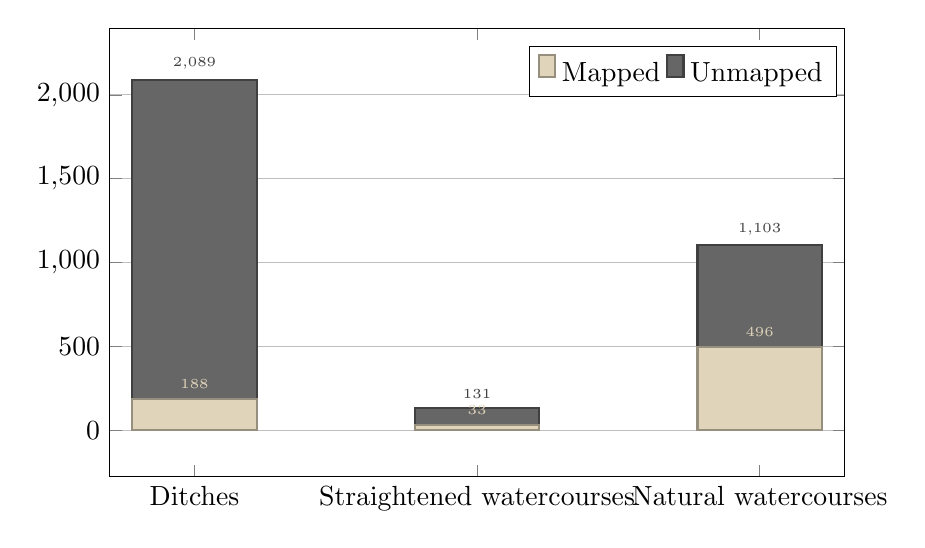
\begin{tikzpicture}
    \begin{axis}[
        width={0.9\textwidth},
        height={0.6\textwidth},
        ylabel={fluorescence},
        ybar stacked,
        ymajorgrids=true,
    	bar width=45pt,
    	nodes near coords,
    	every node near coord/.append style={font=\tiny},
        enlarge y limits={0.15},
        enlarge x limits=0.15,
        legend style={at={(0.78,0.96)},
          anchor=north,legend columns=-1},
        ylabel={{}},
        symbolic x coords={Ditches, Straightened  watercourses, Natural  watercourses},
        xtick=data,
        ytick={0,500,1000,1500,2000},
        x tick label style={rotate=0,anchor=north},
        ]
    \addplot+[ybar,color=custombeige,fill=custombeige,draw=custombeigeouter,thick] plot coordinates {(Ditches,188) (Straightened  watercourses,33) 
      (Natural  watercourses,496)};
    \addplot+[ybar,color=customgrayouter,fill=customgray,draw=customgrayouter,thick] plot coordinates {(Ditches,1901) (Straightened  watercourses,98) 
      (Natural  watercourses,607)};
    \legend{\strut Mapped, \strut Unmapped}
    \end{axis}
    \end{tikzpicture}
    \caption{\textbf{Channel mapping status.} The bars indicate the number of observed channels in the National Inventory of Landscapes in Sweden's (NILS) line inventory of small watercourses (width $<$ 6 m). The colours of the bars indicate whether they are mapped or not on the Swedish Property map.}
    \label{fig:watercoursebarplot}
\end{figure}

Several previous studies have located ditches from remote sensing Light Detection and Ranging (LiDAR) data in smaller agricultural areas \citep{roelens, bailly} or smaller forest areas (smaller than 2 $km^2$) \citep{rapinel, kiss}, predominantly characterised by artificial drainage. In this study, however, we conduct a landscape-scale analysis in a mesoscale catchment. The study  catchment  is 68 $km^2$, representing diverse landscape features and geomorphological characteristics. Additionally, the forest landscape introduces many challenges that are not present when detecting ditches along roads or in agricultural areas. The canopy cover in forest areas prevents the use of satellite imagery or aerial photos, as well as lowers the quality of the digital elevation models (DEMs), as fewer LiDAR points reach the ground, instead frequently catching in trees, bushes, or grass. Forest ditches are also generally not maintained to the same extent as agricultural or road ditches, often being overgrown or covered by windthrows or windsnaps. Using raw LiDAR point clouds to detect ditches, as \citet{roelens} and \citet{bailly} did in their studies can thus be problematic in a forest landscape, where a DEM constructed to map the points on the ground should be more suitable. \citet{cazorzi} used a DEM with image processing techniques aimed at detecting the elongated ditch shapes and excluding large landscape features. This approach worked well for their open agricultural areas, but is difficult to generalise to a diverse forest landscape. Instead, we will focus on the topographical incision of the ditches in the DEM, which will be highlighted with a set of digital terrain indices. Previous studies have found that terrain indices such as \hyperref[skyviewfactor]{Sky View Factor} \citep{zaksek}, \hyperref[impoundment]{Impoundment Index} \citep{whiteboxtools} and High Pass Median Filter \citep{whiteboxtools} can detect ditches in forest landscapes in some cases \citep{uppsala}. However, different false positives and negatives can be observed when examining each terrain index manually. These inaccuracies can stem either from the gaps in the LiDAR scans, or from a poorly set threshold for the terrain index parameters. Thus, it would be useful to combine these terrain indices to prune the weaknesses and amplify the strengths of each index to produce a highly accurate detection of ditch networks. 

In this study, we introduce a new method for the automated mapping of ditches by integrating multiple high resolution terrain indices using a supervised learning approach. Several features and post-processing steps, specifically tailored for ditch detection are also developed and employed. These features aim to both highlight elongated shapes similarly to \citet{cazorzi}, as well as include a map of the neighbouring area as \citet{roelens} did in their study. We hypothesise that by combining the information from all the digital terrain indices using a machine learner (Random Forests), we can improve the detection of the ditches, compared to if a single terrain index is used. To test this, we conduct a landscape-scale ditch detection analysis at the Krycklan Catchment in Sweden \citep{krycklancatchment}, where a high precision manual ditch mapping has been performed. This manual mapping guided the model training and ground-truthing in our analysis and provided a test-bench for our methodology.

\section{Materials and method}
\label{method}

\subsection{Study area and dataset}
The quaternary deposits in the Krycklan Study Catchment are dominated by till (51\%) and sorted sediments (30\%). The catchment ranges in elevation from 114 to 405 m above sea level. Forest covers 87\% of the catchment, mires 9\%, thin soils 7\%, and rock outcrops 1\%. The land use is dominated by forestry; approximately 25\% of the Krycklan catchment has been protected since 1922, but  the rest of the area is mostly second growth forest \citep{krycklancatchment}.  A historical survey of the catchment (Gudrun Norstedt, unpublished) recorded  that the ditches in the catchment were dug between 1900 and 1993. Initially, the ditches were dug to drain the mires for hay production. Later on, wet areas were drained to attempt to turn them into productive forest lands \citep{paivanen}. However, research later showed that many of the drained mires were not productive for forestry due to lack of nutrients \citep{sikstrom}.

The LiDAR dataset used in this study was produced by TerraTec Sweden AB in August 2015, on demand of the Department of Forest Resource Management at the Swedish University of Agricultural Sciences, and is freely available online \citep{dataset}. The average density of the dataset is 20 pulses per $m^2$. Ground point classification was performed with lasground (included in LAStools, a software suite produced by rapidlasso GmbH). The DEM was created with blast2dem (included in LAStools), with a cell size of $0.5*0.5$ m. Only ground points were imported to generate a DEM of the ground.

\subsection{Digitising the ground truth}
For training and validation, a vector layer of all ditches in the Krycklan Catchment \citep{krycklancatchment} was digitised. The study catchment comprises several types of ditches including road ditches, forest ditches, and agricultural ditches. A multidirectional hillshade of the 0.5 m DEM was calculated in ArcGIS Pro, and from this layer, most of the ditches could be easily identified by a human. We conducted the digitisation at a scale of 1:600 to ensure that all the digitised ditches are properly aligned with the actual ditch on the ground, and do not coincide with the edge of the banks. In addition, both current and historical records and orthophotos dating back to the 1960's were consulted to help locate all the ditches. In uncertain areas, the ditches were verified in the field. The digitisation of the ditch networks showed that there are 107 km of road ditches and 208 km of forest/agricultural ditches in the catchment (\hyperref[fig:swedenkrycklan]{Figure} \ref{fig:swedenkrycklan}). The stream network in \hyperref[fig:swedenkrycklan]{Figure} \ref{fig:swedenkrycklan} shows a 197 km long network with a 8 hectare flow initiation threshold, representing median flow conditions.

\begin{figure}[!htb]
    \centering
    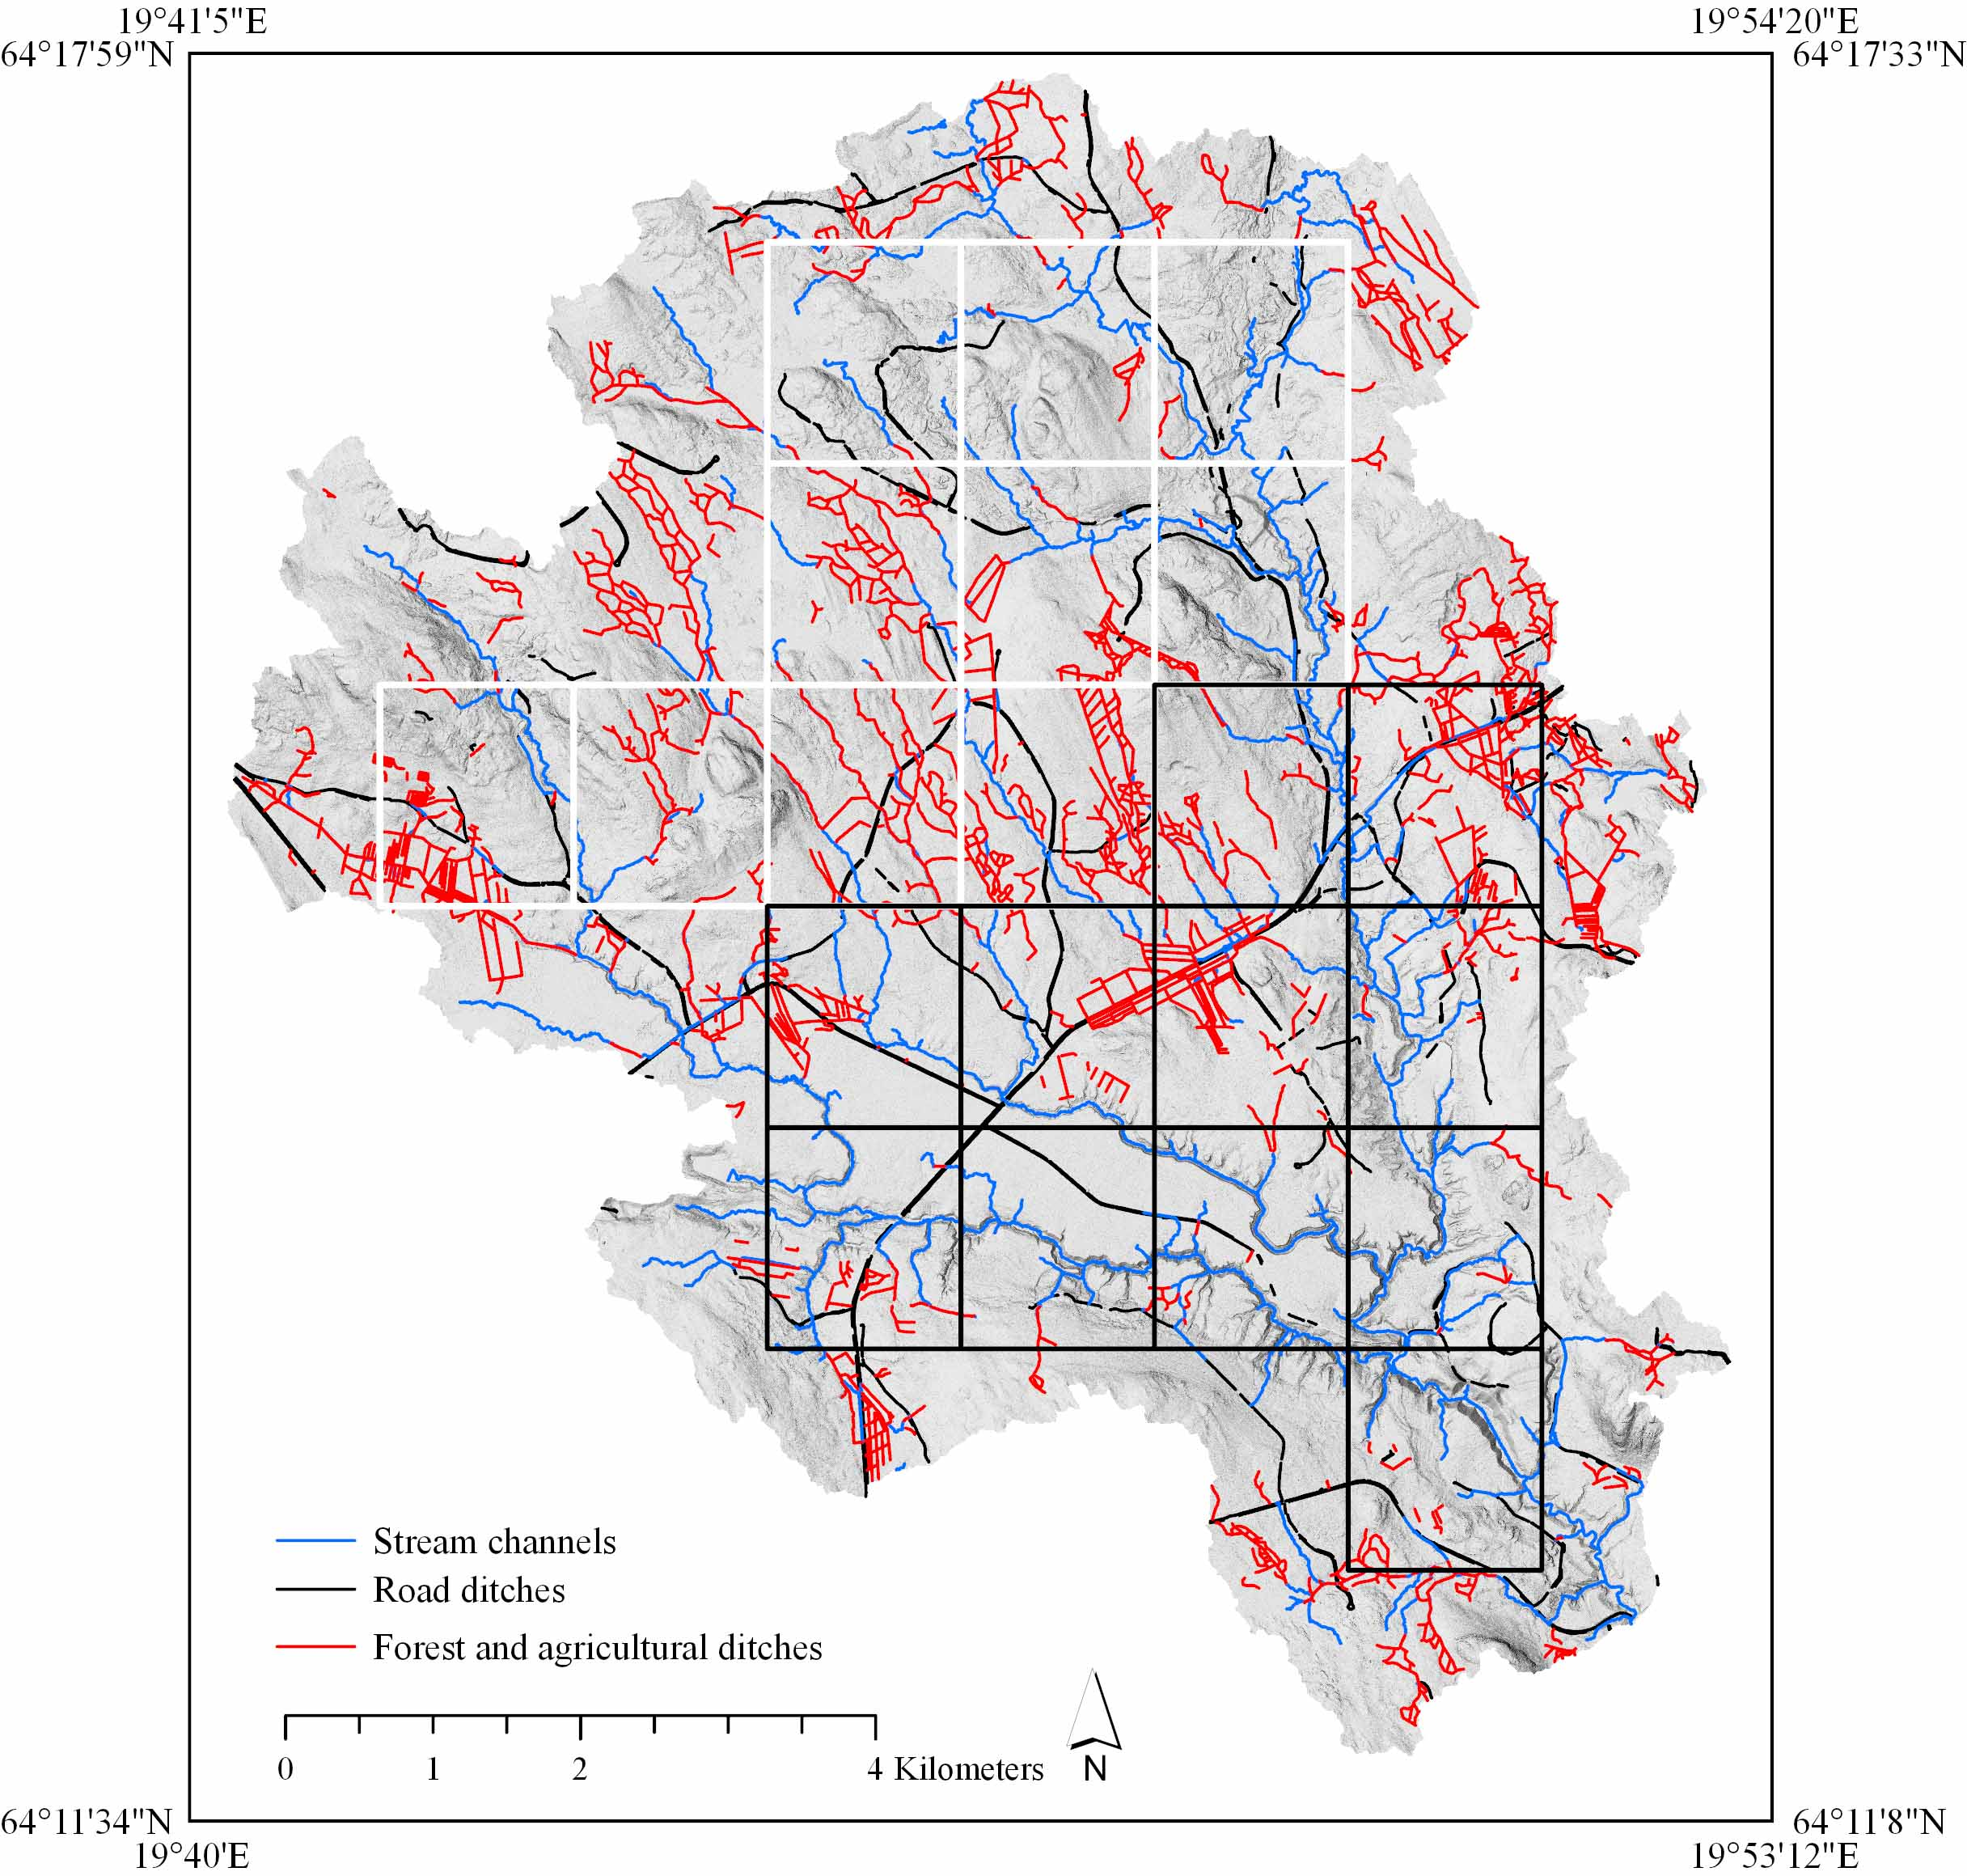
\includegraphics[width=1\linewidth]{./images/Krycklan_lo.jpg}
    \caption{\textbf{Krycklan channel map.} Shows ditches and stream channels in the Krycklan catchment, as well as our division into 21 subsections of $2997 \cdot 2620$ pixels (roughly 196 hectare each). The 10 subsections with a white border were used for developing features and optimising parameters before the experiment. The 11 subsections with a black border were used in the experiment for evaluation with 11-fold cross validation.}
    \label{fig:swedenkrycklan}
\end{figure}

From the ditch mapping, the vector layer was rasterised with a resolution of $0.5*0.5$ metres for use as a ground-truth for our ditch detector. Our field observations have shown that most of the ditches in the catchment range between 0.5 and 3.5 metres in width. To ensure that all ditch pixels were labelled correctly for the model in the training phase, we labelled all pixels within three pixels (1.5 metres) of the vectors as ditch pixels, making the labels 3.5 metres wide (\hyperref[fig:ditchpreprocess]{Figure} \ref{fig:ditchpreprocess}). Due to all ditches varying in width, it was impossible to produce a perfect representation of each ditch, but this widening helped ensure that almost all ditch pixels were covered by the labels. To match the labels with our predictions (where we downscale the predictions into grids to remove outliers), the ground-truth was also downscaled into grids of $6*6$ pixels (9 $m^2$) each by labelling each grid cell containing at least 25\% ditch pixels as a ditch (\hyperref[fig:ditchpreprocess]{Figure} \ref{fig:ditchpreprocess} \hyperref[fig:ditchpreprocess]{c}).

\begin{figure} [!htb]
    \centering
    \subfigure[]{
        \resizebox*{3.5cm}{!}{\includegraphics{./images/publ_ditch_preprocess_A_lo.jpg}}}\hspace{5pt}
    \subfigure[]{
        \resizebox*{3.5cm}{!}{\includegraphics{./images/publ_ditch_preprocess_B_lo.jpg}}}
    \subfigure[]{
        \resizebox*{3.5cm}{!}{\includegraphics{./images/publ_ditch_preprocess_C_lo.jpg}}}
    \caption{\textbf{Processing of ditch labels.} \textbf{a: }Rasterised ditches with a width of one pixel. \textbf{b: }Ditches after a widening process, seven pixels (3.5 metres) wide. Used as labels when training the models. \textbf{c: }Ditches after a grid zone conversion. Used for evaluating the results from the ditch detector.} \label{sample-figure}
    \label{fig:ditchpreprocess}
\end{figure}

\subsection{Extracting ditches with digital terrain indices}
From the DEM, several digital terrain indices were calculated:
\begin{itemize} \label{data_attributes}

  \item \textbf{Sky View Factor} \label{skyviewfactor} \newline
    The Sky View Factor represents how much of the sky that is visible from a certain point on the ground \citep{zaksek}. A point inside a ditch would produce a low value, as more of the sky is obscured by the ditch bank. Sky View Factor tends to produce false positives in steep terrain. The index was calculated in SAGA GIS, using a search radius of 10 metres to ensure that it was large enough to capture the ditches, but small enough to not include large scale topographical features such as hills.

  \item \textbf{Impoundment Index} \label{impoundment} \newline
    The Impoundment Index in Whitebox Tools \citep{whiteboxtools} can be used as a measure of flow constriction, which is useful for mapping channels such as ditches. When tuned to output the flooded volume, it effectively maps the area and average depth of the reservoir that would be created by placing a dam of a user-specified length at each grid cell in the DEM. Here, we used dam height calculated with a dam length of 3 metres to attempt to cover the entire ditches. Typical false positives with this index are natural stream channels with a clear incised channel.
  
  \item \textbf{High Pass Median Filter} \label{hpmf} \newline
    High Pass Median Filters (HPMF) highlight ditches by indicating local depressions (such as ditches) in the DEM by subtracting the value at the grid cell at the centre of the window from the median value in the window. Typical false positives with this index are small hollows. HPMF was calculated using Whitebox Tools \citep{whiteboxtools} with a window size of $4.5 * 4.5$ m. 

    \item \textbf{Slope} \label{slope} \newline
    The Slope index represents the degree of slope at a certain point, with a value ranging from $0^{\circ}$ to $90^{\circ}$ with no information about the direction of the slope. It was calculated on the 0.5 m grid, using ArcGIS \citep{EsriArcGisBook}.
\end{itemize}

To benchmark our method against a non-machine learning method, we binarised the original four digital terrain indices using thresholds. Different threshold values were tested and the value that yielded the highest Cohen's Kappa score for each respective index was chosen. This test was conducted for the 11 subsections described in \hyperref[trainingvalidationdatasets]{section} \ref{trainingvalidationdatasets}. \hyperref[skyviewfactor]{Sky View Factor} was classified to only include values below 0.955, the \hyperref[impoundment]{Impoundment Index} Dam Height using values above 0.27 $m$, \hyperref[hpmf]{HPMF} using values below -0.18 m, and the \hyperref[slope]{Slope} index using values above $14 ^{\circ}$ (\autoref{recreatedpredictionperformance}).

\subsection{Data preparation}

\subsubsection{Feature engineering}

The digital terrain indices provided a satisfactory foundation for the models, but could not always generalise well to outlier situations. To give a representation of the area surrounding a specific pixel, we extracted more diverse features using simple statistical aggregates such as mean, median, min, max, and standard deviation in different circular radii around the pixel (similar to the approach of \citet{roelens}). This aided in pruning pixels with outlier values, often smoothing out the data to represent ditches more accurately on a per-pixel basis (\hyperref[fig:features]{Figure} \ref{fig:features}: \hyperref[fig:features]{b}, \hyperref[fig:features]{c}, \hyperref[fig:features]{f}, and \hyperref[fig:features]{g}). Additionally, several features were generated by using thresholds on one or multiple indices to exclude, lower, or amplify the values of pixels that indicated ditches or non-ditches (\hyperref[fig:features]{Figure} \ref{fig:features}: \hyperref[fig:features]{d} and \hyperref[fig:features]{h}).

Features were generated for both \hyperref[hpmf]{HPMF} and \hyperref[skyviewfactor]{Sky View Factor} using the image processing \textit{gabor filter}, which can be used to detect lines of a certain orientation in an image \citep{gabor}. 30 Gabor filters which were rotated in different angles and with different frequencies were combined to detect lines, amplifying ditches by utilising the fact that ditches have a linear elongated shape (\hyperref[fig:features]{Figure} \ref{fig:features}: \hyperref[fig:features]{e}).

\label{impoundmentstreamremoval}
In an attempt to exclude streams from the predictions, the \hyperref[impoundment]{Impoundment Index} was used to mask out areas with a very large dam height (which would indicate that the area most likely contained a stream). This mask was applied on several features to smooth out the values under the mask, generating one new feature from each of them. The features marked with \textit{streams removed} in \hyperref[featuretable]{Table} \ref{featuretable} make use of this filter (\hyperref[fig:features]{Figure} \ref{fig:features}: \hyperref[fig:features]{i}).

Overall, 81 features were extracted from the terrain indices. In a pilot study, we compared several different algorithms (Random Forests, Extreme Gradient Boosting, Naive Bayes, and Support Vector Machines), and it was found that Random Forests produced the most accurate results. We then conducted a sub-experiment using Random Forests' feature importance to find the best features, as well as the optimal number of features to use, resulting in a final feature set of 40 features (\autoref{featuretable}).

\begin{figure} [!htb]
    \centering
    \subfigure[]{
        \resizebox*{3.5cm}{!}{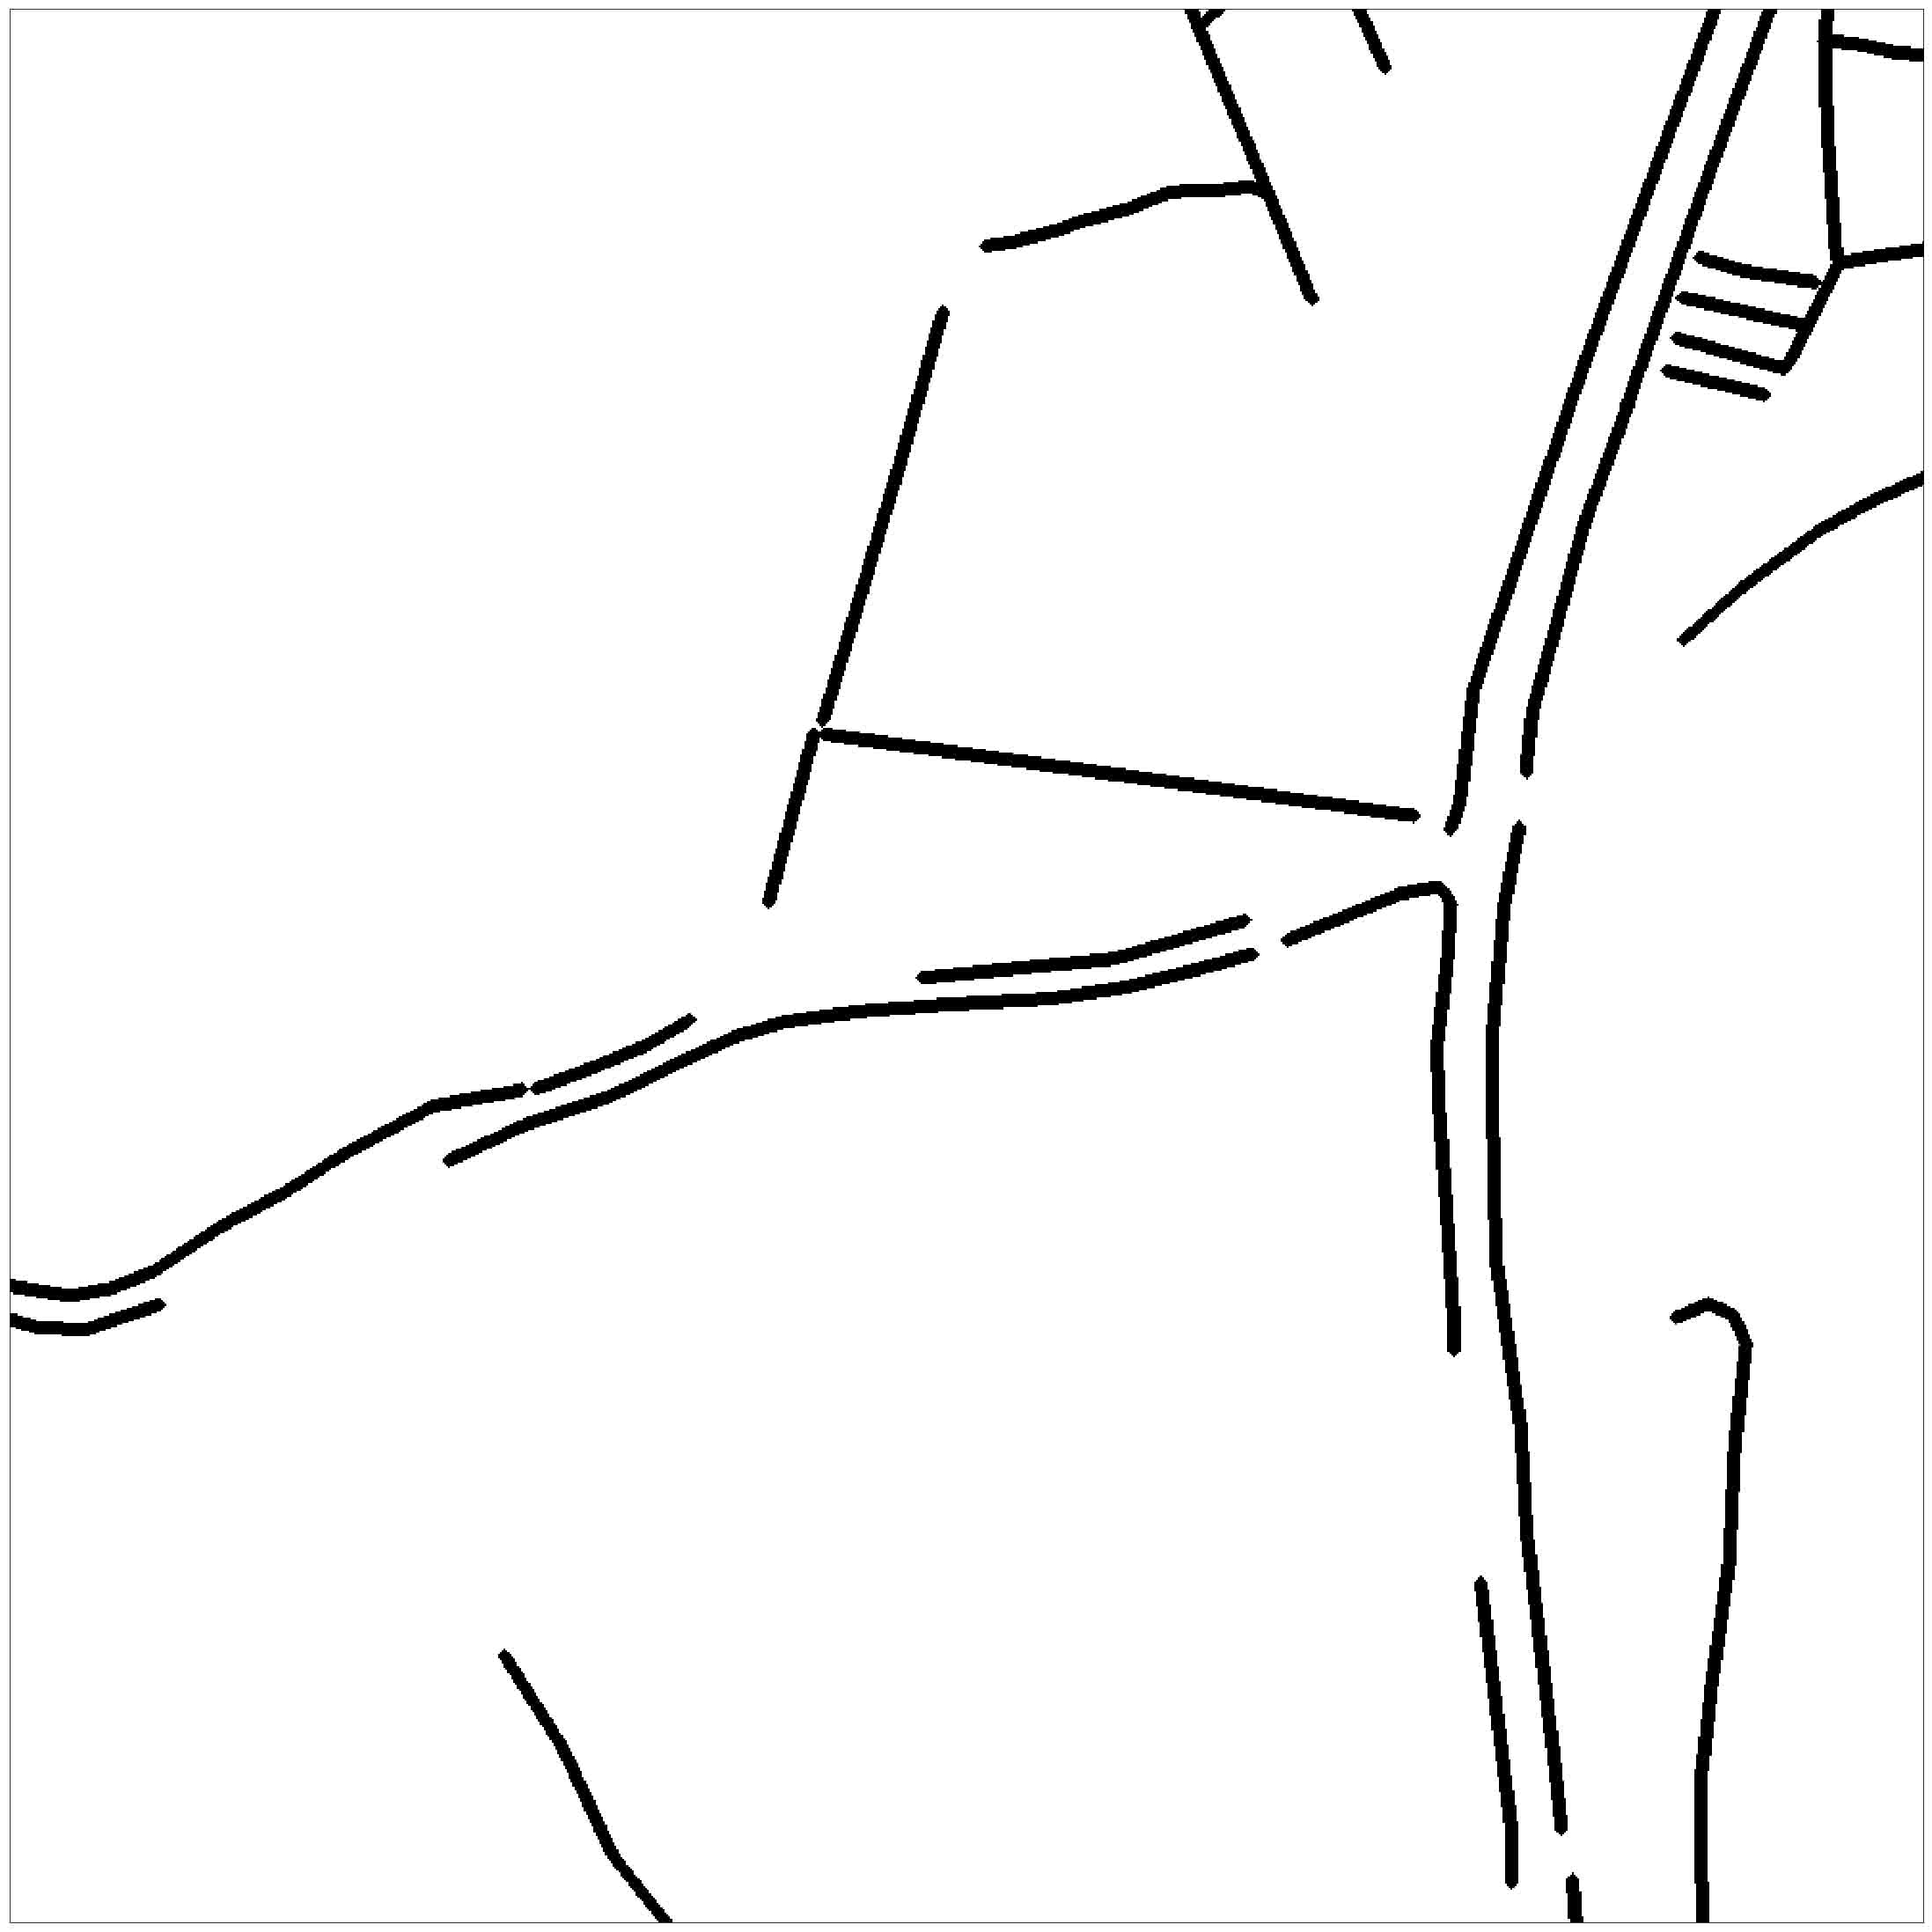
\includegraphics{./images/feature_a_lo.jpg}}}
    \subfigure[]{
        \resizebox*{3.5cm}{!}{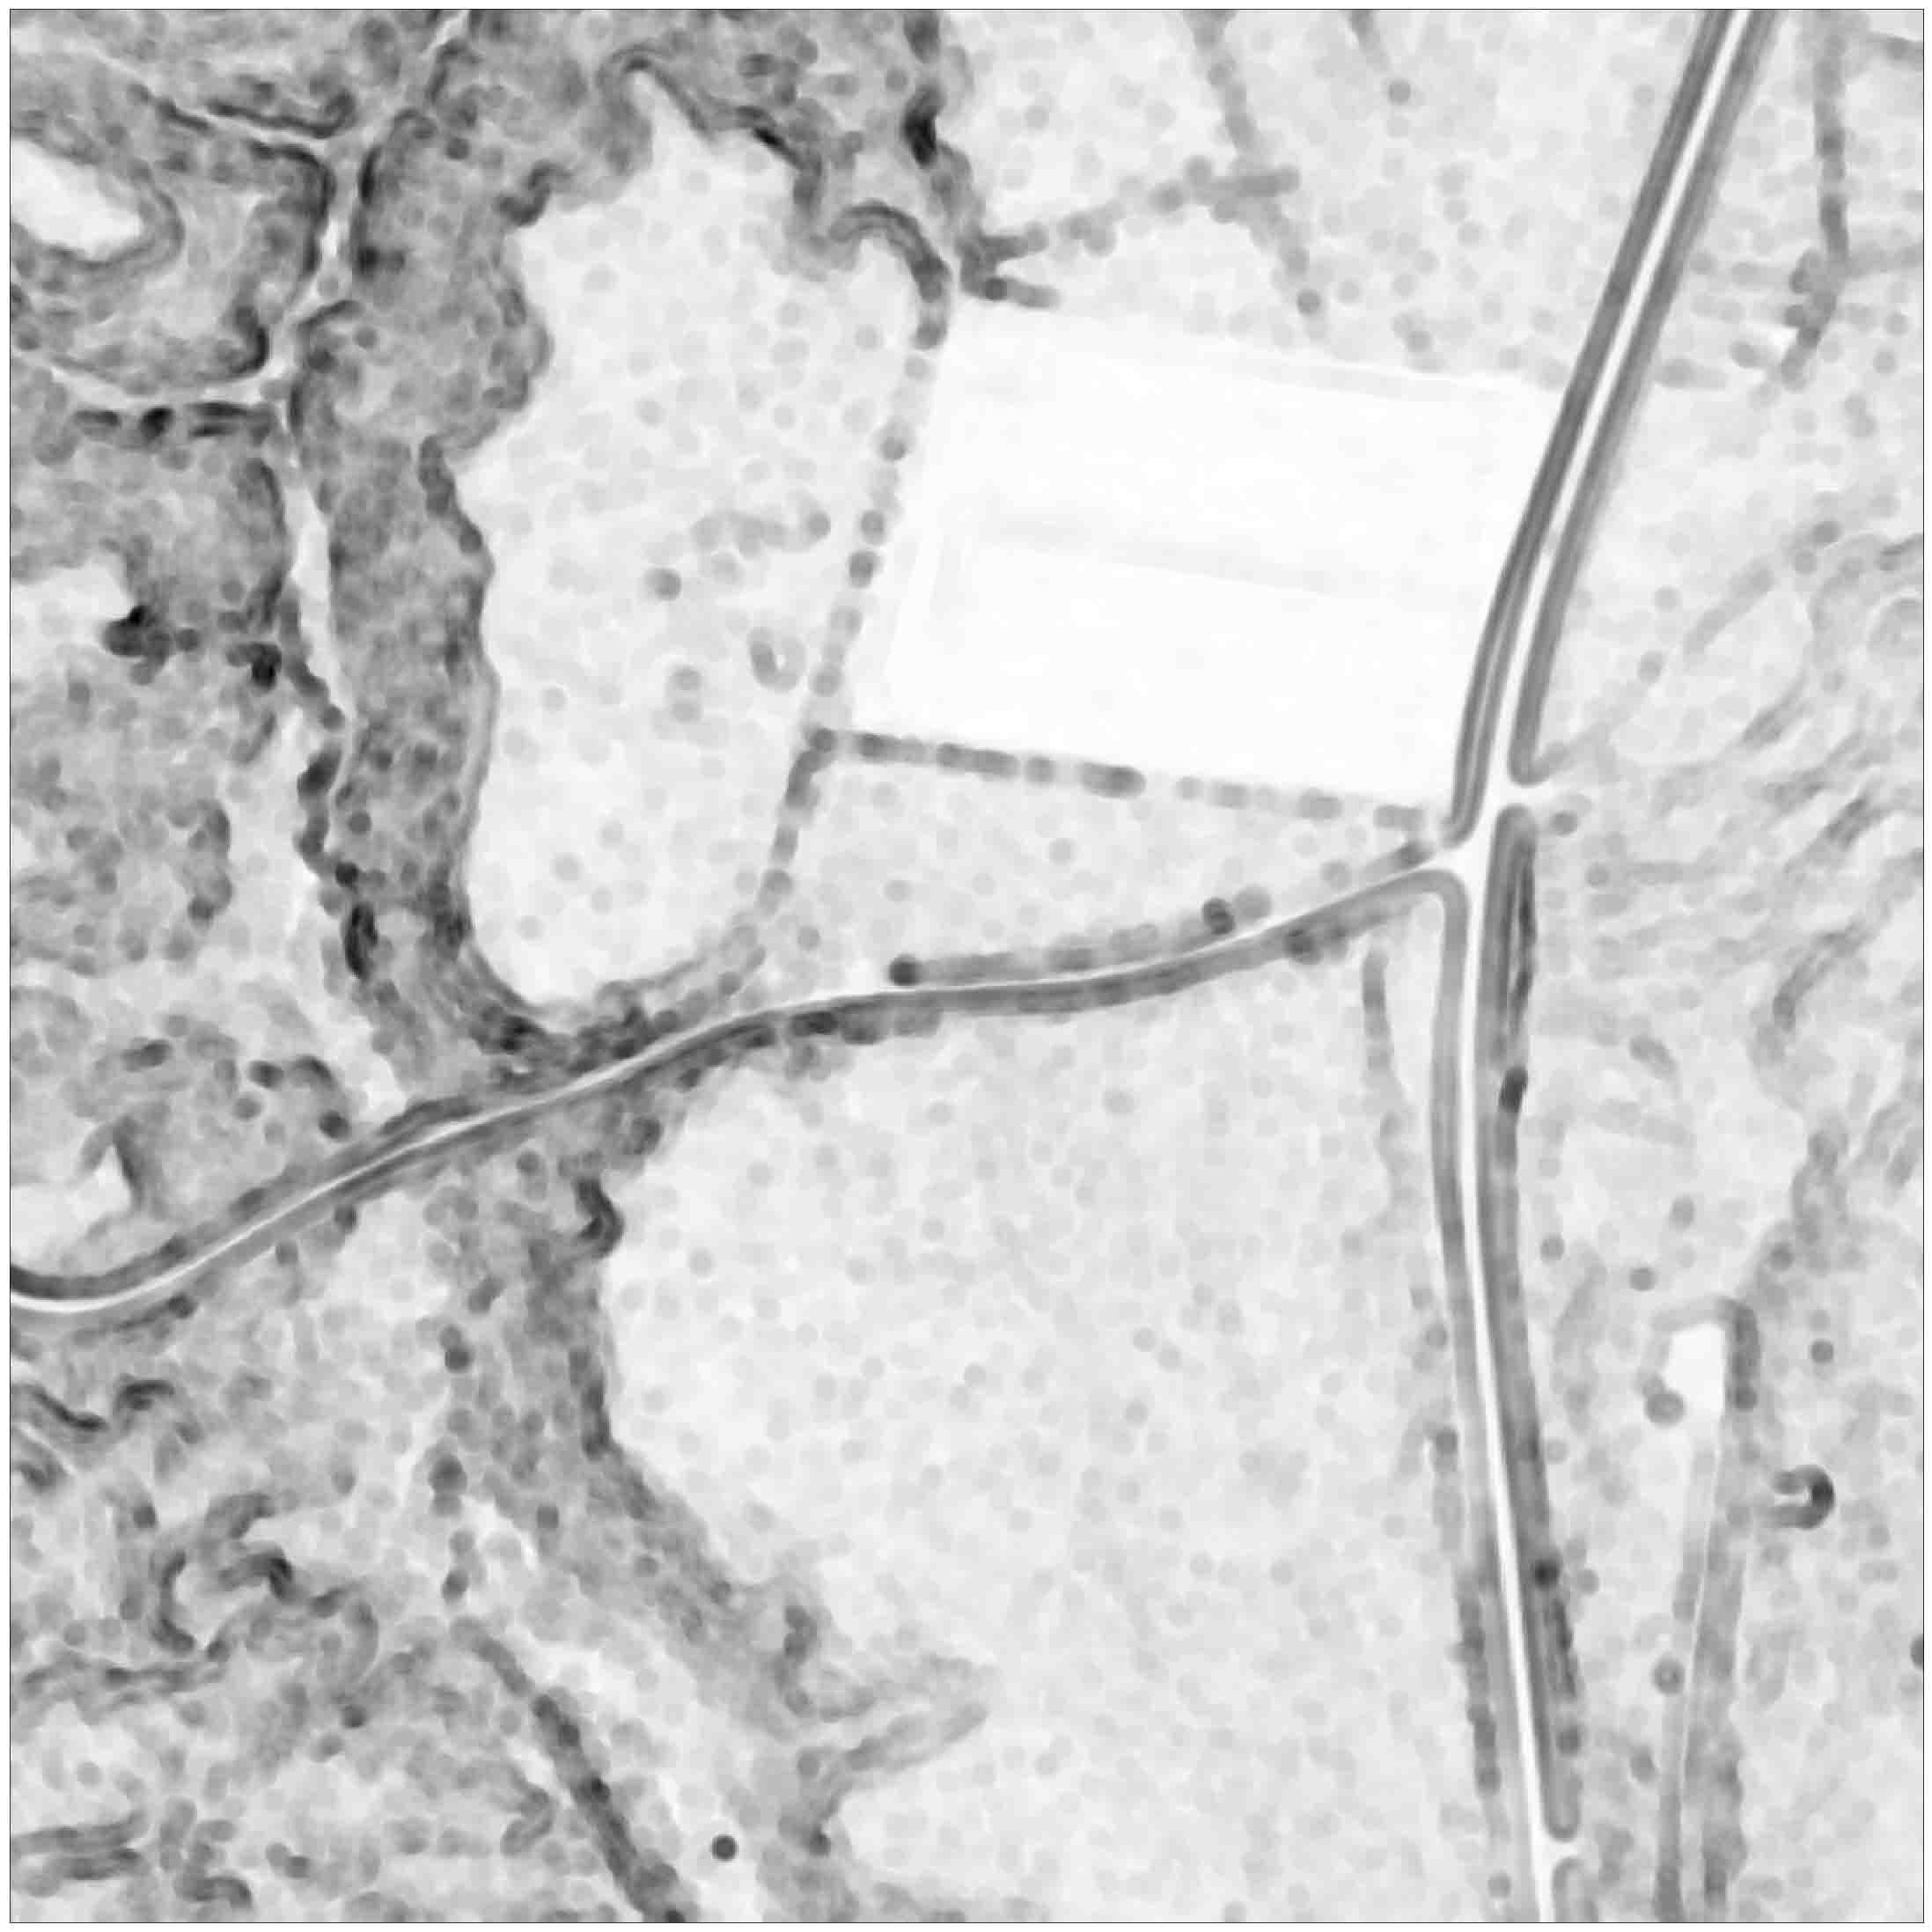
\includegraphics{./images/feature_b_lo.jpg}}}
    \subfigure[]{
        \resizebox*{3.5cm}{!}{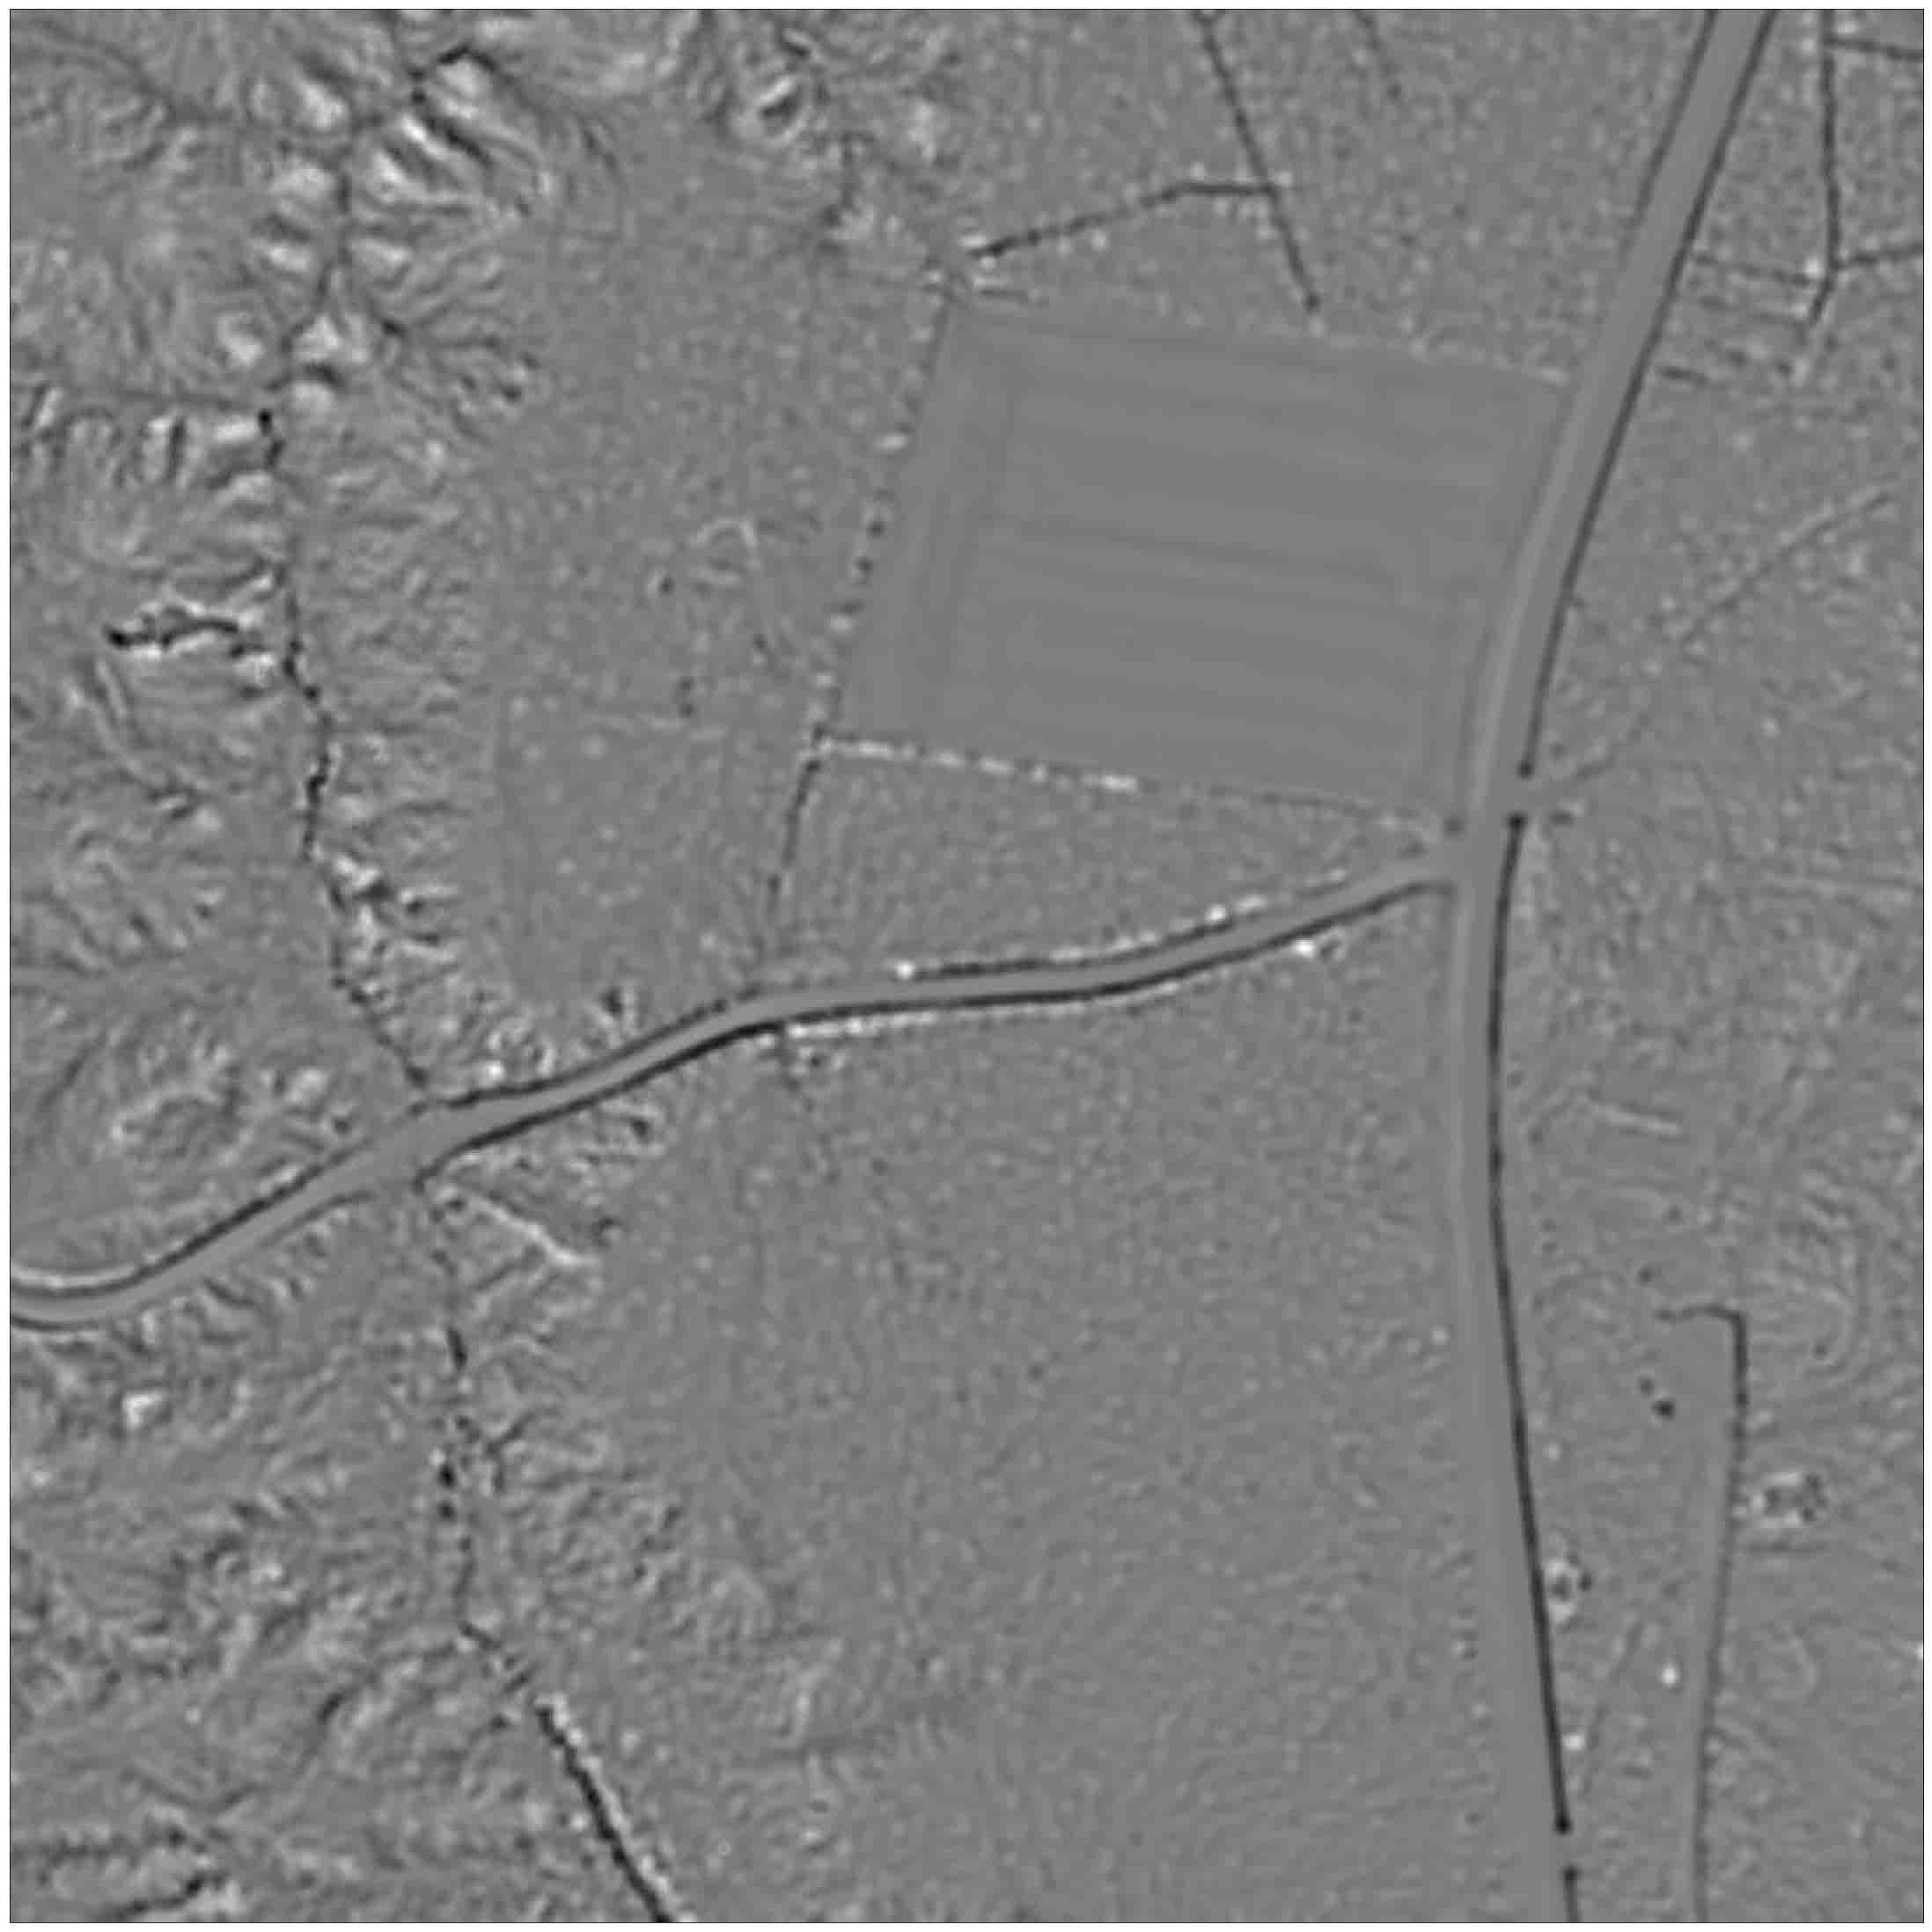
\includegraphics{./images/feature_c_lo.jpg}}}
    \subfigure[]{
        \resizebox*{3.5cm}{!}{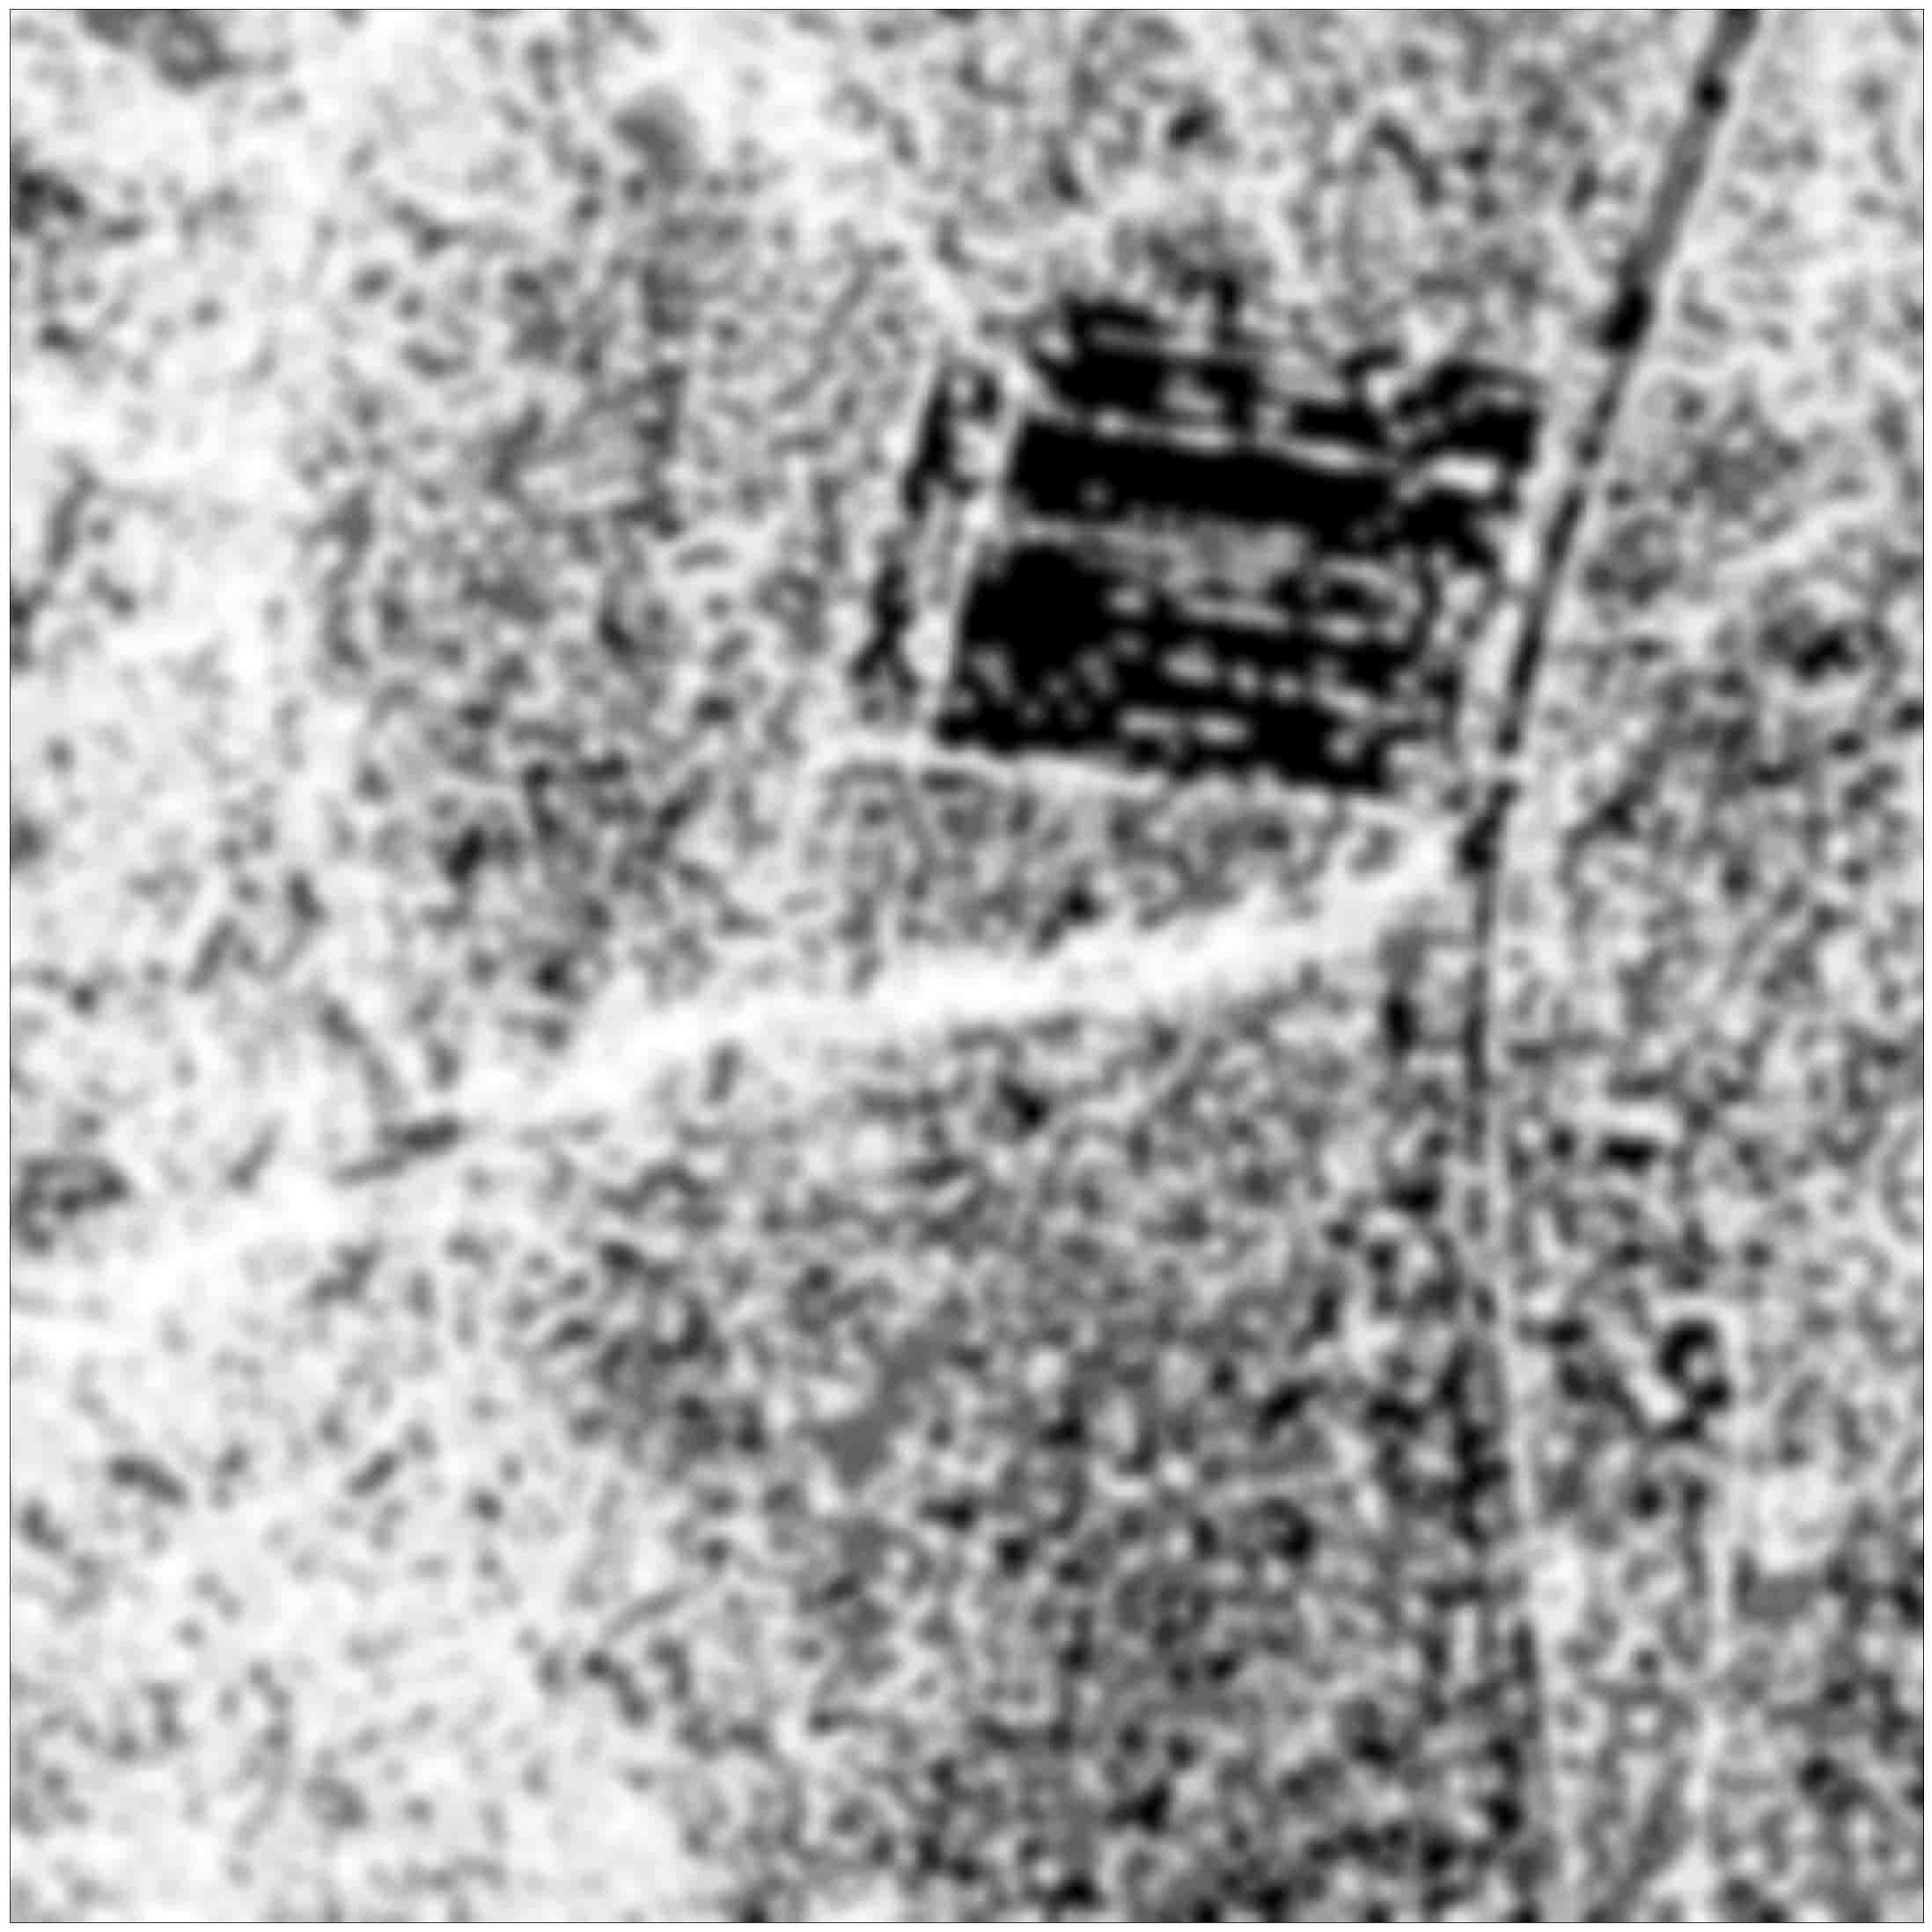
\includegraphics{./images/feature_d_lo.jpg}}}
    \subfigure[]{
        \resizebox*{3.5cm}{!}{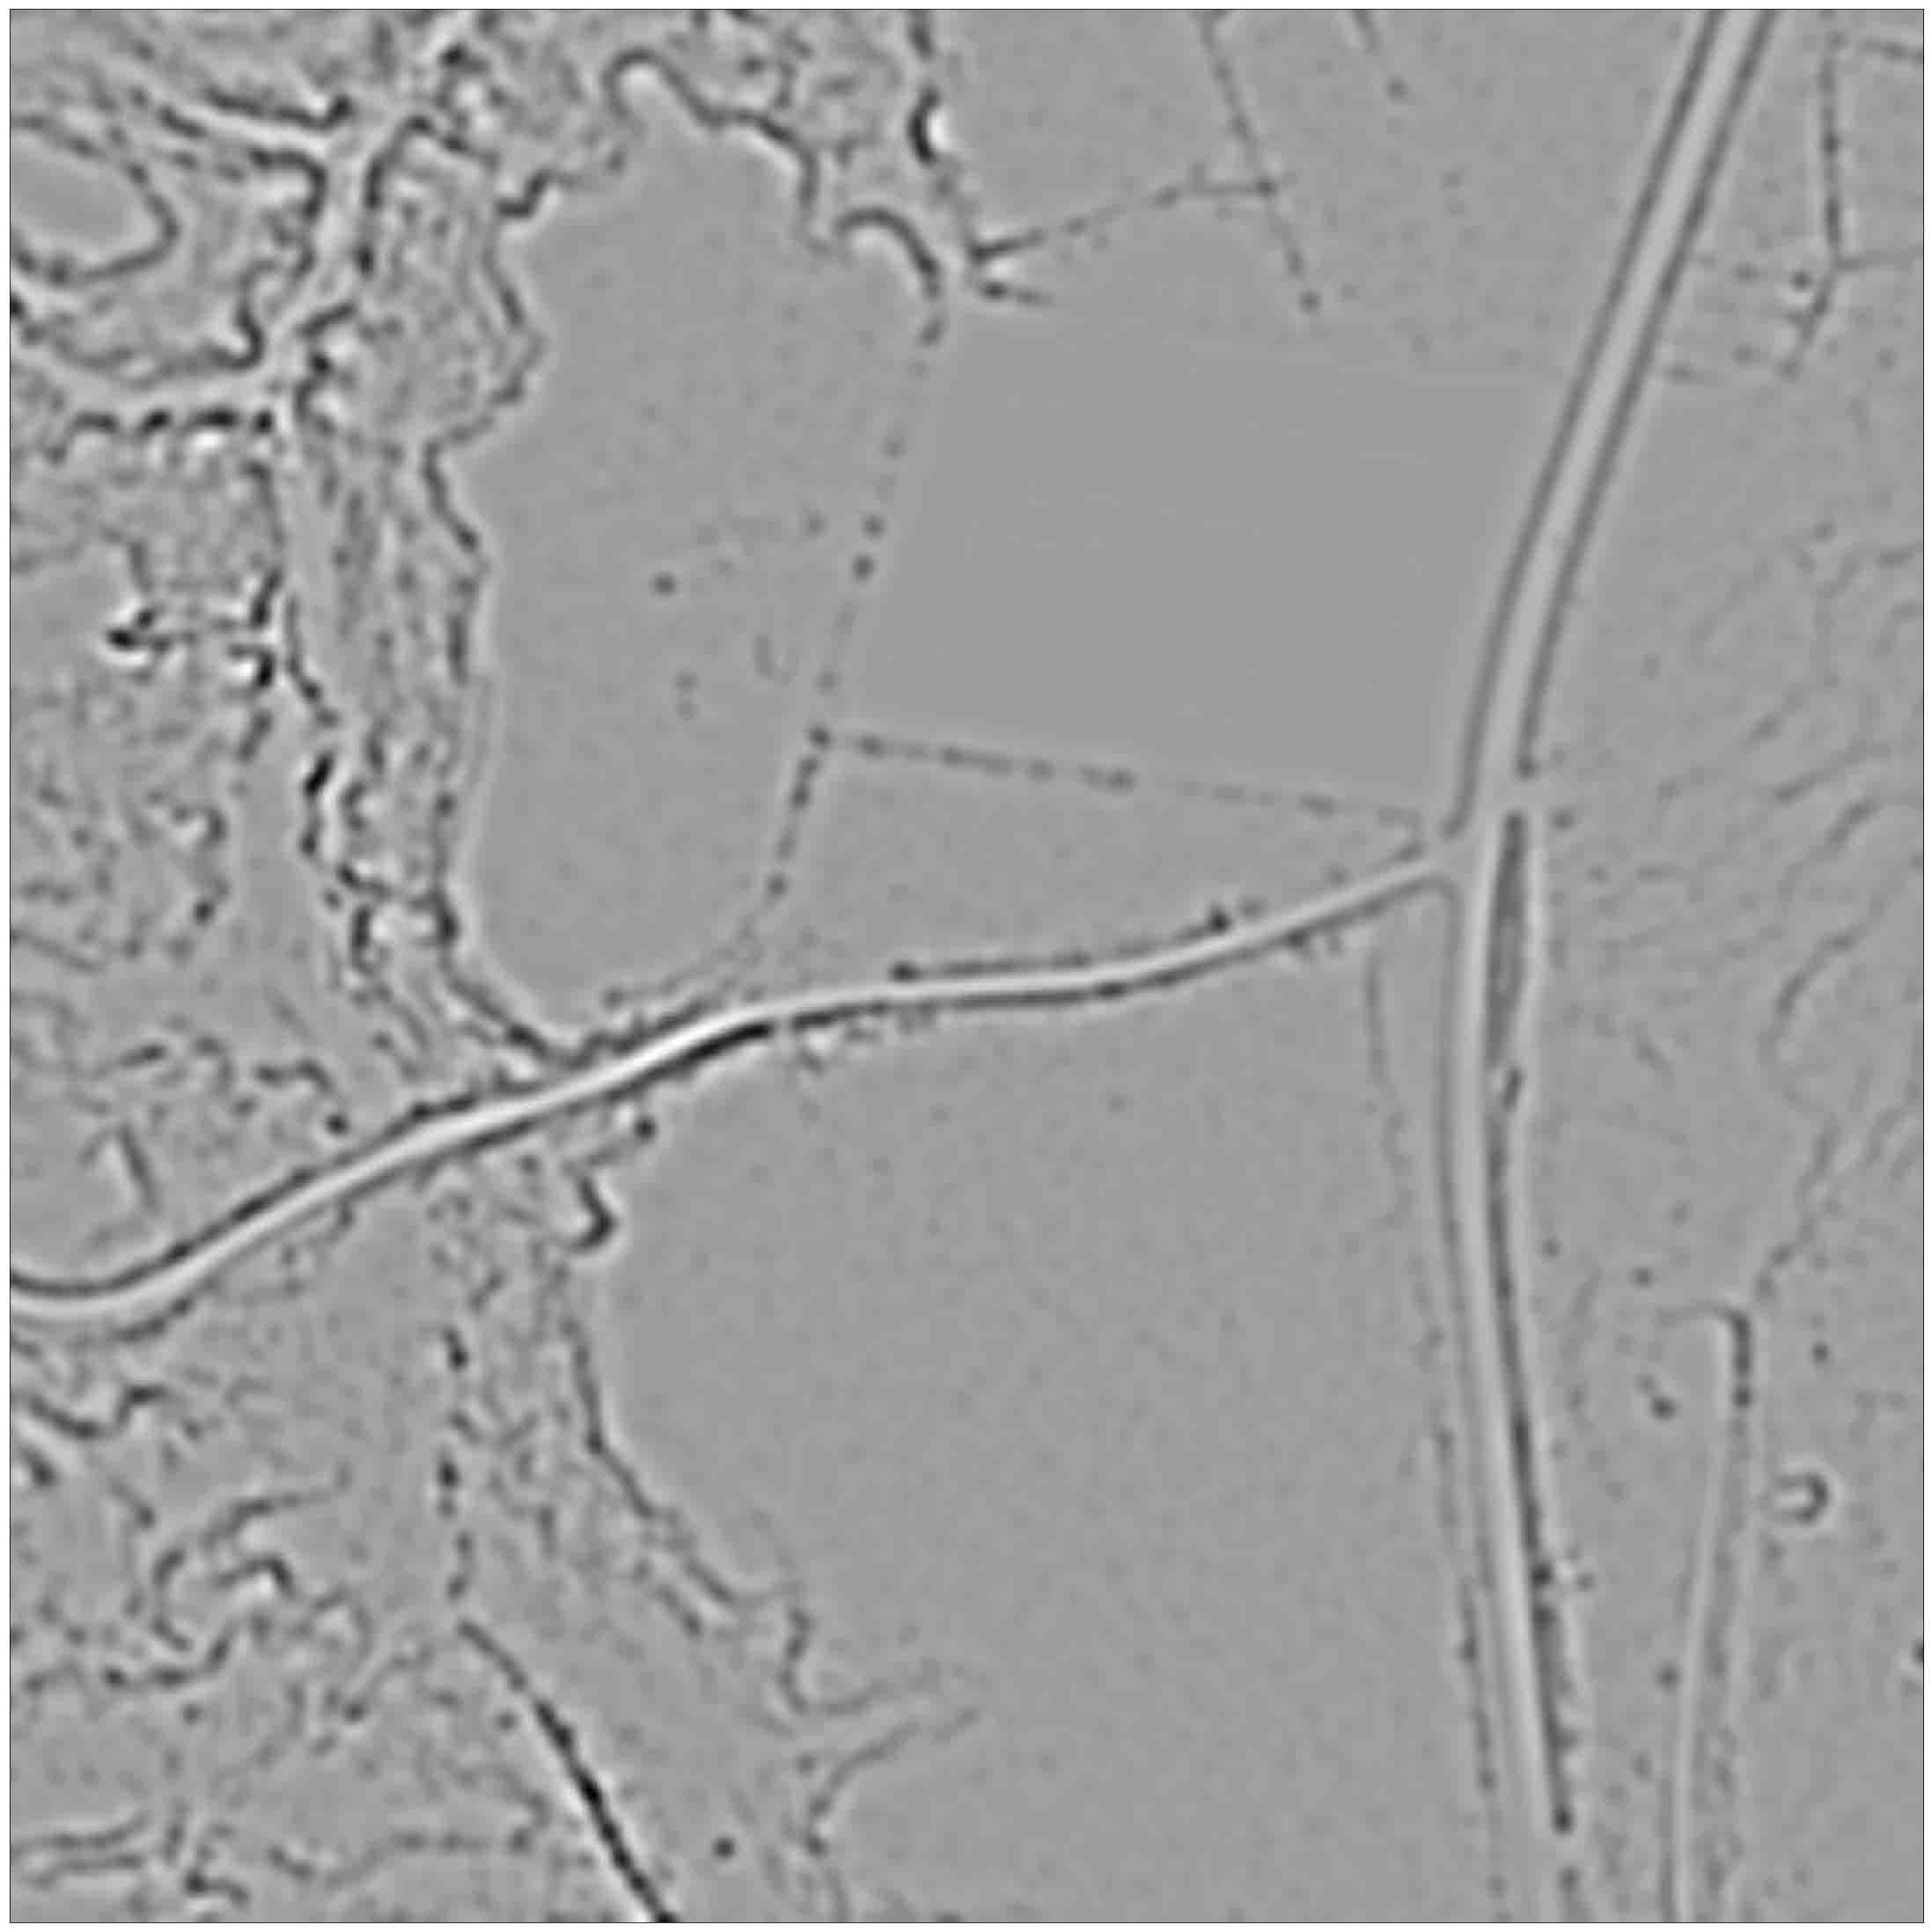
\includegraphics{./images/feature_e_lo.jpg}}}
    \subfigure[]{
        \resizebox*{3.5cm}{!}{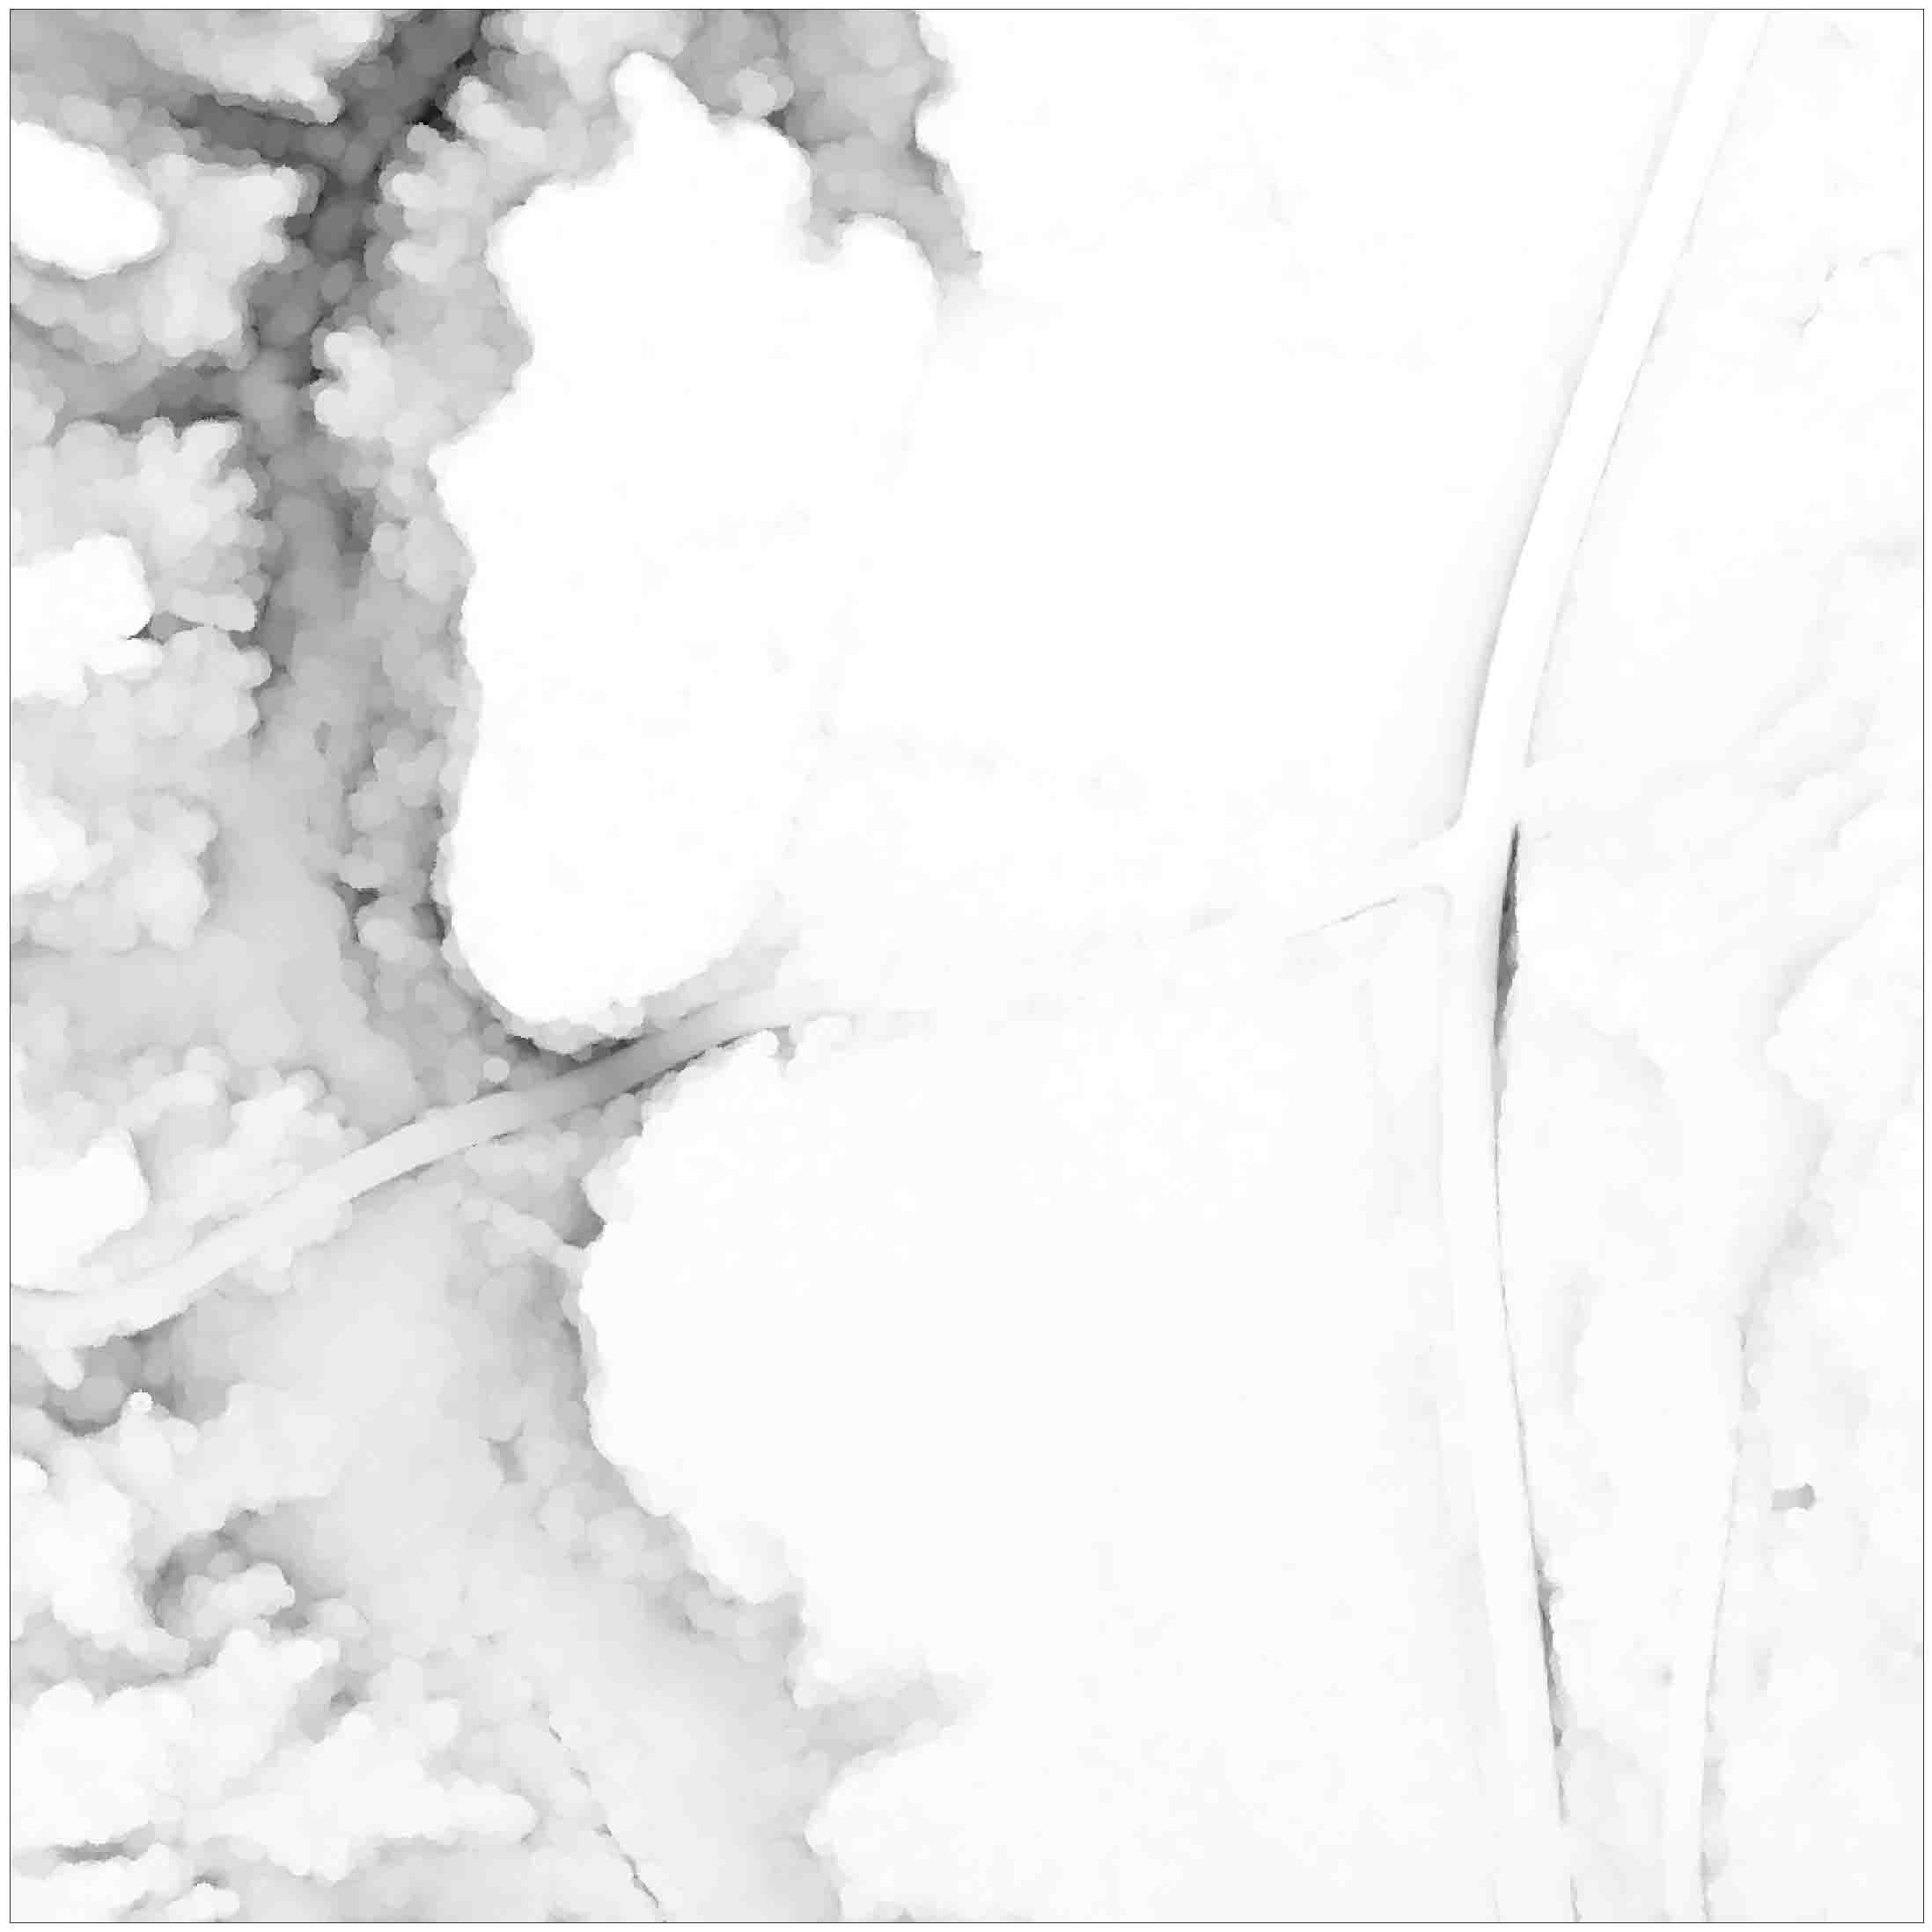
\includegraphics{./images/feature_f_lo.jpg}}}
    \subfigure[]{
        \resizebox*{3.5cm}{!}{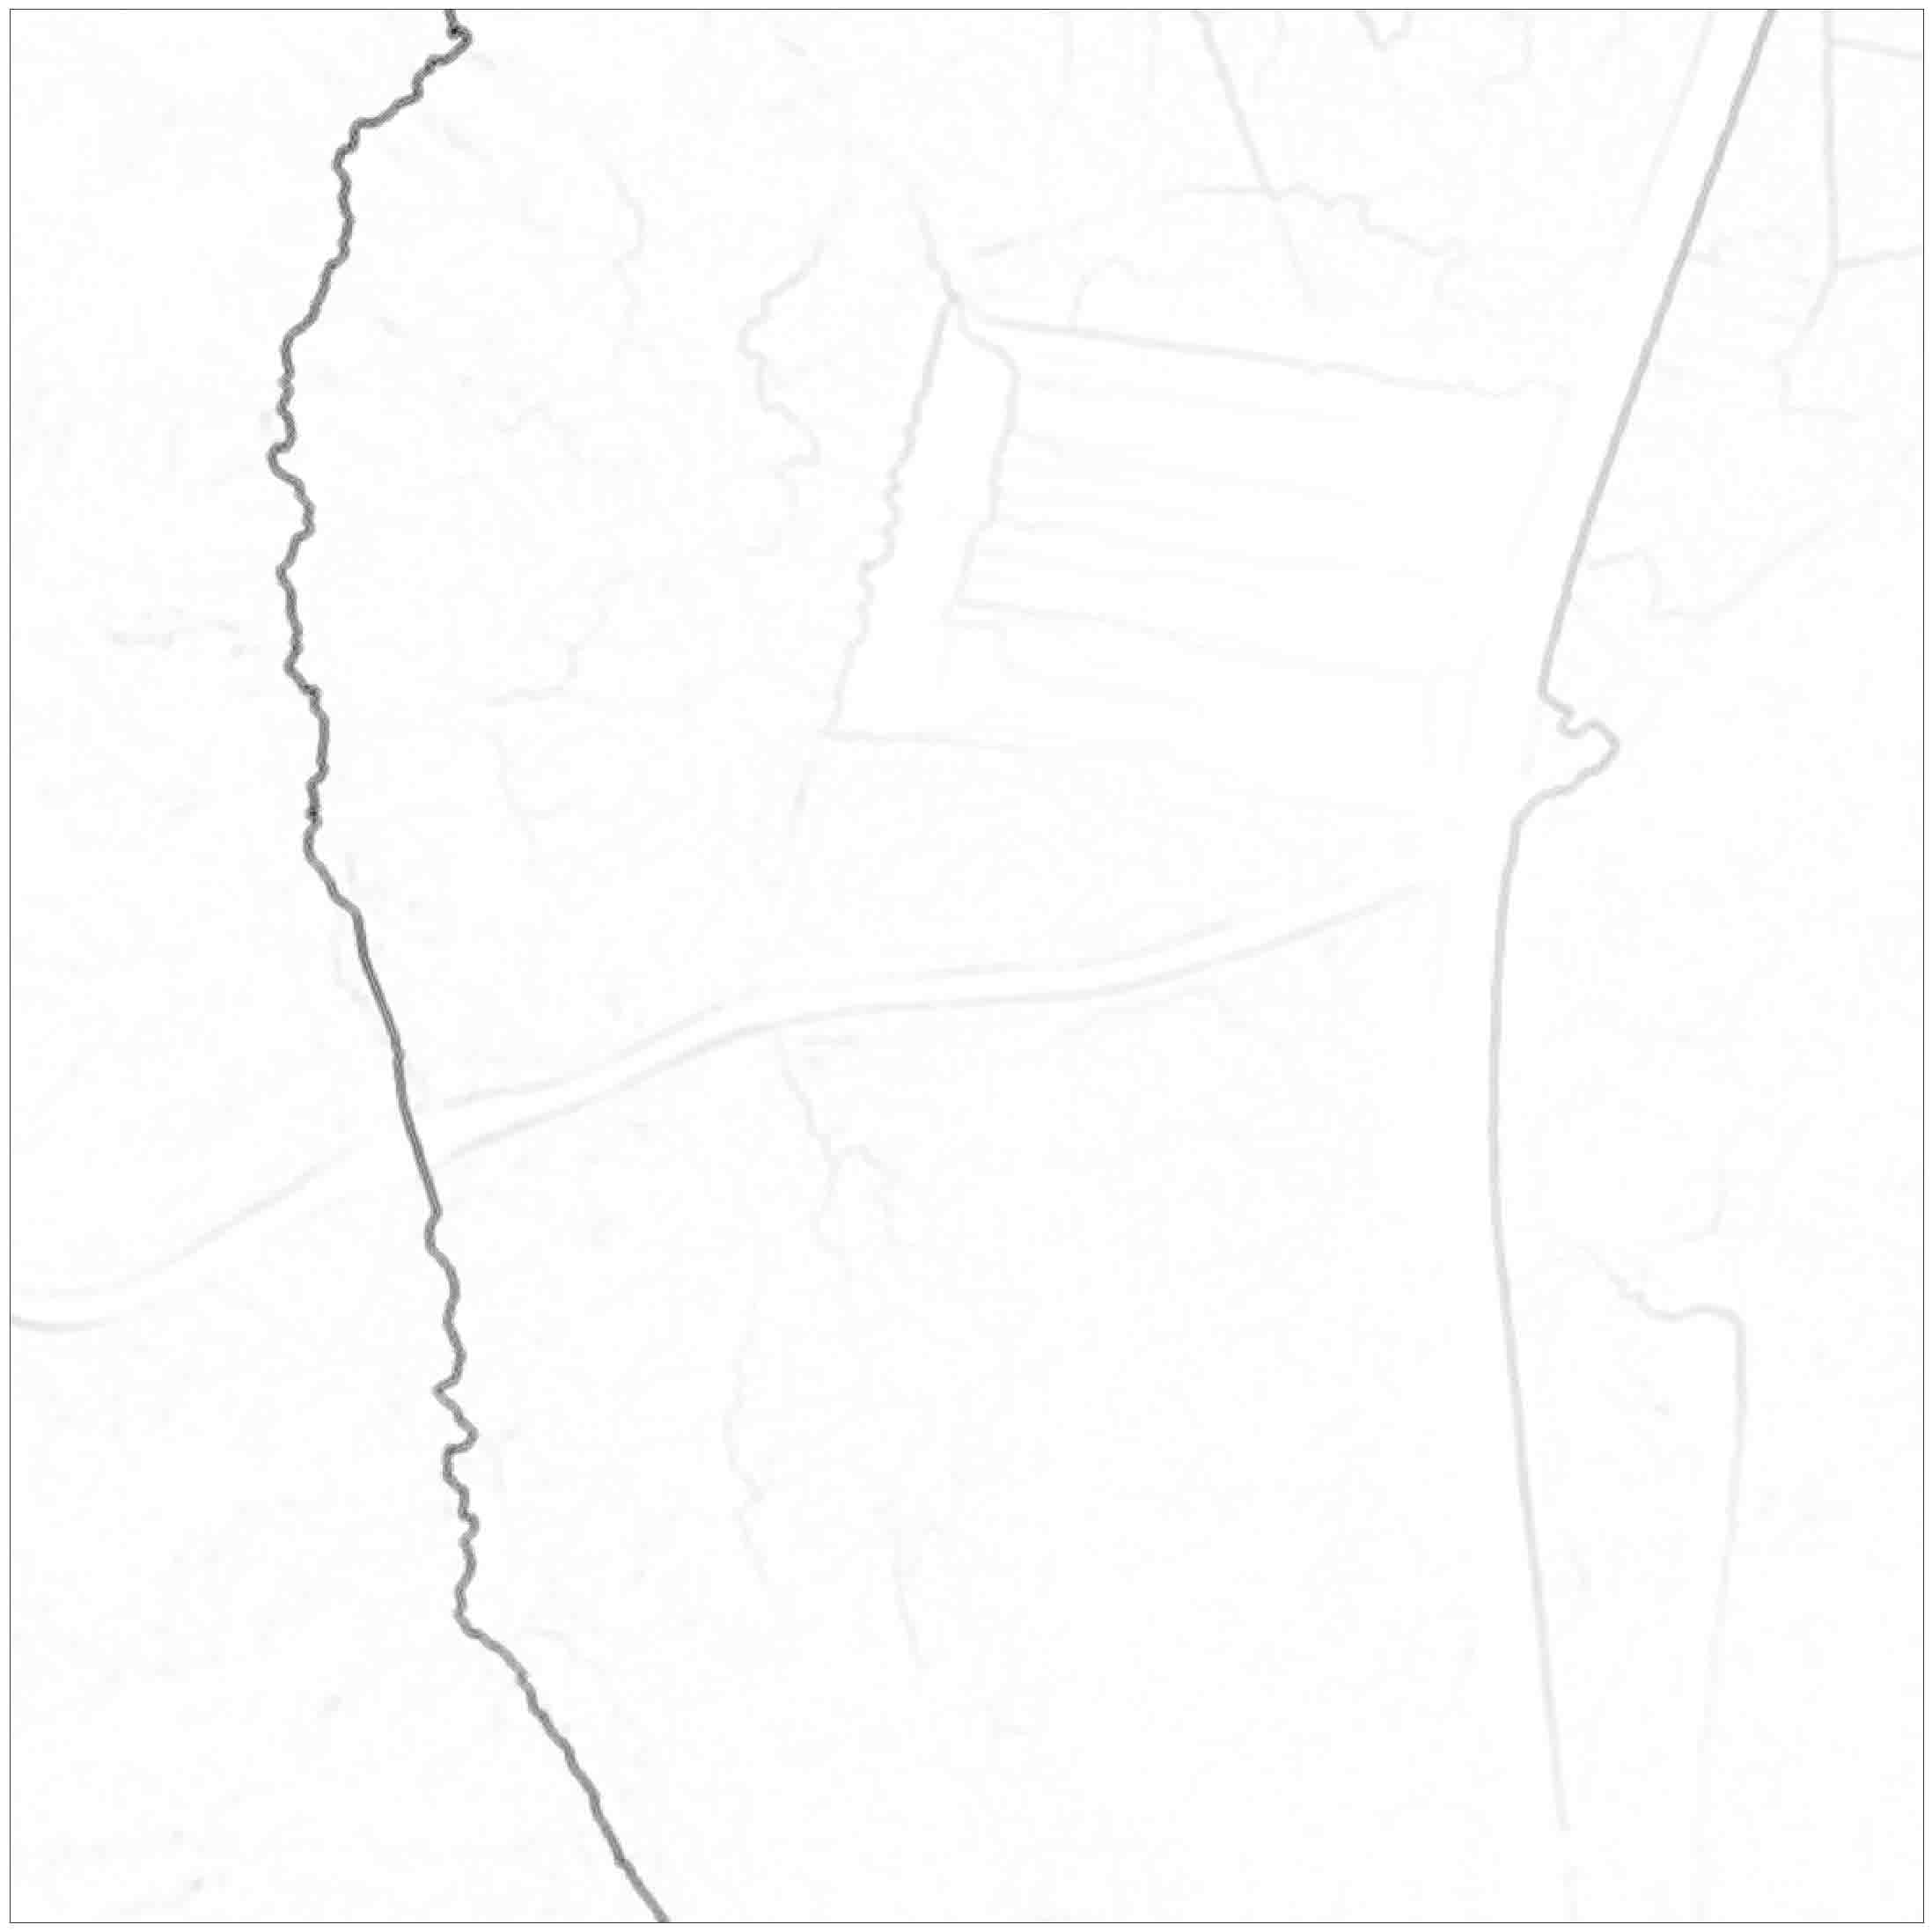
\includegraphics{./images/feature_g_lo.jpg}}}
    \subfigure[]{
        \resizebox*{3.5cm}{!}{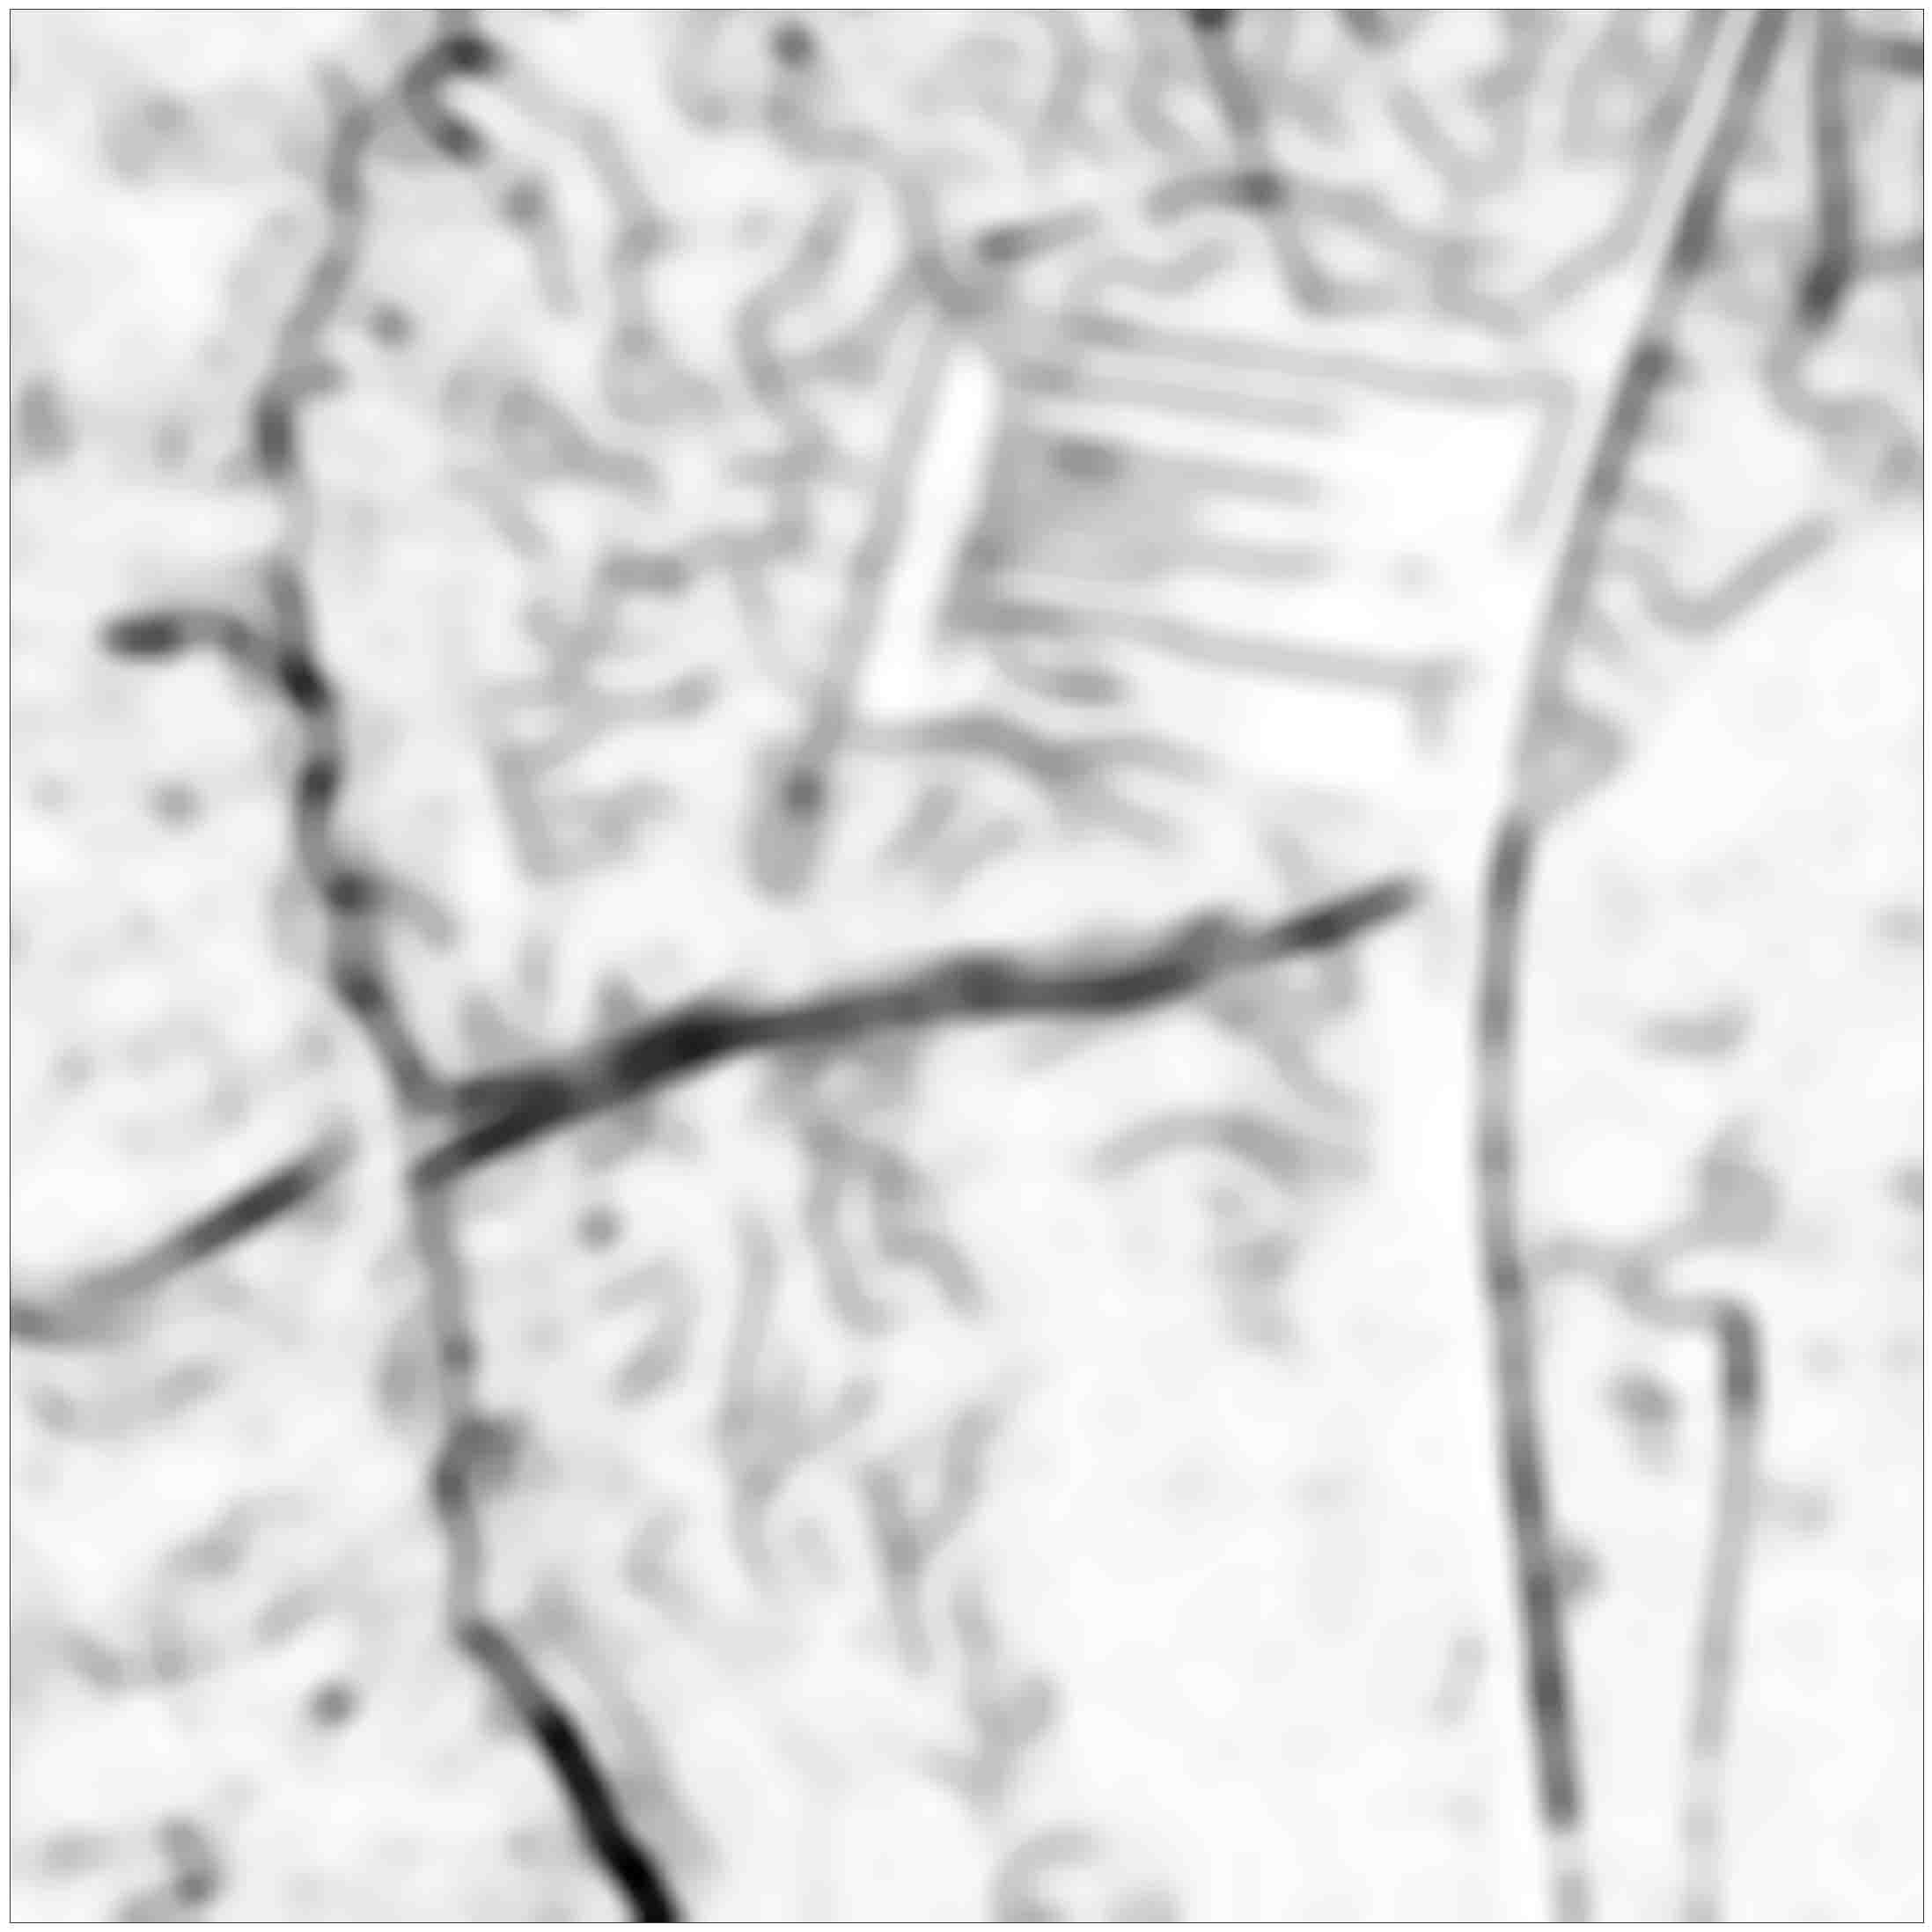
\includegraphics{./images/feature_h_lo.jpg}}}
    \subfigure[]{
        \resizebox*{3.5cm}{!}{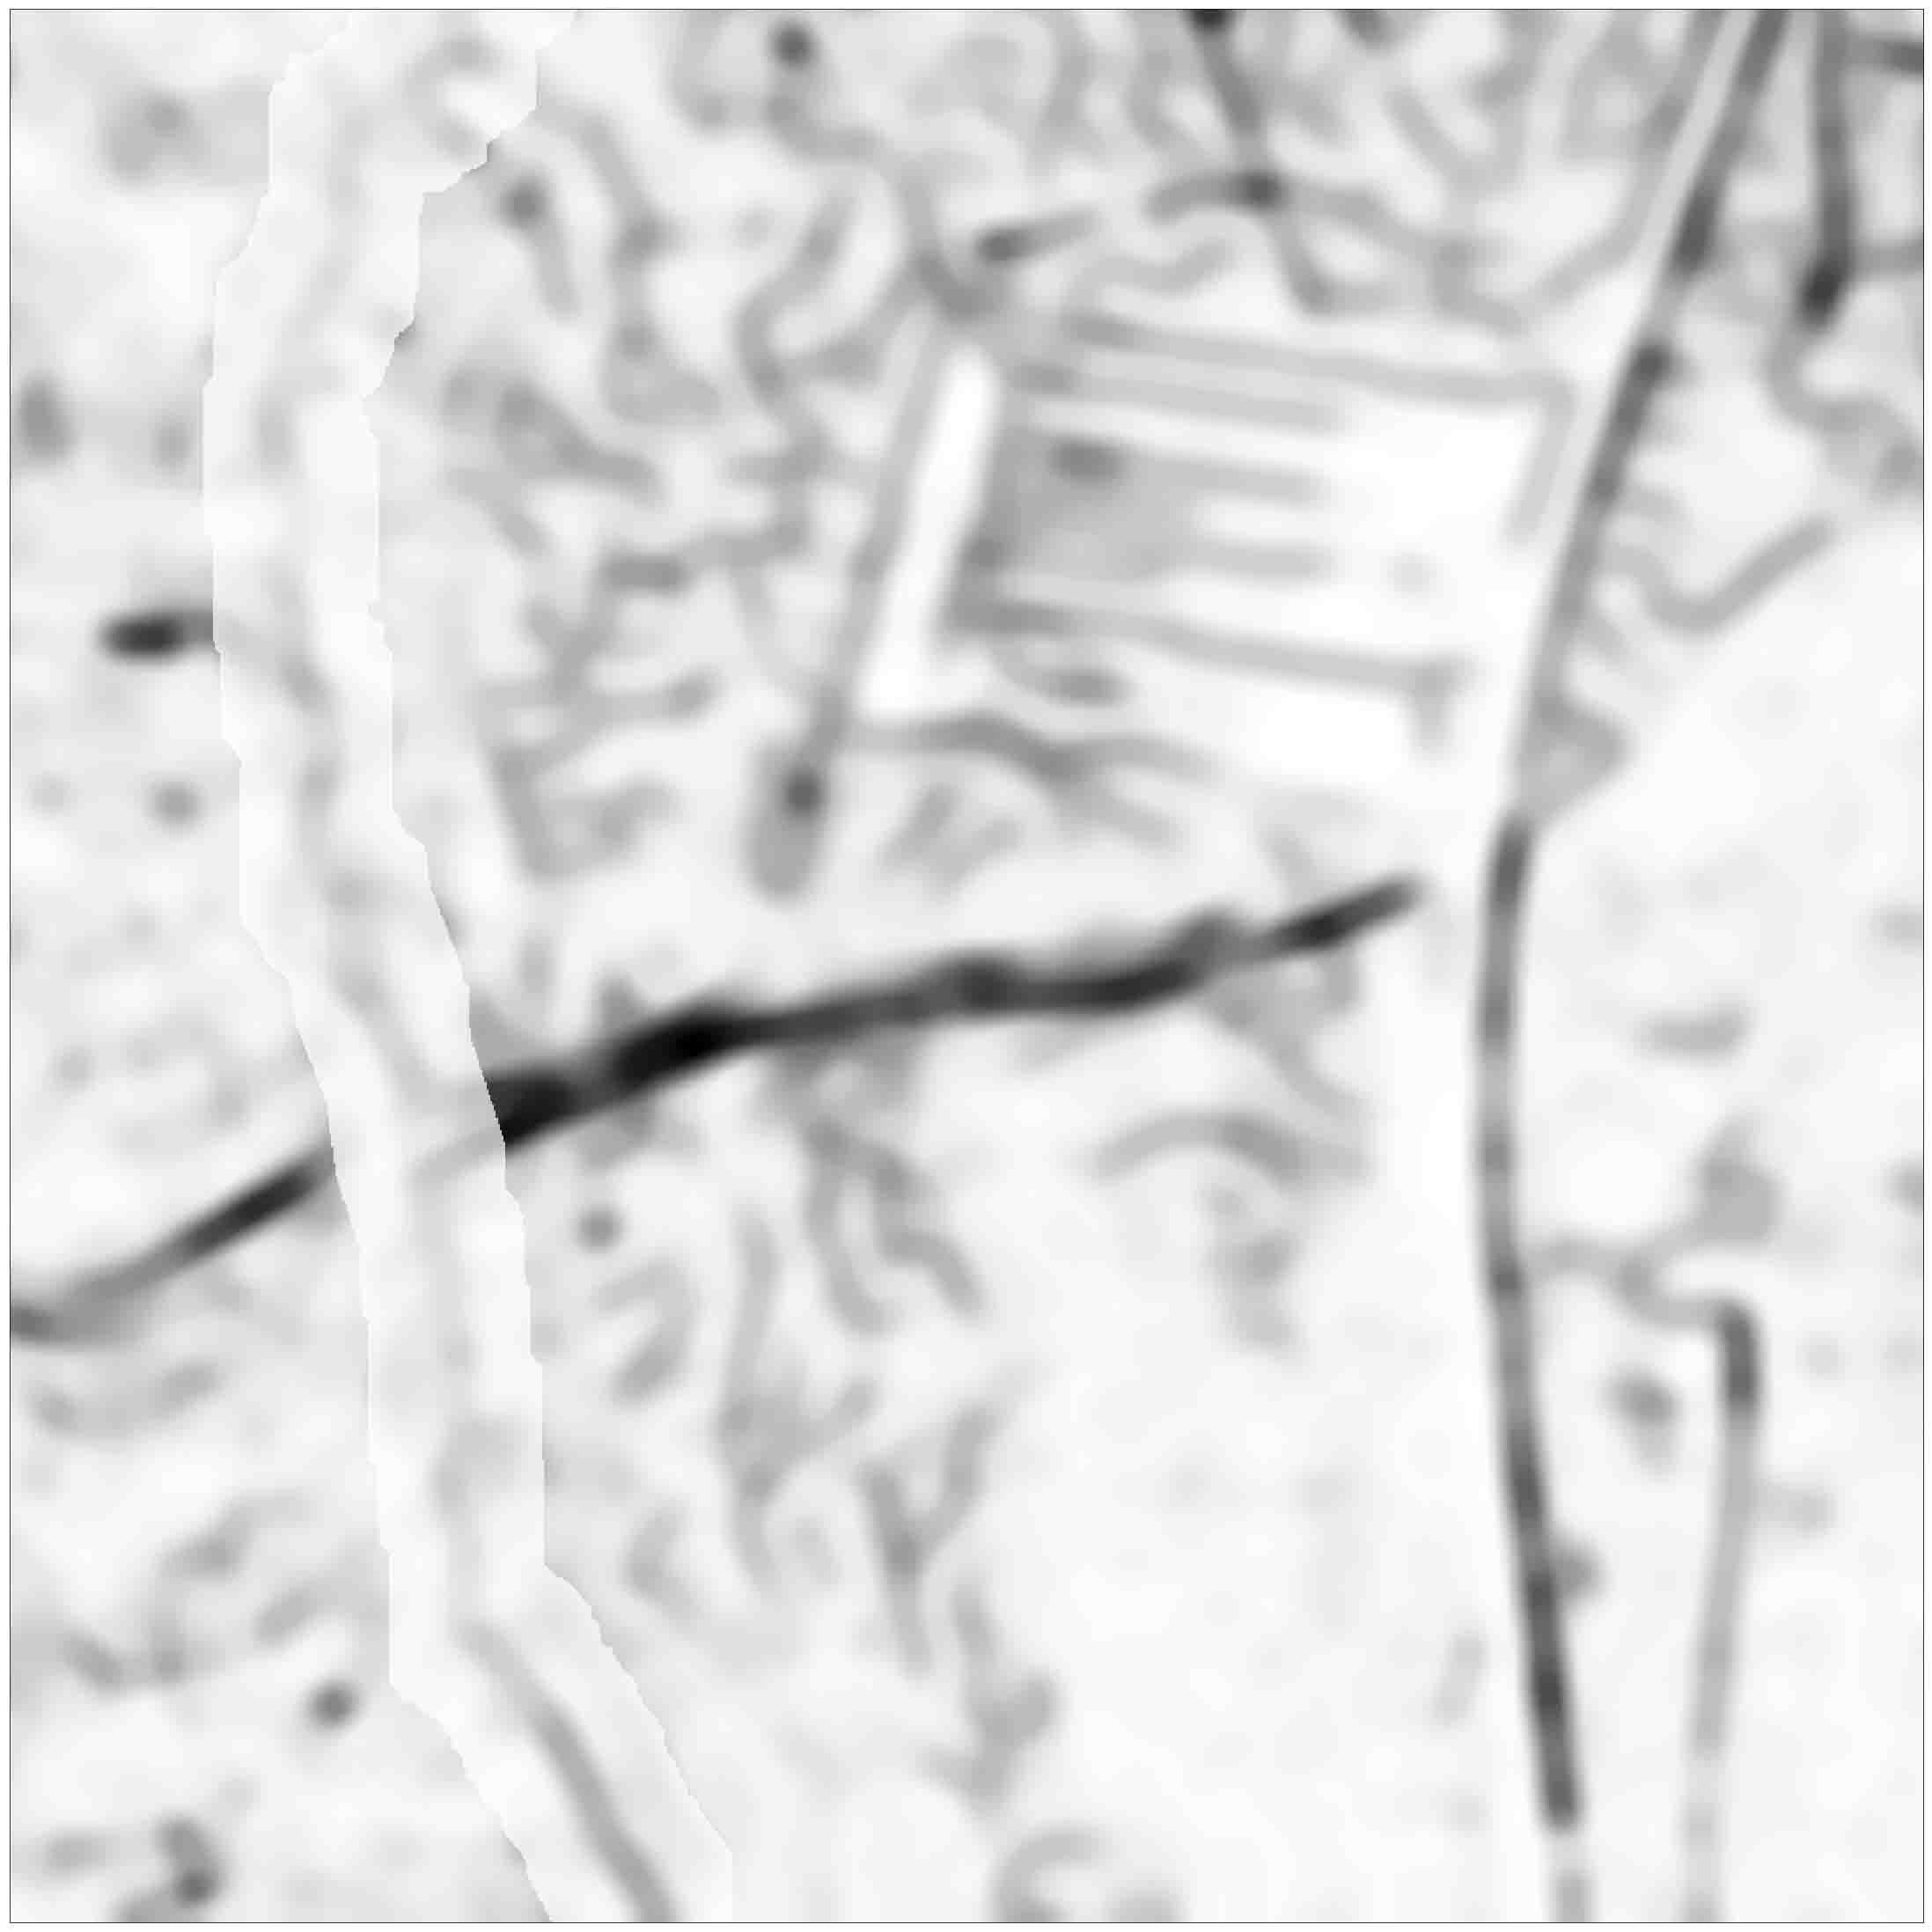
\includegraphics{./images/feature_i_lo.jpg}}}
    \caption{\textbf{Feature examples.} Shows the ditch labels as well as 8 of the 40 features for a small sample area. The radii represents pixels with a 0.5 m resolution. \newline \textbf{a:} Labelled ditches, \textbf{b:} Slope standard deviation, radius 6, \textbf{c:} HPMF mean, radius 4, \textbf{d:} HPMF ditch amplification, \textbf{e:} Sky View Factor Gabor, \textbf{f:} Sky View Factor max, radius 6, \textbf{g:} Impoundment mean, radius 3, \textbf{h:} Impoundment ditch amplification, \textbf{i:} Impoundment ditch amplification - streams removed}
    \label{fig:features}
\end{figure}

\subsubsection{Training and validation datasets}
\label{trainingvalidationdatasets}
To develop and evaluate our ditch detector, the raster and ditch label data of Krycklan were manually divided into 21 subsections, each representing an area of roughly 196 hectare (\hyperref[fig:swedenkrycklan]{Figure} \ref{fig:swedenkrycklan}). This was necessary because our method relies on the area surrounding a pixel for feature extraction, meaning it is not possible to select random pixels for training and testing. 11 of the subsections were put aside as hold-out data, only for use in the experiment to evaluate the performance of the ditch detector. The remaining 10 subsections were used solely before the experiment to develop the ditch detector, and to test different ways of preparing the data. This allowed the ditch detector to be evaluated on independent data, strengthening the validity of the experiment. \hyperref[fig:swedenkrycklan]{Figure} \ref{fig:swedenkrycklan} shows which subsections were used for development and evaluation respectively. The 11 hold-out subsections were used as folds in an 11-fold cross validation in the final experiment.

\subsection{Developing the Random Forests model}

The Random Forests \citep{breiman} algorithm from the Python library \textit{scikit-learn} \citep{scikit-learn} was used in the experiment, and the classifiers were trained on the 40 features seen in \hyperref[featuretable]{Table} \ref{featuretable}. A byproduct of the training is the Gini importance, which denotes the most important features \citep{gini}. For our study, a hyperparameter tuning showed that using 300 trees and \textit{gini} as the splitting criterion, with a minimum of 10 samples per node split, and no artificial class weight or max depth of trees yielded the best predictions. The testing phase showed that, due to the class imbalance (only 2\% of pixels being ditch pixels), the model was not being punished for mislabelling ditches as non-ditches. To combat this, we evened out the amount of ditch and non-ditch instances in the training data by first extracting all pixels labelled as ditches as well as pixels within close proximity of ditches. Second, pixels were sampled randomly from the entire subsection to still capture most of the geographical features of each area (\hyperref[fig:balancedmasks]{Figure} \ref{fig:balancedmasks}).

\begin{table} [!htb]
\centering
    {\begin{tabular}{ll}
      \textbf{Terrain Index/Algorithm}\textsuperscript{a} & \textbf{Circular radii}\textsuperscript{b} \\ 
      \hline
      Sky View Factor median &2, 6 \\
      Sky View Factor standard deviation & 6 \\
      Sky View Factor min & 6 \\
      Sky View Factor max & 2, 4, 6 \\
      Sky View Factor non ditch amplification & - \\ 
      Sky View Factor Gabor & - \\
      Sky View Factor Gabor - streams removed & -\\
      
      Impoundment mean & 2, 3, 4, 6 \\
      Impoundment median & 2, 4, 6 \\
      Impoundment standard deviation & 4, 6 \\
      Impoundment max & 6 \\
      Impoundment ditch amplification & - \\
      Impoundment ditch amplification - streams removed & - \\
      
      HPMF mean & 3, 4, 6 \\
      HPMF median & 4 \\
      HPMF standard deviation & 6 \\
      HPMF min & 2, 4 \\
      HPMF ditch amplification & - \\
      HPMF ditch amplification - streams removed & - \\
      HPMF Gabor - streams removed & -\\
      
      Slope mean & 6 \\
      Slope median & 6 \\
      Slope standard deviation & 4, 6 \\
      Slope min & 2, 4, 6 \\
      Slope non-ditch amplification & - \\
      \hline
    \end{tabular}}
    \caption{\textbf{Feature set.} The 40 features used to train the models.
    \newline \textsuperscript{a} The algorithm used to produce the feature. \newline
        \textsuperscript{b} Represents the radius of the circular mask (if one was used) to determine which neighbouring pixels to use in the aggregation. The radii represents pixels with a 0.5 m resolution.}
    \label{featuretable}
\end{table}

\begin{figure} [!htb]
    \centering
    \subfigure[]{
        \resizebox*{5.6cm}{!}{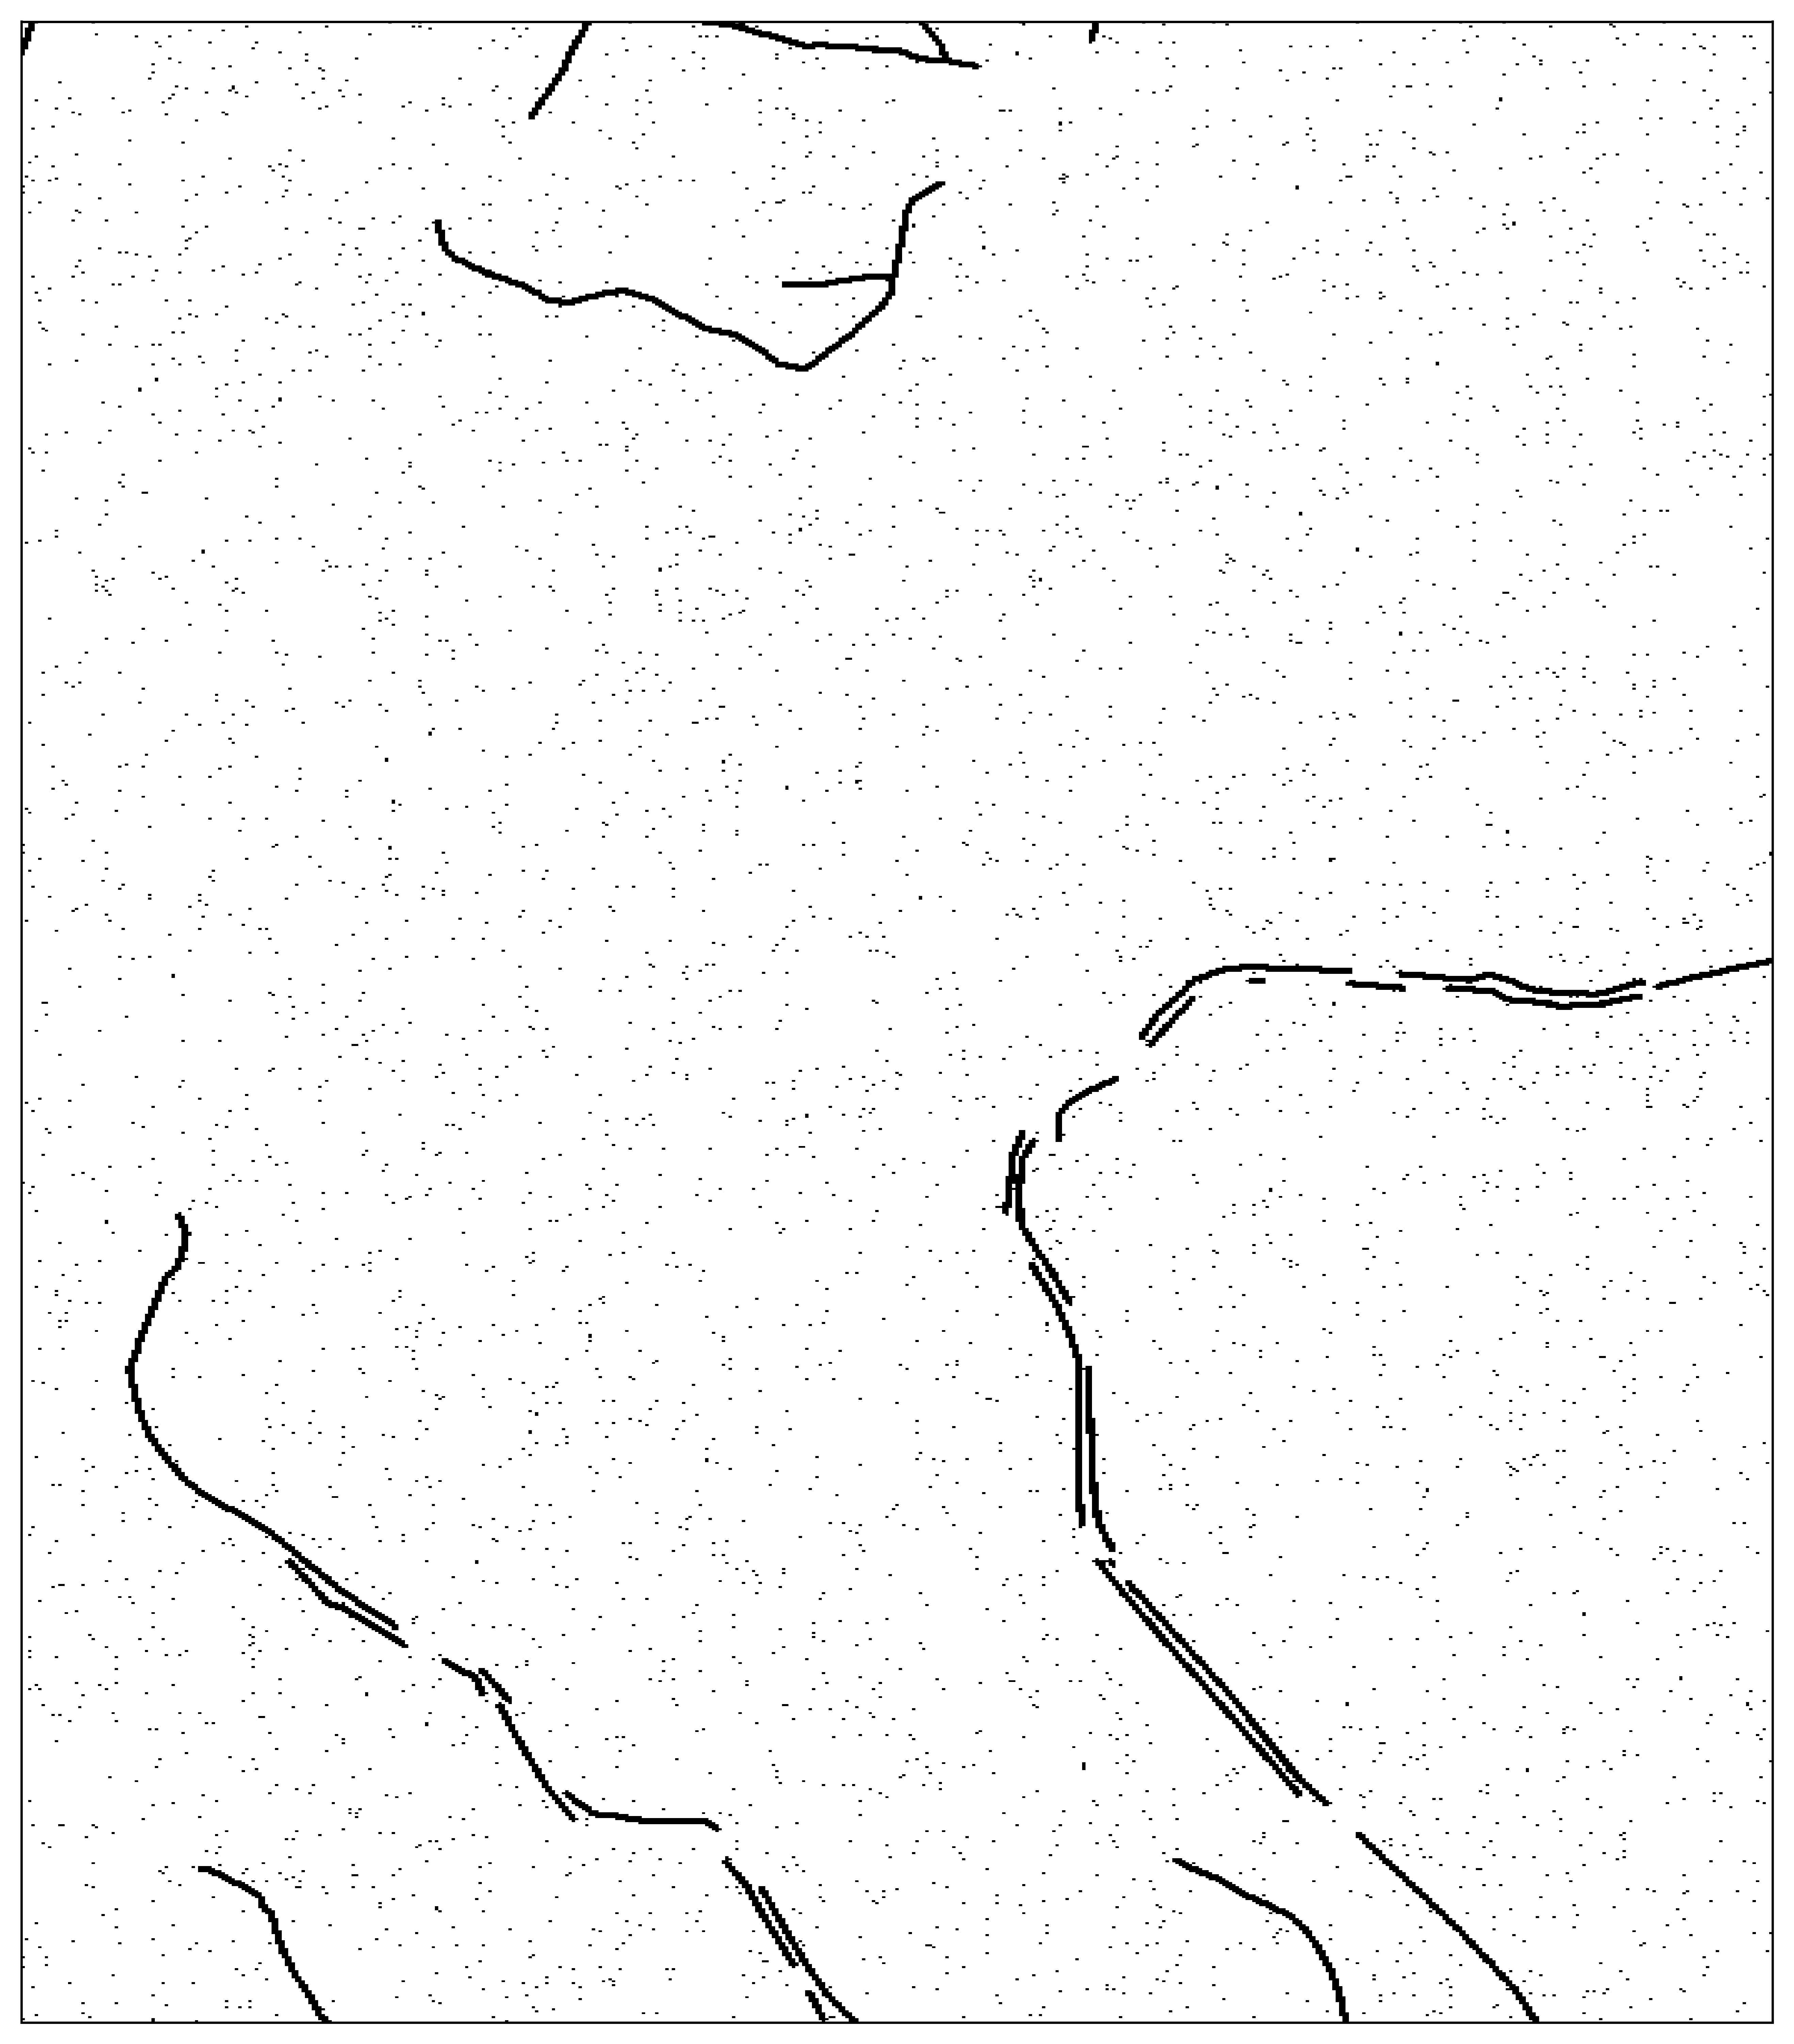
\includegraphics{./images/publ_balanced_masks_A_lo.jpg}}}\hspace{5pt}
    \subfigure[]{
        \resizebox*{5.6cm}{!}{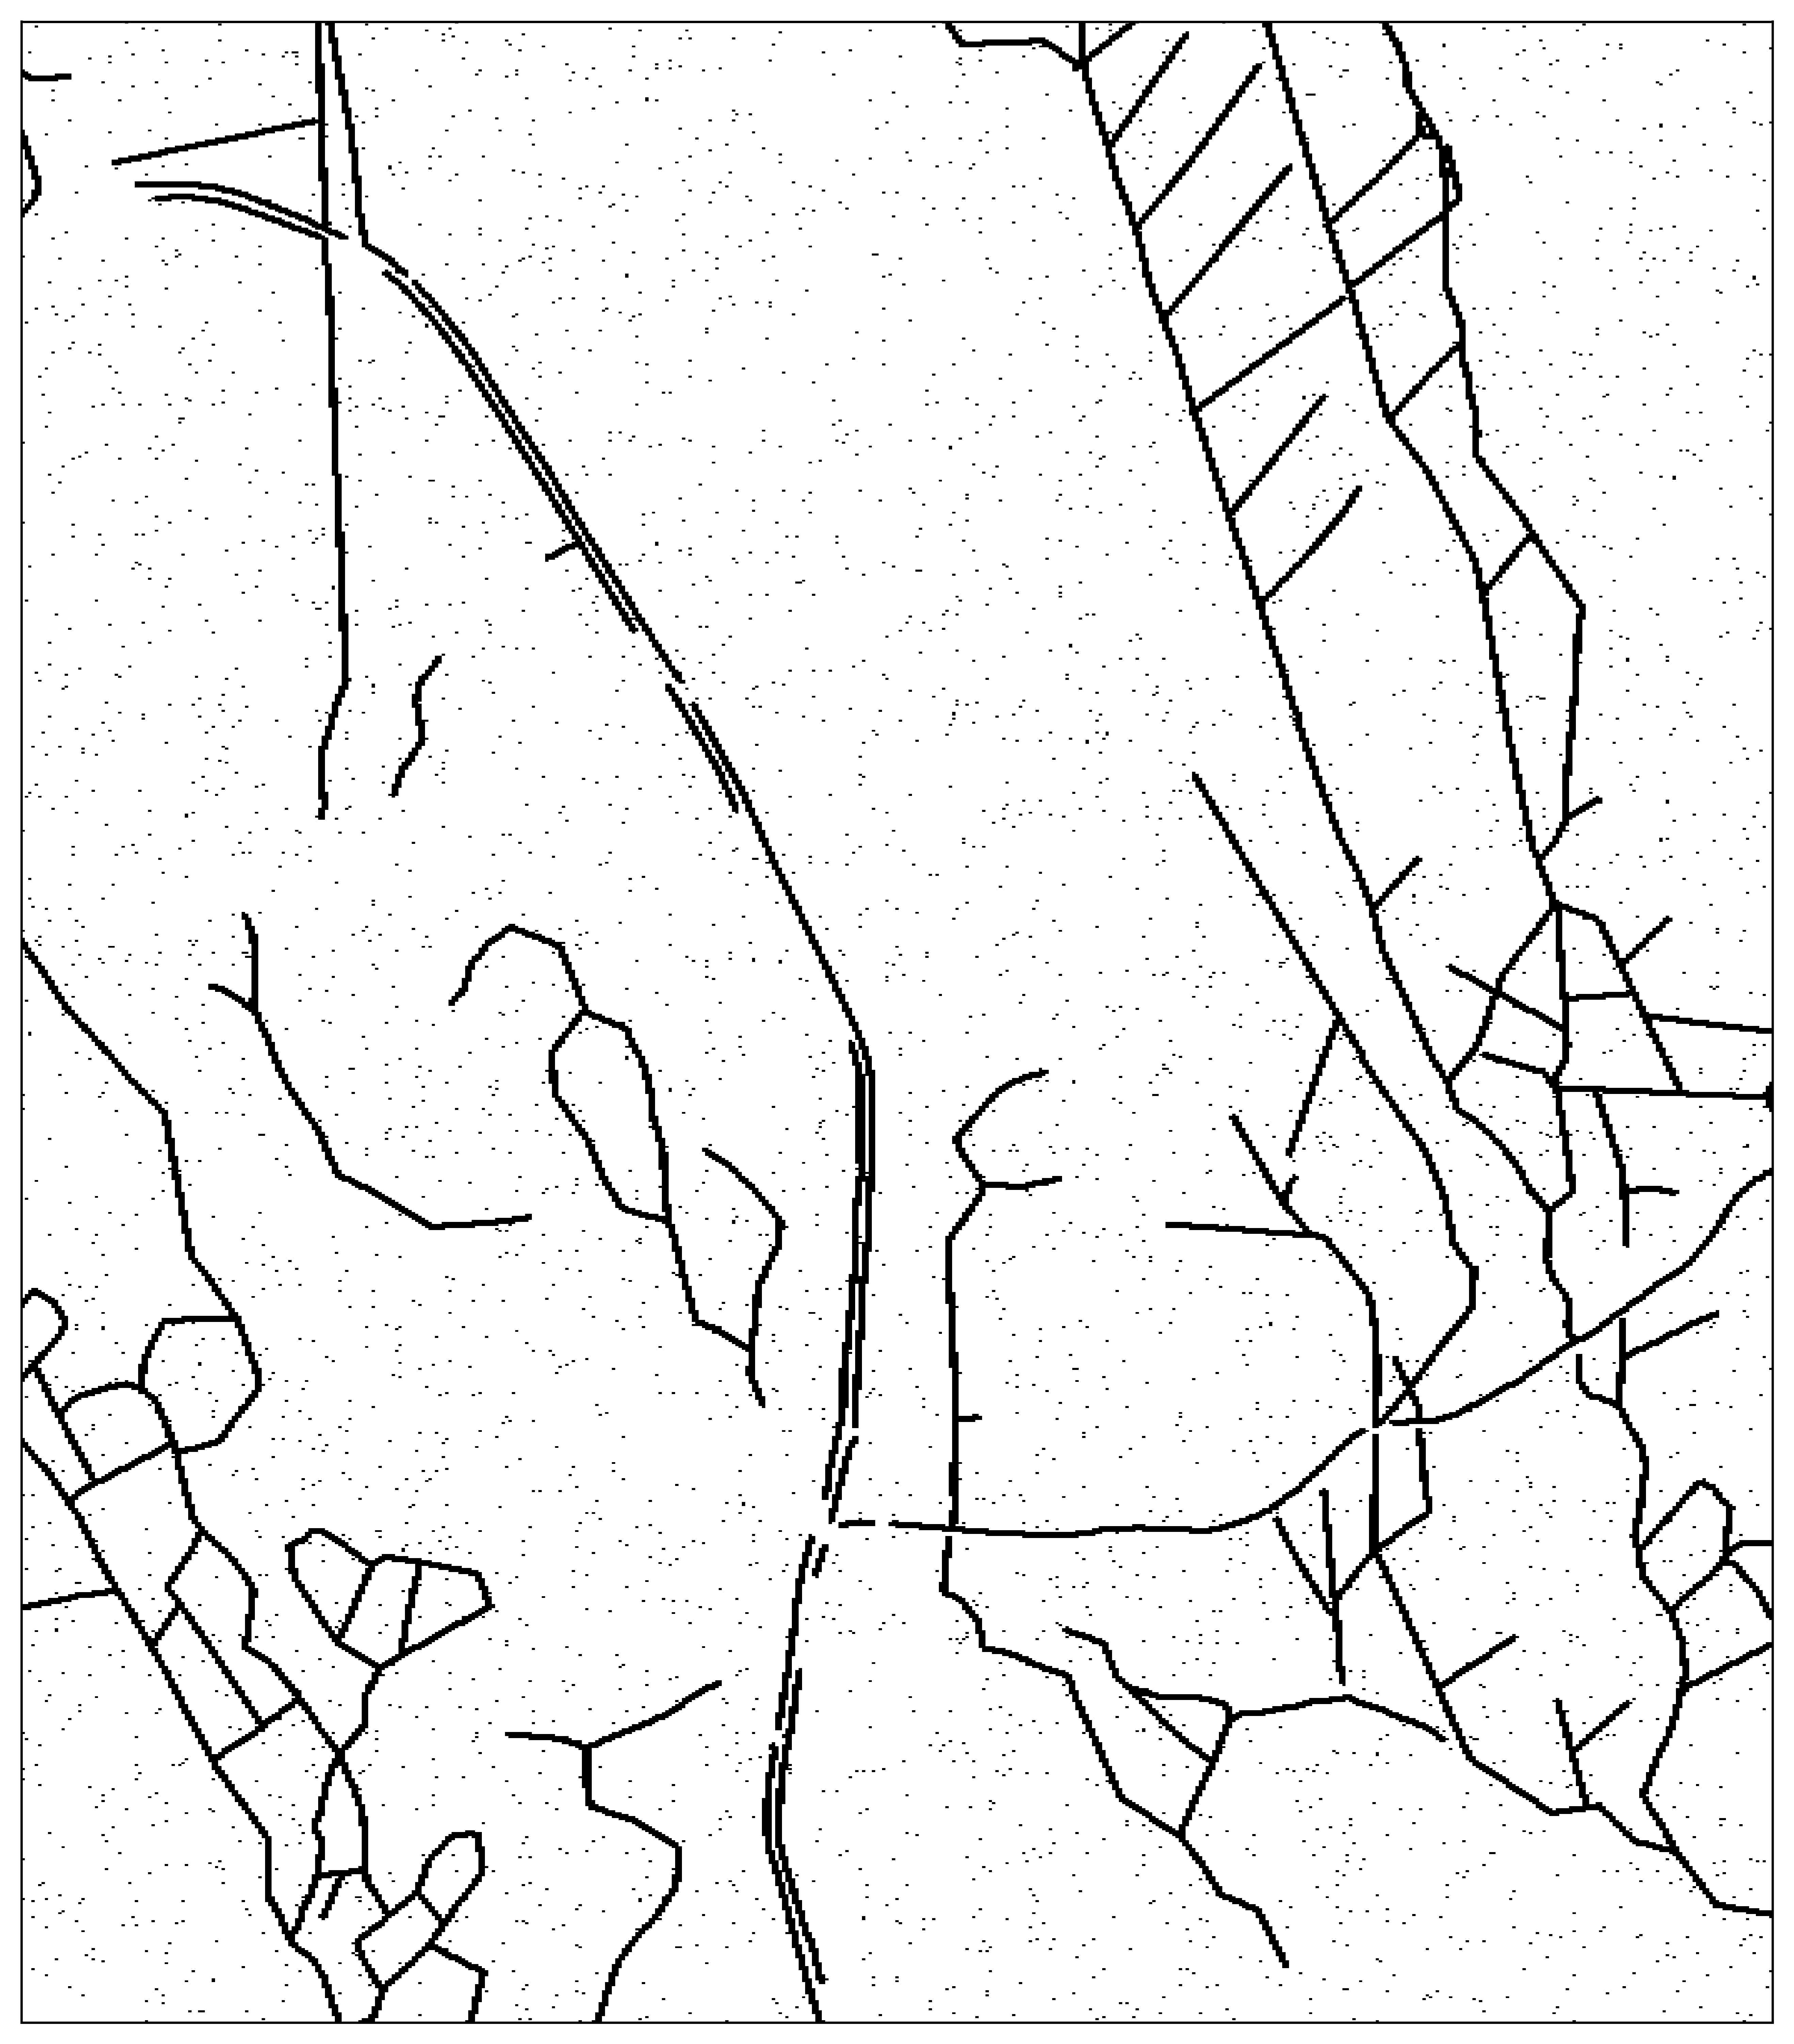
\includegraphics{./images/publ_balanced_masks_B_lo.jpg}}}
    \caption{\textbf{Balancing training data.} Black pixels here indicate the balanced masks used to determine what pixels were used when training the models. \textbf{a, b: }Examples of two subsection from the training dataset.}
    \label{fig:balancedmasks}
\end{figure}

\newpage
\subsection{Post-processing}

The output from the model is a ditch probability ranging from zero to one for each pixel (\hyperref[fig:postprocessing1]{Figure} \ref{fig:postprocessing1} \hyperref[fig:postprocessing1]{a}).

\subsubsection{Noise reduction and gap filling}

The probability predictions contained a lot of noise in the areas largely distant from the ditches. This noise was removed by first using a bilateral de-noising filter, and then removing outlier pixels that were far away from any other high probability ditch pixels. This left linear properties and pixels with a very high value intact, while lowering the value of pixels that did not contribute to an accurate prediction (\hyperref[fig:postprocessing1]{Figure} \ref{fig:postprocessing1} \hyperref[fig:postprocessing1]{b}) (\hyperref[fig:postprocessing2]{Figure} \ref{fig:postprocessing2} \hyperref[fig:postprocessing2]{a}).

To fill gaps in ditches that the model failed to correctly predict due to gaps in the LiDAR scans, we aggregated pixel values by covering them with cone masks expanding outwards in different directions from the examined pixel. This amplified some of the noise that was left, but filling the gaps in the ditches was judged to be more important (\hyperref[fig:postprocessing2]{Figure} \ref{fig:postprocessing2} \hyperref[fig:postprocessing2]{b}).

\begin{figure} [!htb]
    \centering
    \subfigure[]{
        \resizebox*{5.6cm}{!}{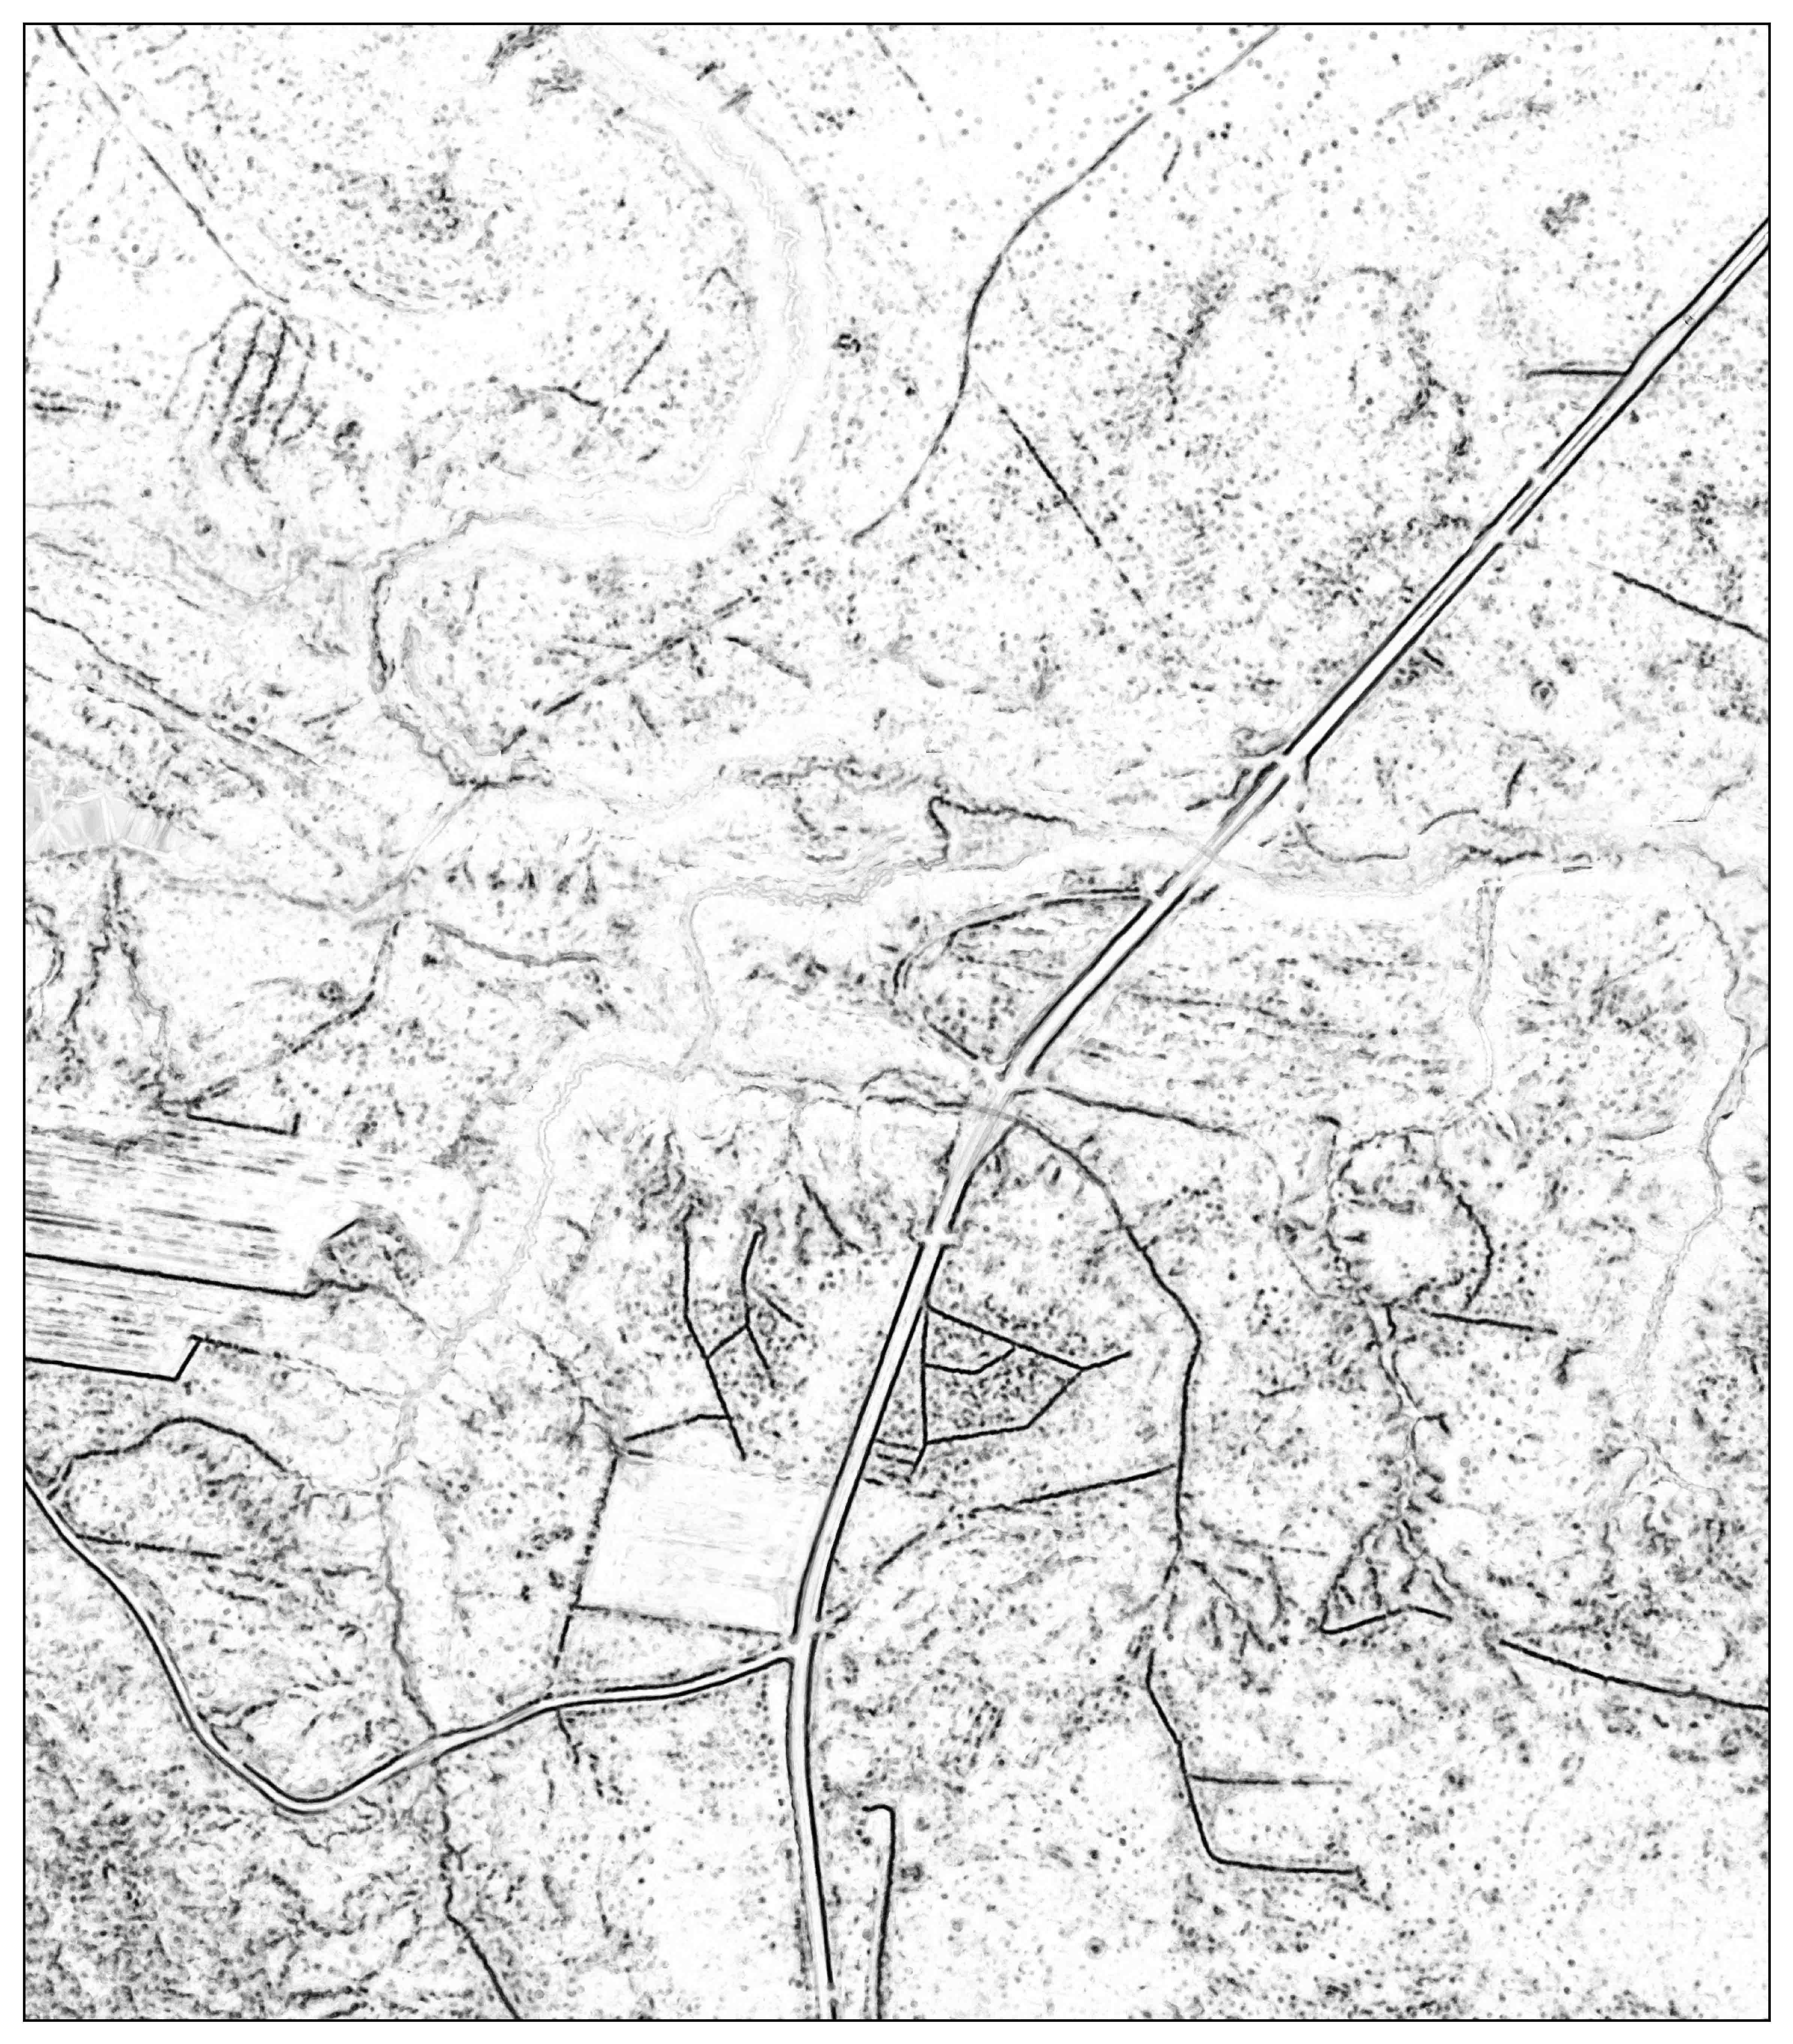
\includegraphics{./images/publ_post_process_step_1_lo.jpg}}}\hspace{5pt}
    \subfigure[]{
        \resizebox*{5.6cm}{!}{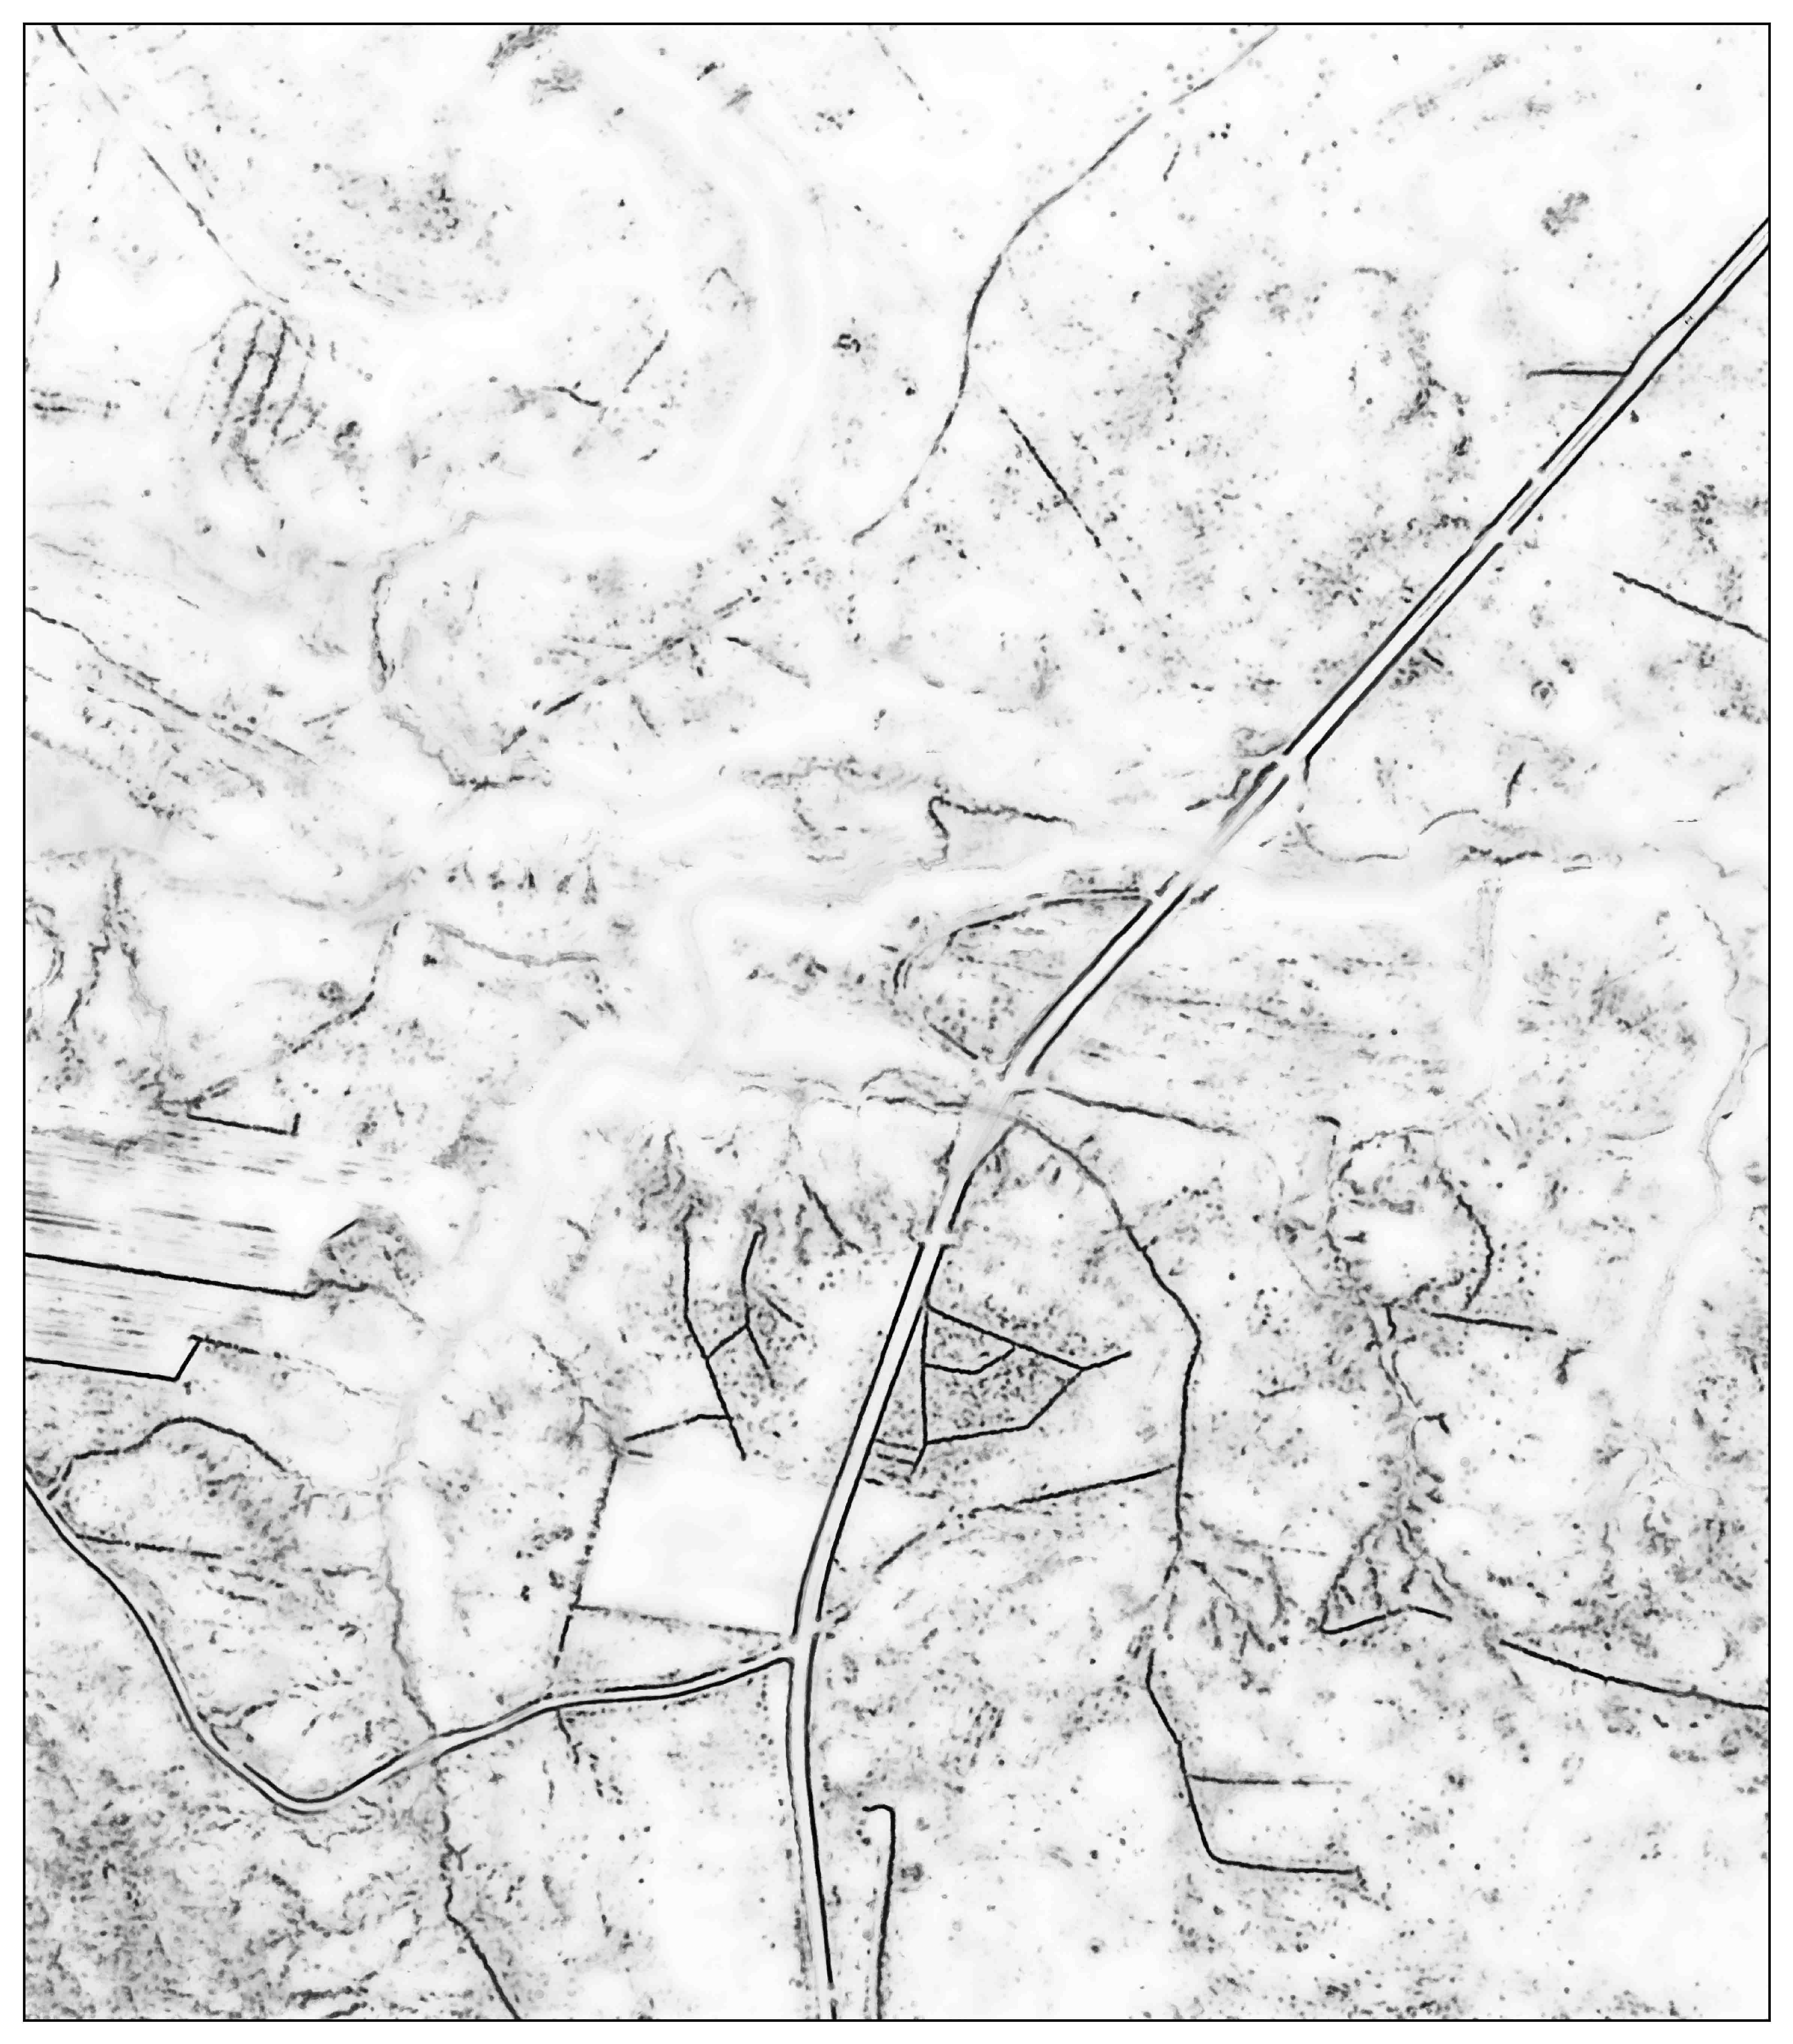
\includegraphics{./images/publ_post_process_step_2_lo.jpg}}}
    \caption{\textbf{Post-processing step one and two.} Darker pixels indicate a higher ditch probability. \textbf{a: }Random Forests probability prediction. \textbf{b: }Bilateral de-noising.}
    \label{fig:postprocessing1}
\end{figure}

\begin{figure} [!htb]
    \centering
    \subfigure[]{
        \resizebox*{5.6cm}{!}{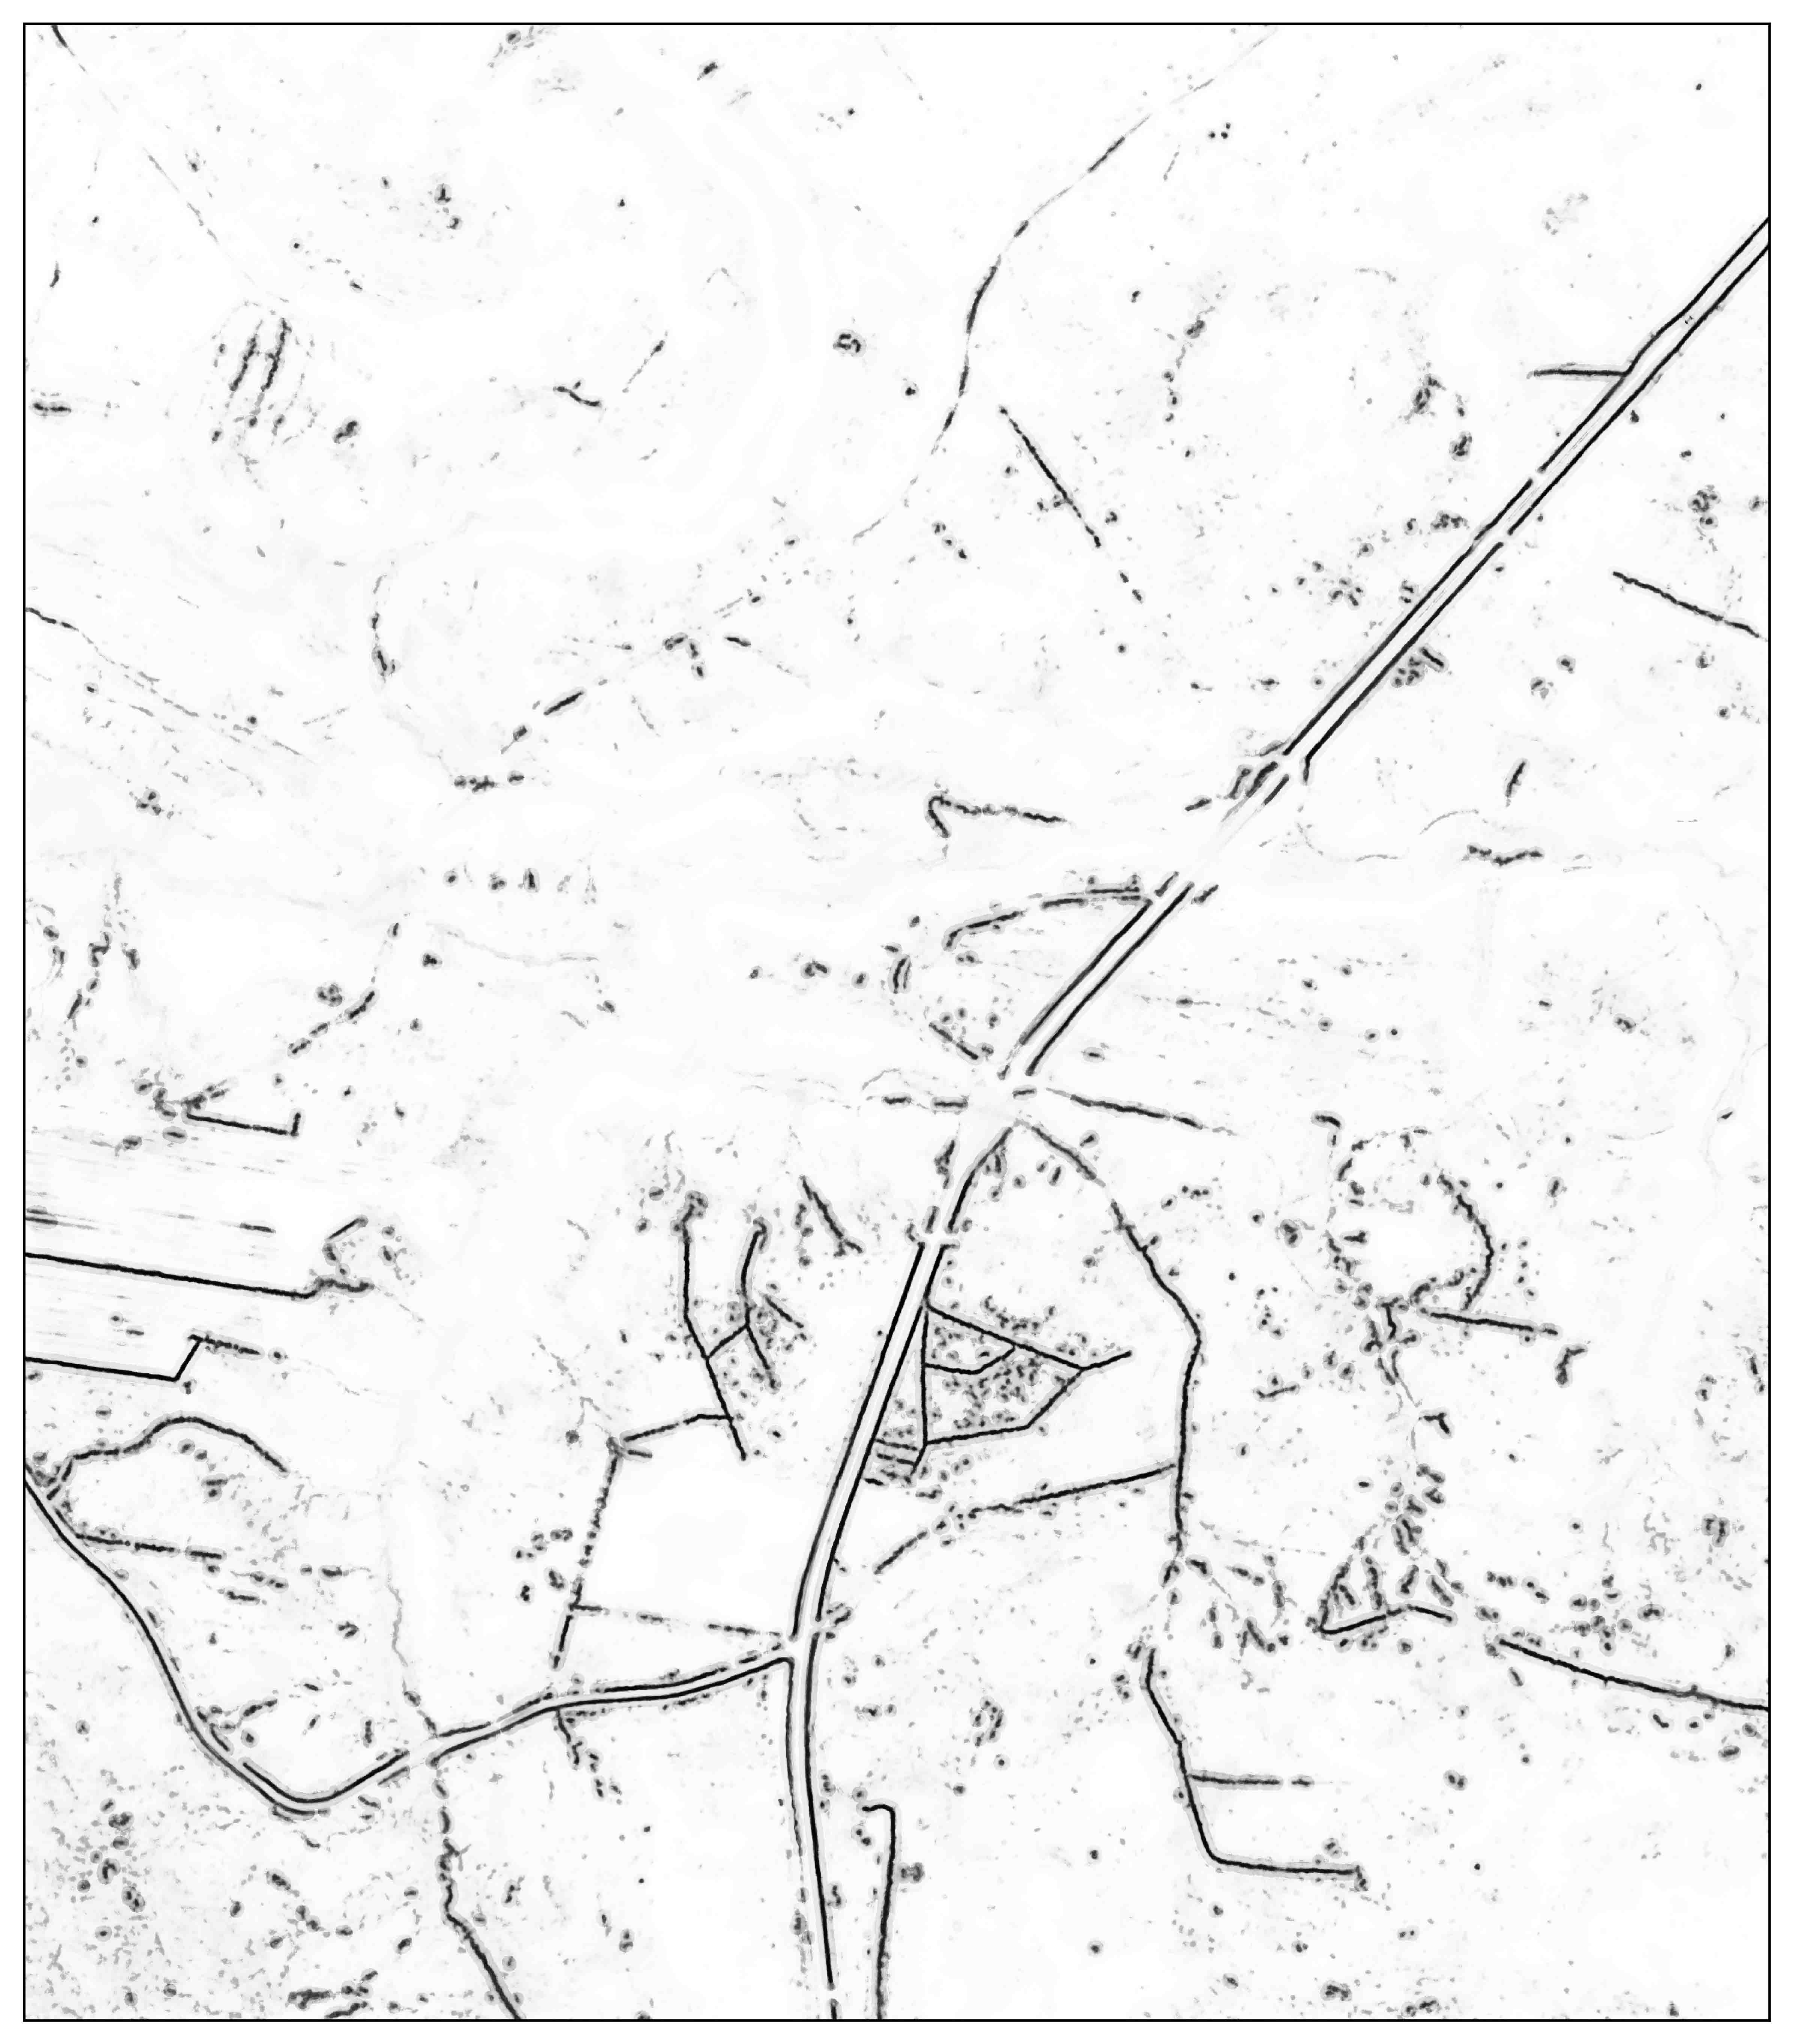
\includegraphics{./images/publ_post_process_step_3_lo.jpg}}}\hspace{5pt}
    \subfigure[]{
        \resizebox*{5.6cm}{!}{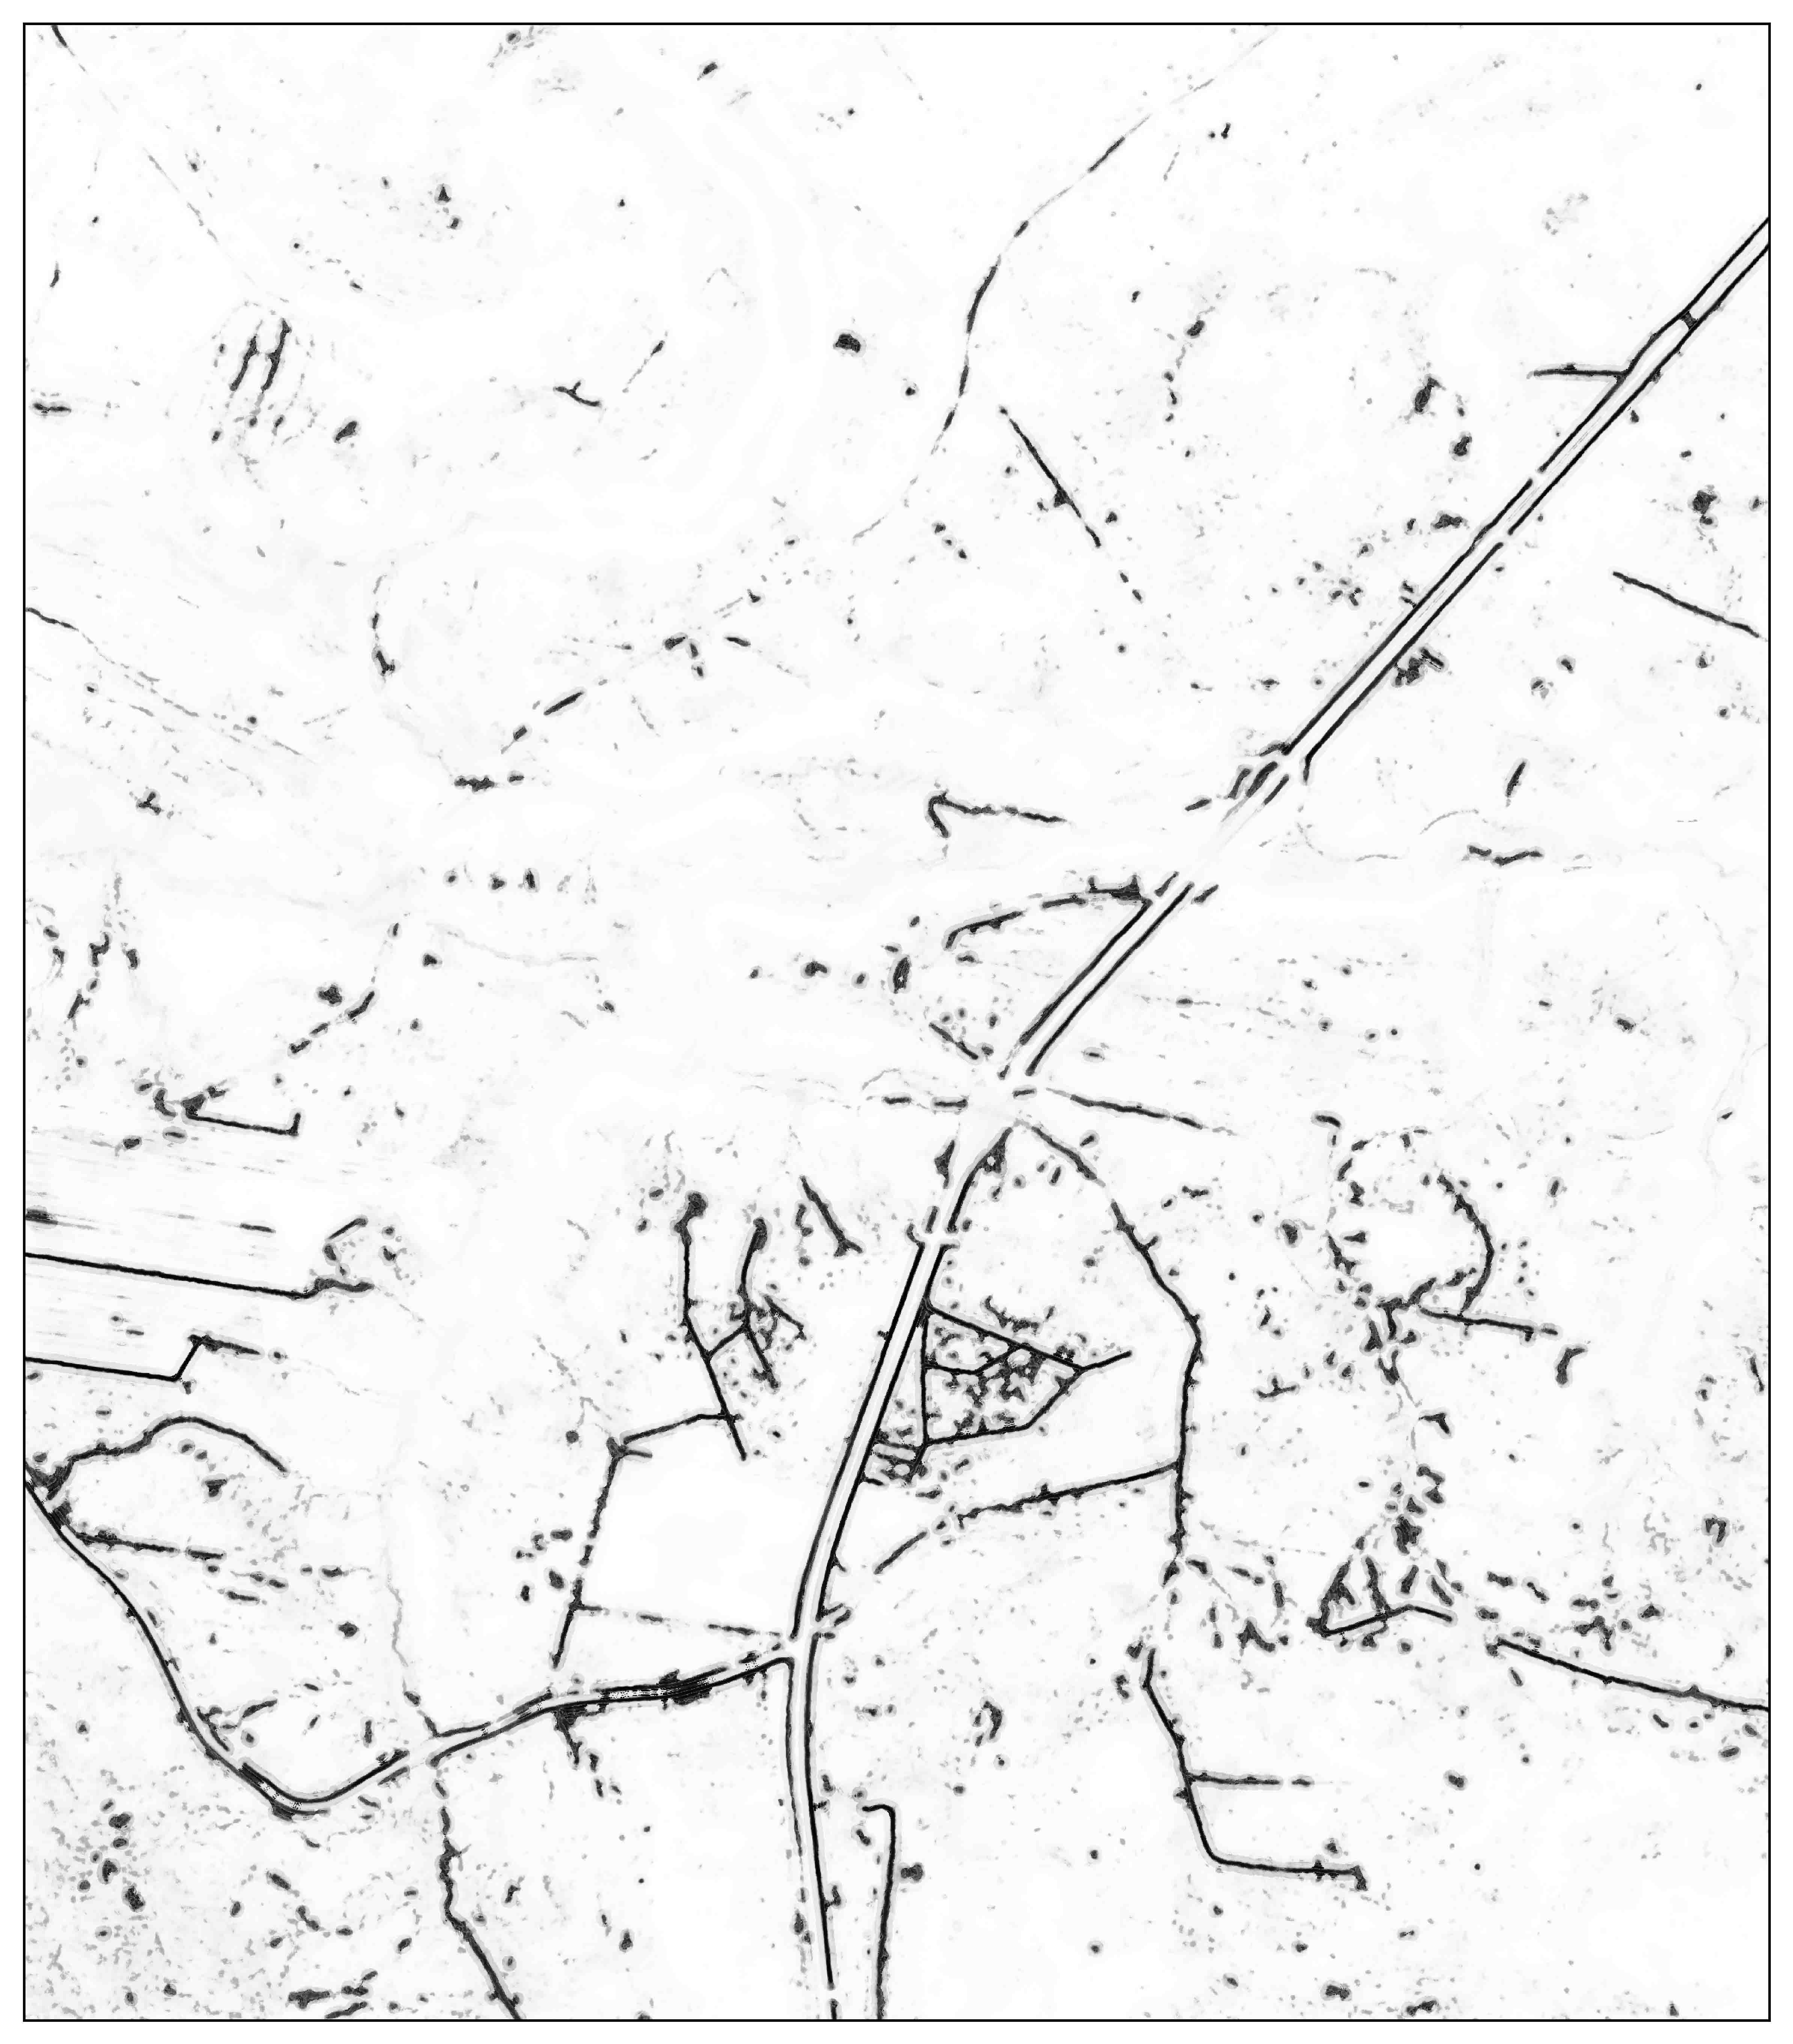
\includegraphics{./images/publ_post_process_step_4_lo.jpg}}}
    \caption{\textbf{Post-processing step three and four.} Darker pixels indicate a higher ditch probability. \textbf{a: }Custom de-noising. \textbf{b: }Gap filling.}
    \label{fig:postprocessing2}
\end{figure}

\subsubsection{Binarisation and cluster removal}

To correct errors where lone pixels inside ditches had been incorrectly classified, the resolution was lowered by binary classifying each $6*6$ pixel grid as a ditch or a non-ditch if the mean probability of the pixels inside the grid exceeded 40 \% (\hyperref[fig:postprocessing3]{Figure} \ref{fig:postprocessing3} \hyperref[fig:postprocessing3]{a}). The same zone partitioning was performed on the labels (\hyperref[fig:ditchpreprocess]{Figure} \ref{fig:ditchpreprocess} \hyperref[fig:ditchpreprocess]{c}).

A cluster detection algorithm was developed to remove noise from the final ditch prediction. By finding the number of connected pixels with a true value and removing those whose cluster size were below a threshold, minor noise in the prediction could be removed while still retaining most of the ditch pixels. A distance calculation was also performed in tandem with this method to find the largest distance of pixels inside each given cluster. This helped to remove sinks and hollows that were not removed by the initial small cluster removal, but that did not have a linear directional characteristic, indicating that they did not represent a ditch (\hyperref[fig:postprocessing3]{Figure} \ref{fig:postprocessing3} \hyperref[fig:postprocessing3]{b}).

\begin{figure} [!htb]
    \centering
    \subfigure[]{
        \resizebox*{5.6cm}{!}{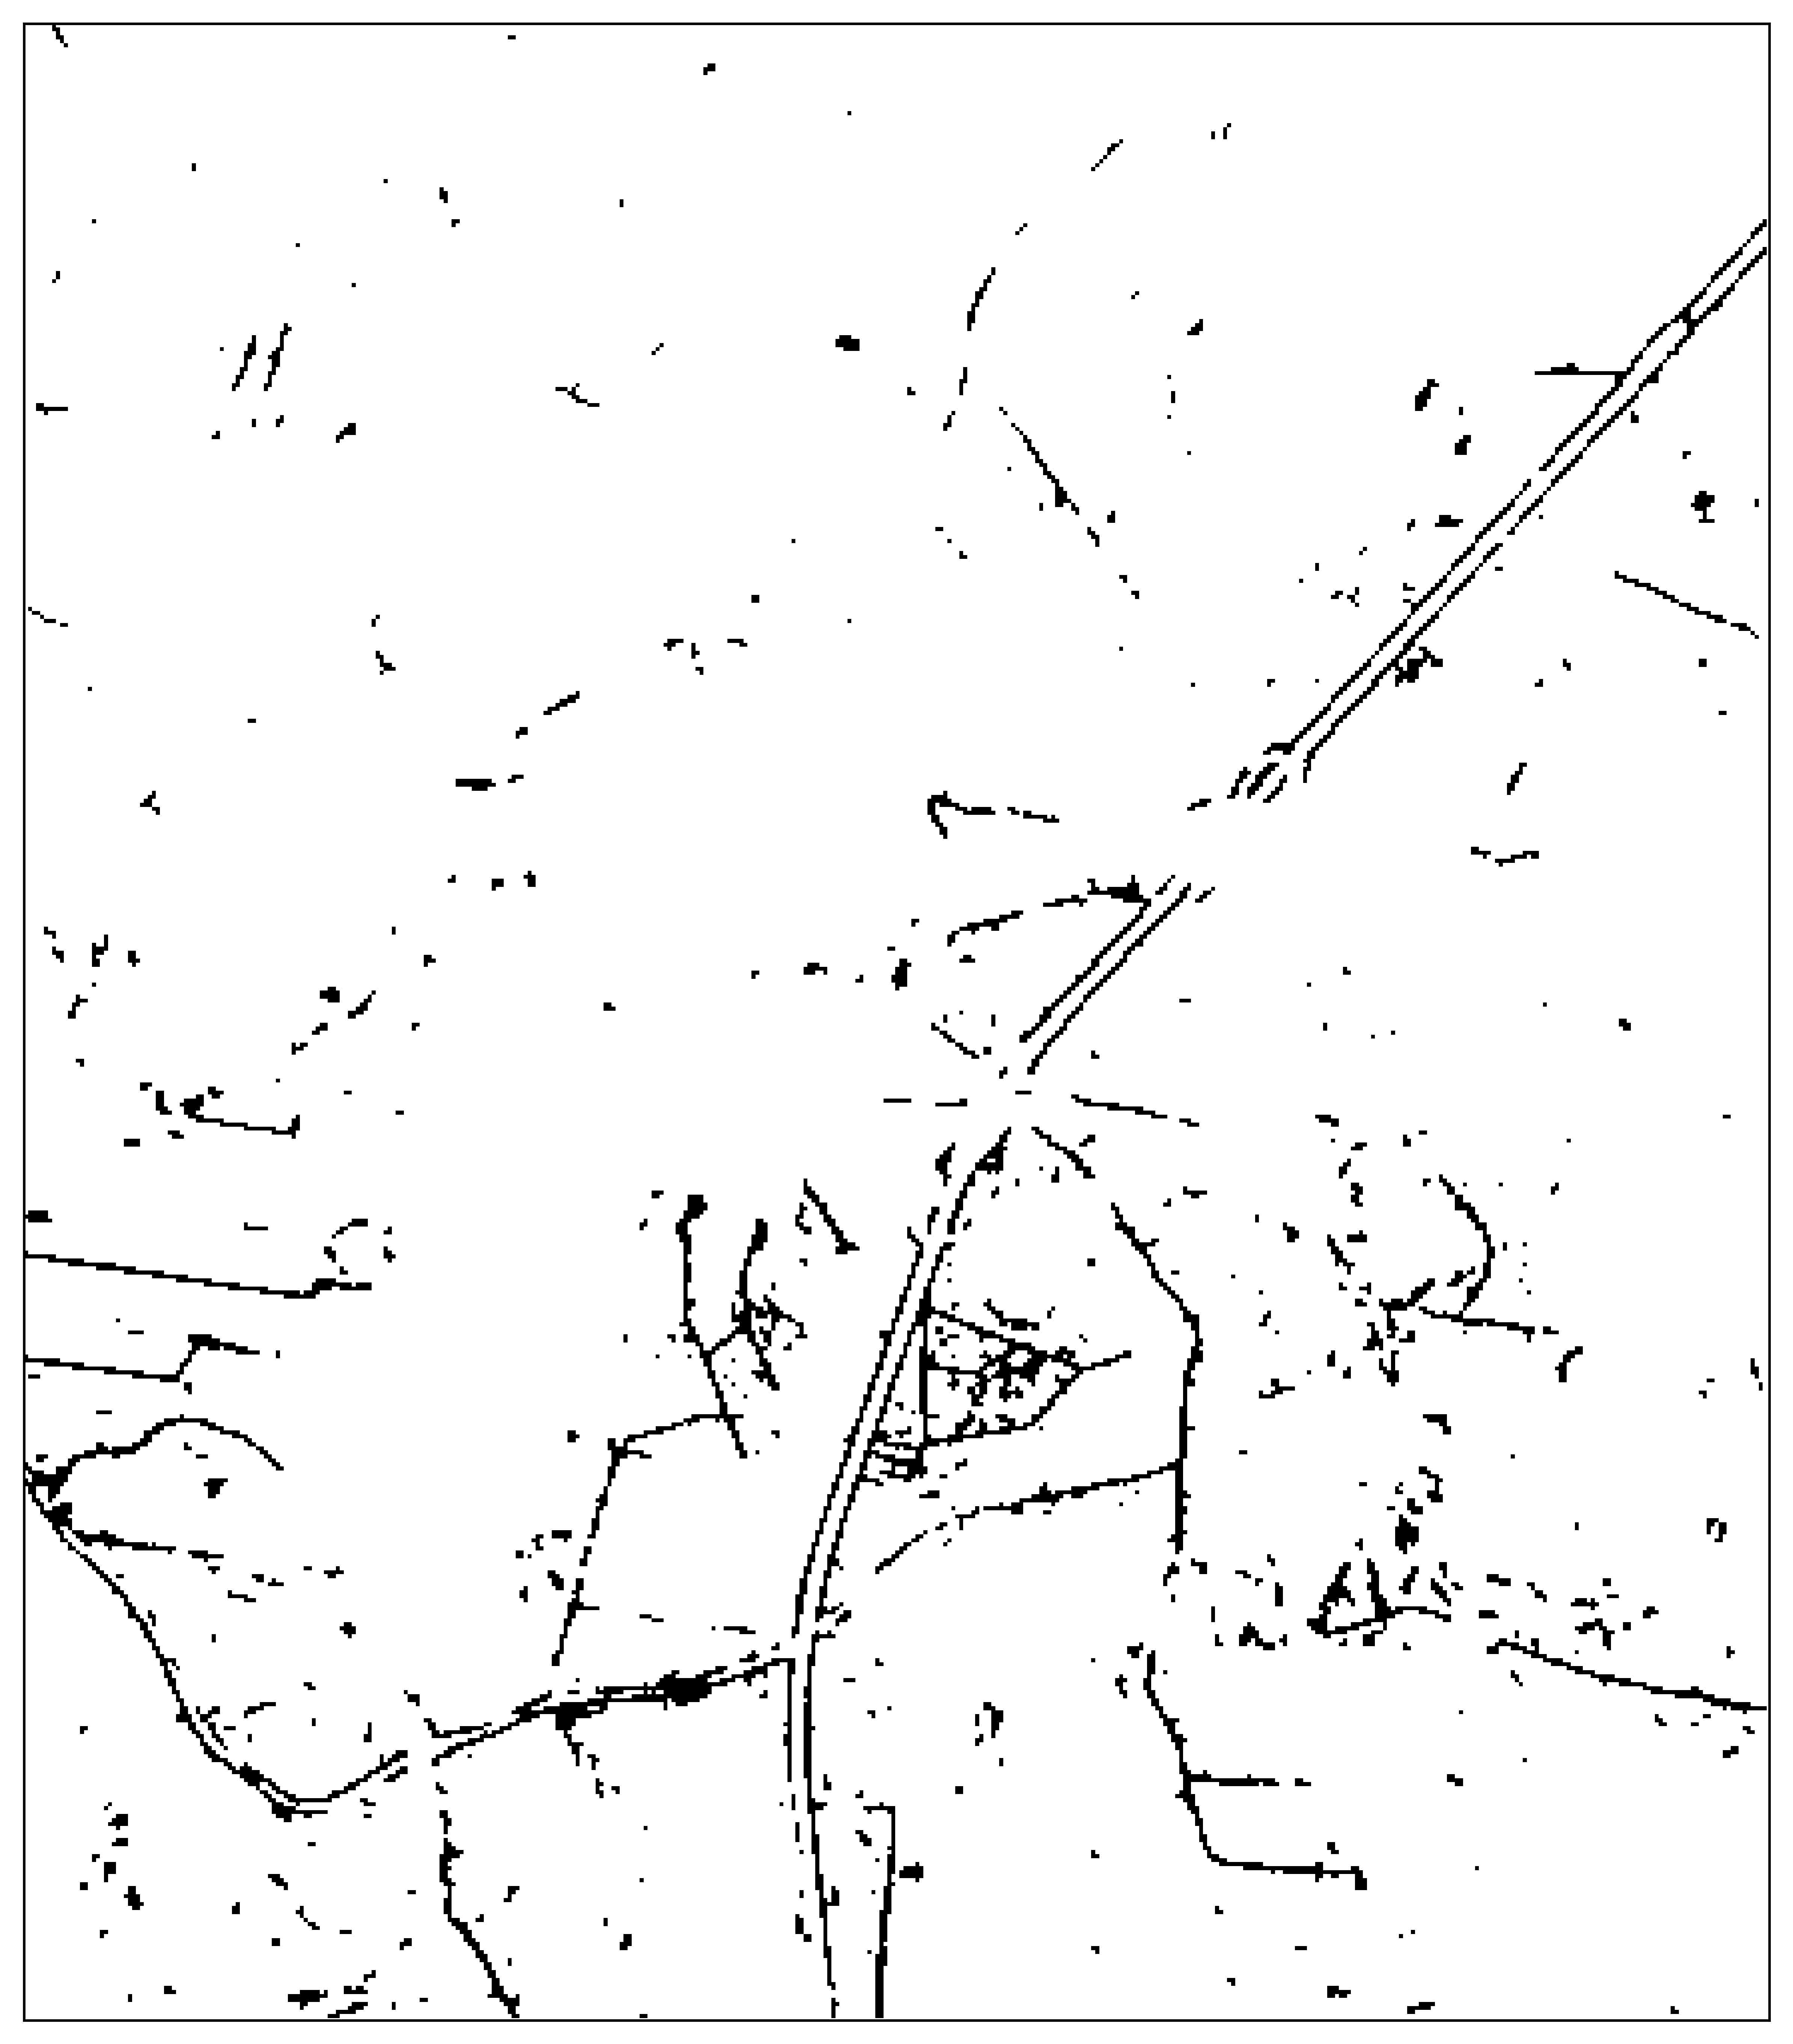
\includegraphics{./images/publ_post_process_step_5_lo.jpg}}}\hspace{5pt}
    \subfigure[]{
        \resizebox*{5.6cm}{!}{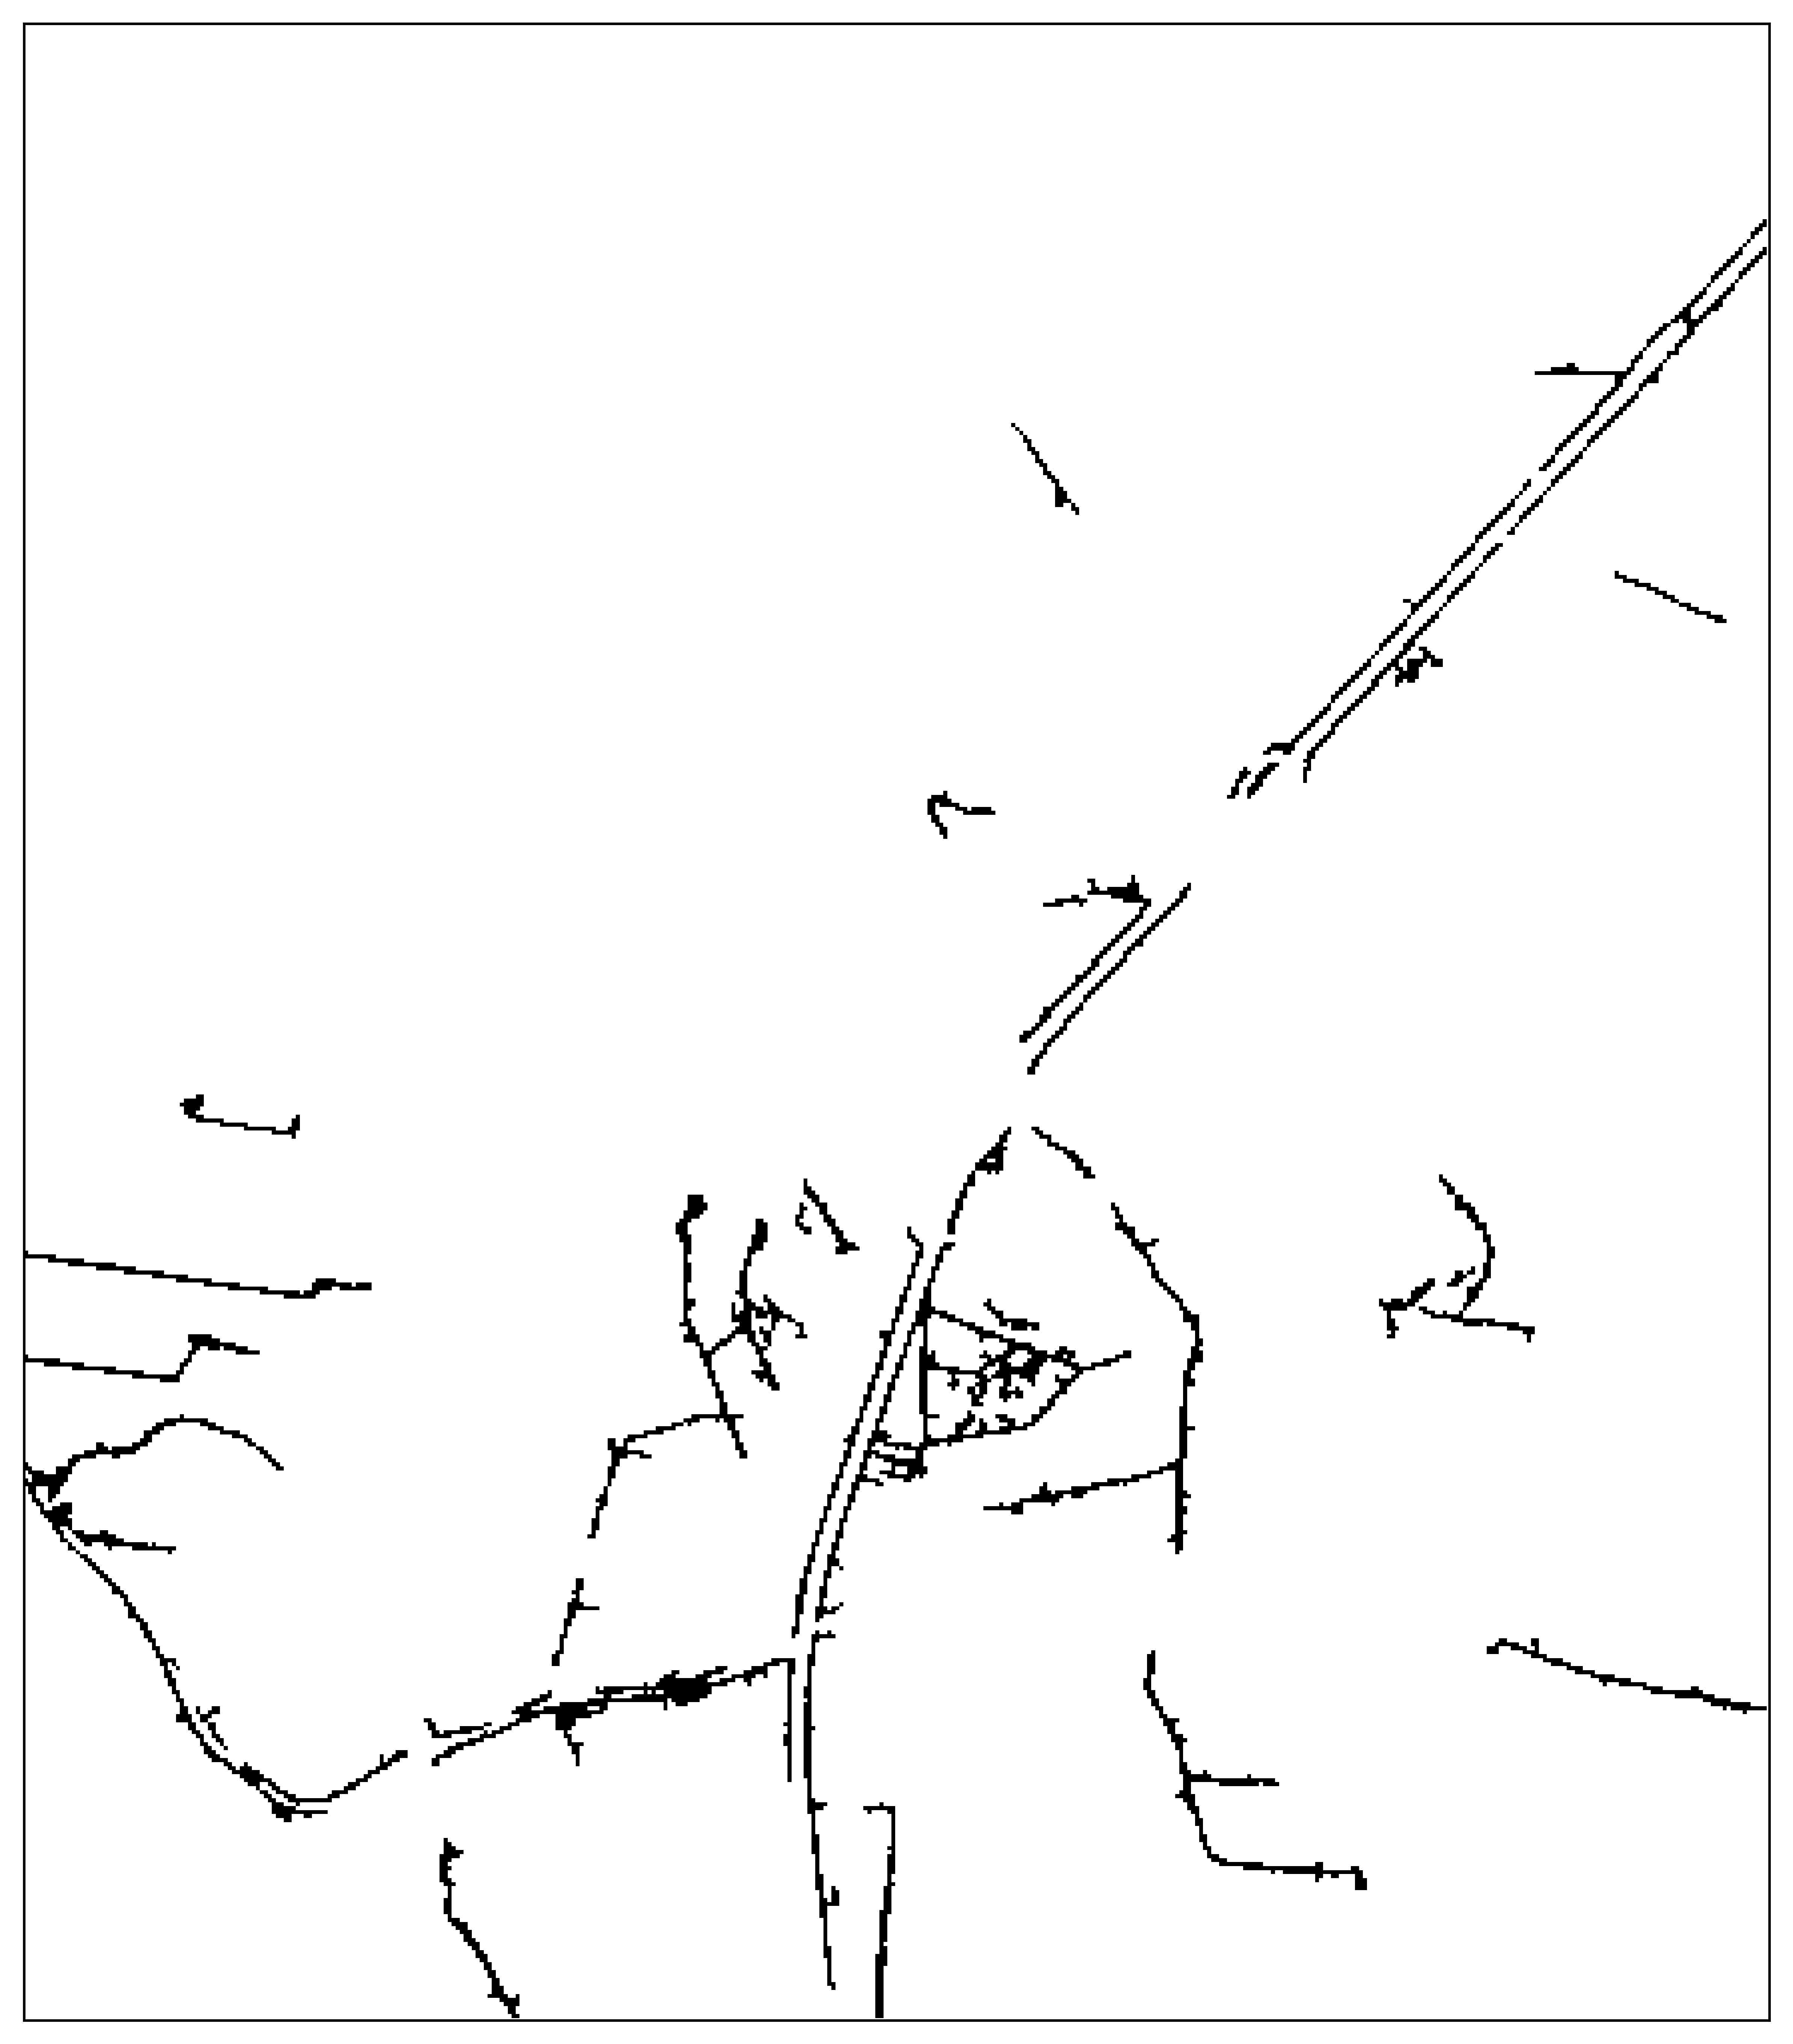
\includegraphics{./images/publ_post_process_step_6_lo.jpg}}}
    \caption{\textbf{Post-processing step five and six.} Black pixels indicate a ditch prediction. \textbf{a: }Grid zone binarisation \textbf{b: }Cluster removal (final ditch prediction).}
    \label{fig:postprocessing3}
\end{figure}

\subsection{Evaluation} \label{evaluation}

Using only accuracy as an evaluation metric when dealing with an imbalanced dataset (roughly 98 \% of all pixels are non-ditch) would produce a poor performance assessment \citep{balanced}; by simply classifying all pixels as non-ditches, we would by default attain 98 \% accuracy. For this reason, the results were mainly evaluated using Cohen's Kappa (Cohen's $\kappa$) index, and the Area under Precision-Recall curve. Cohen's $\kappa$ index measures how much better a prediction is compared to a completely random prediction, where predicting 2 \% of the occurrences as ditch pixels completely at random would yield a value of zero \citep{kappa123}. Values above zero are better than random, and values below zero are worse than random.

The random rating $P_c$ of a prediction of $n$ occurrences is calculated with:\footnote{ P = Positive (ditch pixel), N = Negative (non-ditch pixel), T = true, F = false}

$$
P_c = \frac{\left(\frac{(TP + FN) \cdot (TP + FP)}{n}\right) + \left(\frac{(FN + TN) \cdot (FP + TN)}{n}\right)}{n}
$$


Cohen's $\kappa$ is then calculated as a value between -1 and 1 with:

$$\kappa = \frac{Accuracy - P_c}{1 - P_c}$$

The Precision-Recall curve and the Area under Precision-Recall curve (AUPRC) are additional metrics that can be used when evaluating datasets with a largely imbalanced class distribution \citep{precision_recall_curve}. The weighting causes the Precision-Recall curve to place an unequal weight on true negatives and true positives \citep{precision_recall_curve}. For our ditch detection problem, this means that the AUPRC evaluation metric favours accurately classifying ditch pixels over accurately classifying non-ditch pixels.

To circumvent some of the evaluation issues arising from the use of pixel classification for ditch objects, as well as not having completely accurate labels on a pixel basis (due to uncertainties in the width of the ditches), we modified the evaluation labels to allow for some error in close proximity to ditches in the prediction. False negative and false positive grid zones that lay adjacent to the ditch label grid zones were evaluated as true negatives and true positives, as they can be considered a part of correctly located ditch objects (\hyperref[fig:newlabels]{Figure} \ref{fig:newlabels}).

\begin{figure} [!htb]
    \centering
    \subfigure[]{
        \resizebox*{6.65cm}{!}{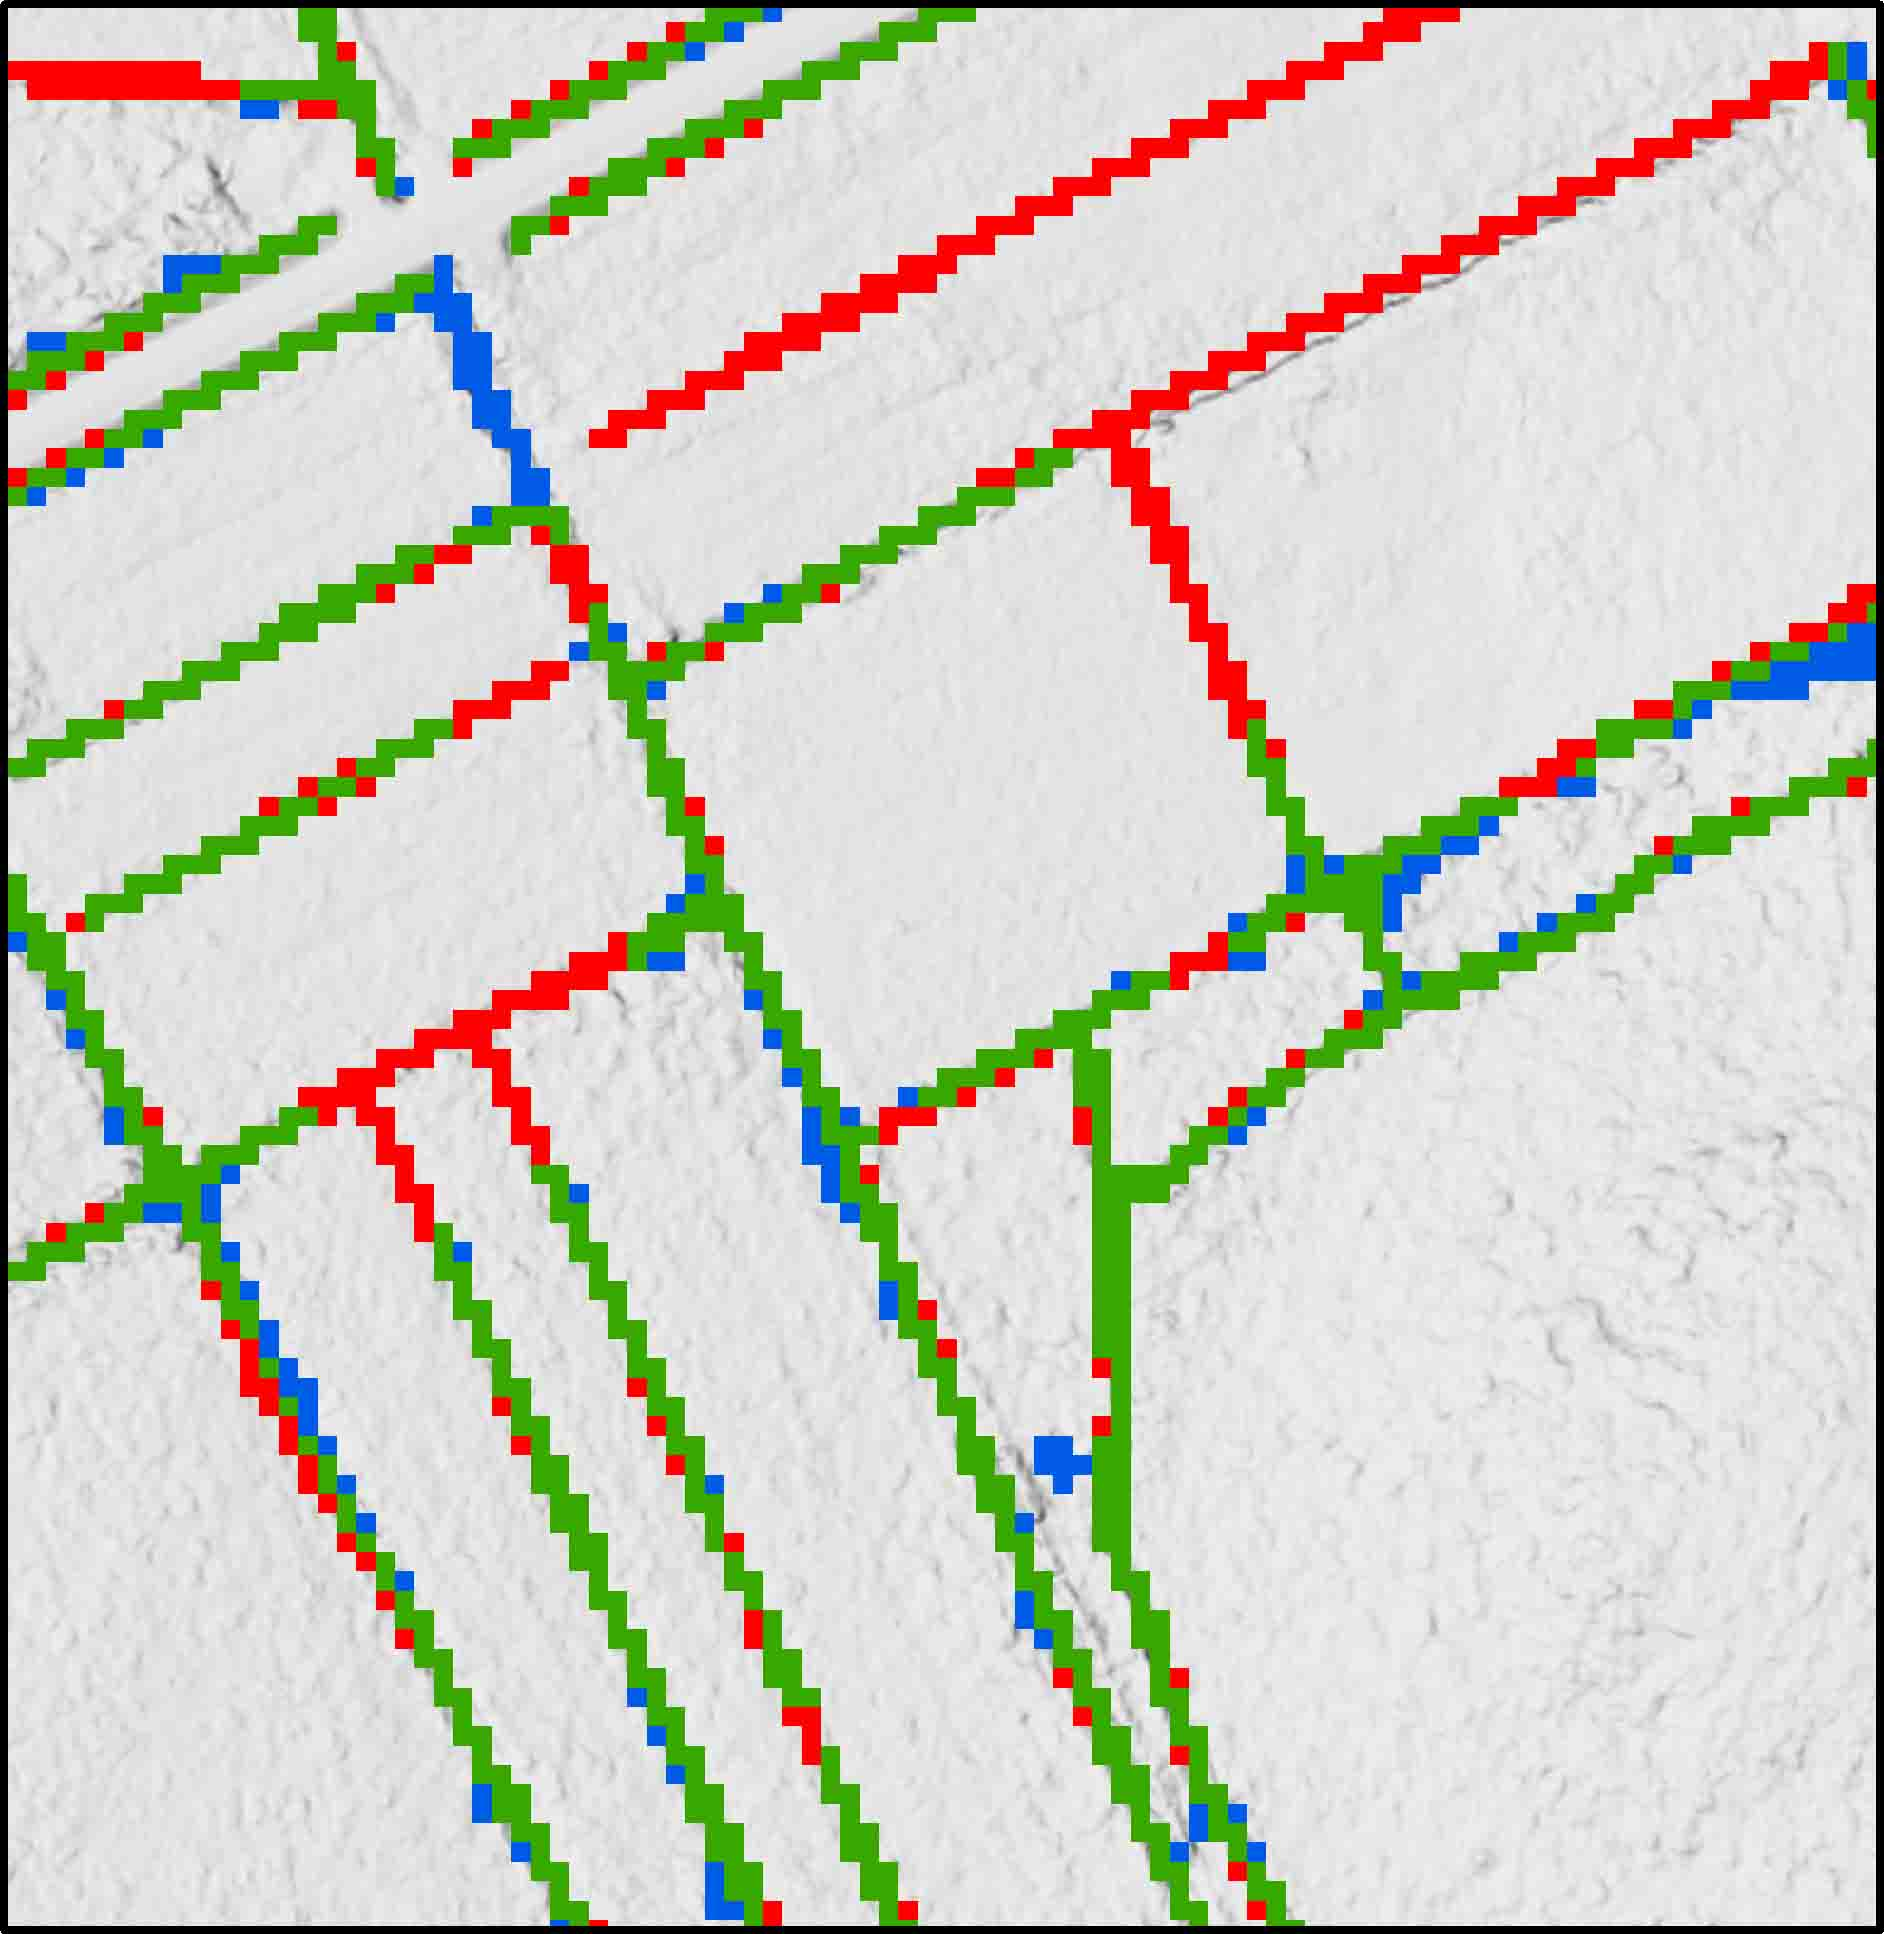
\includegraphics{./images/re_evaluation_1_lo.jpg}}}\hspace{5pt}
    \subfigure[]{
        \resizebox*{6.65cm}{!}{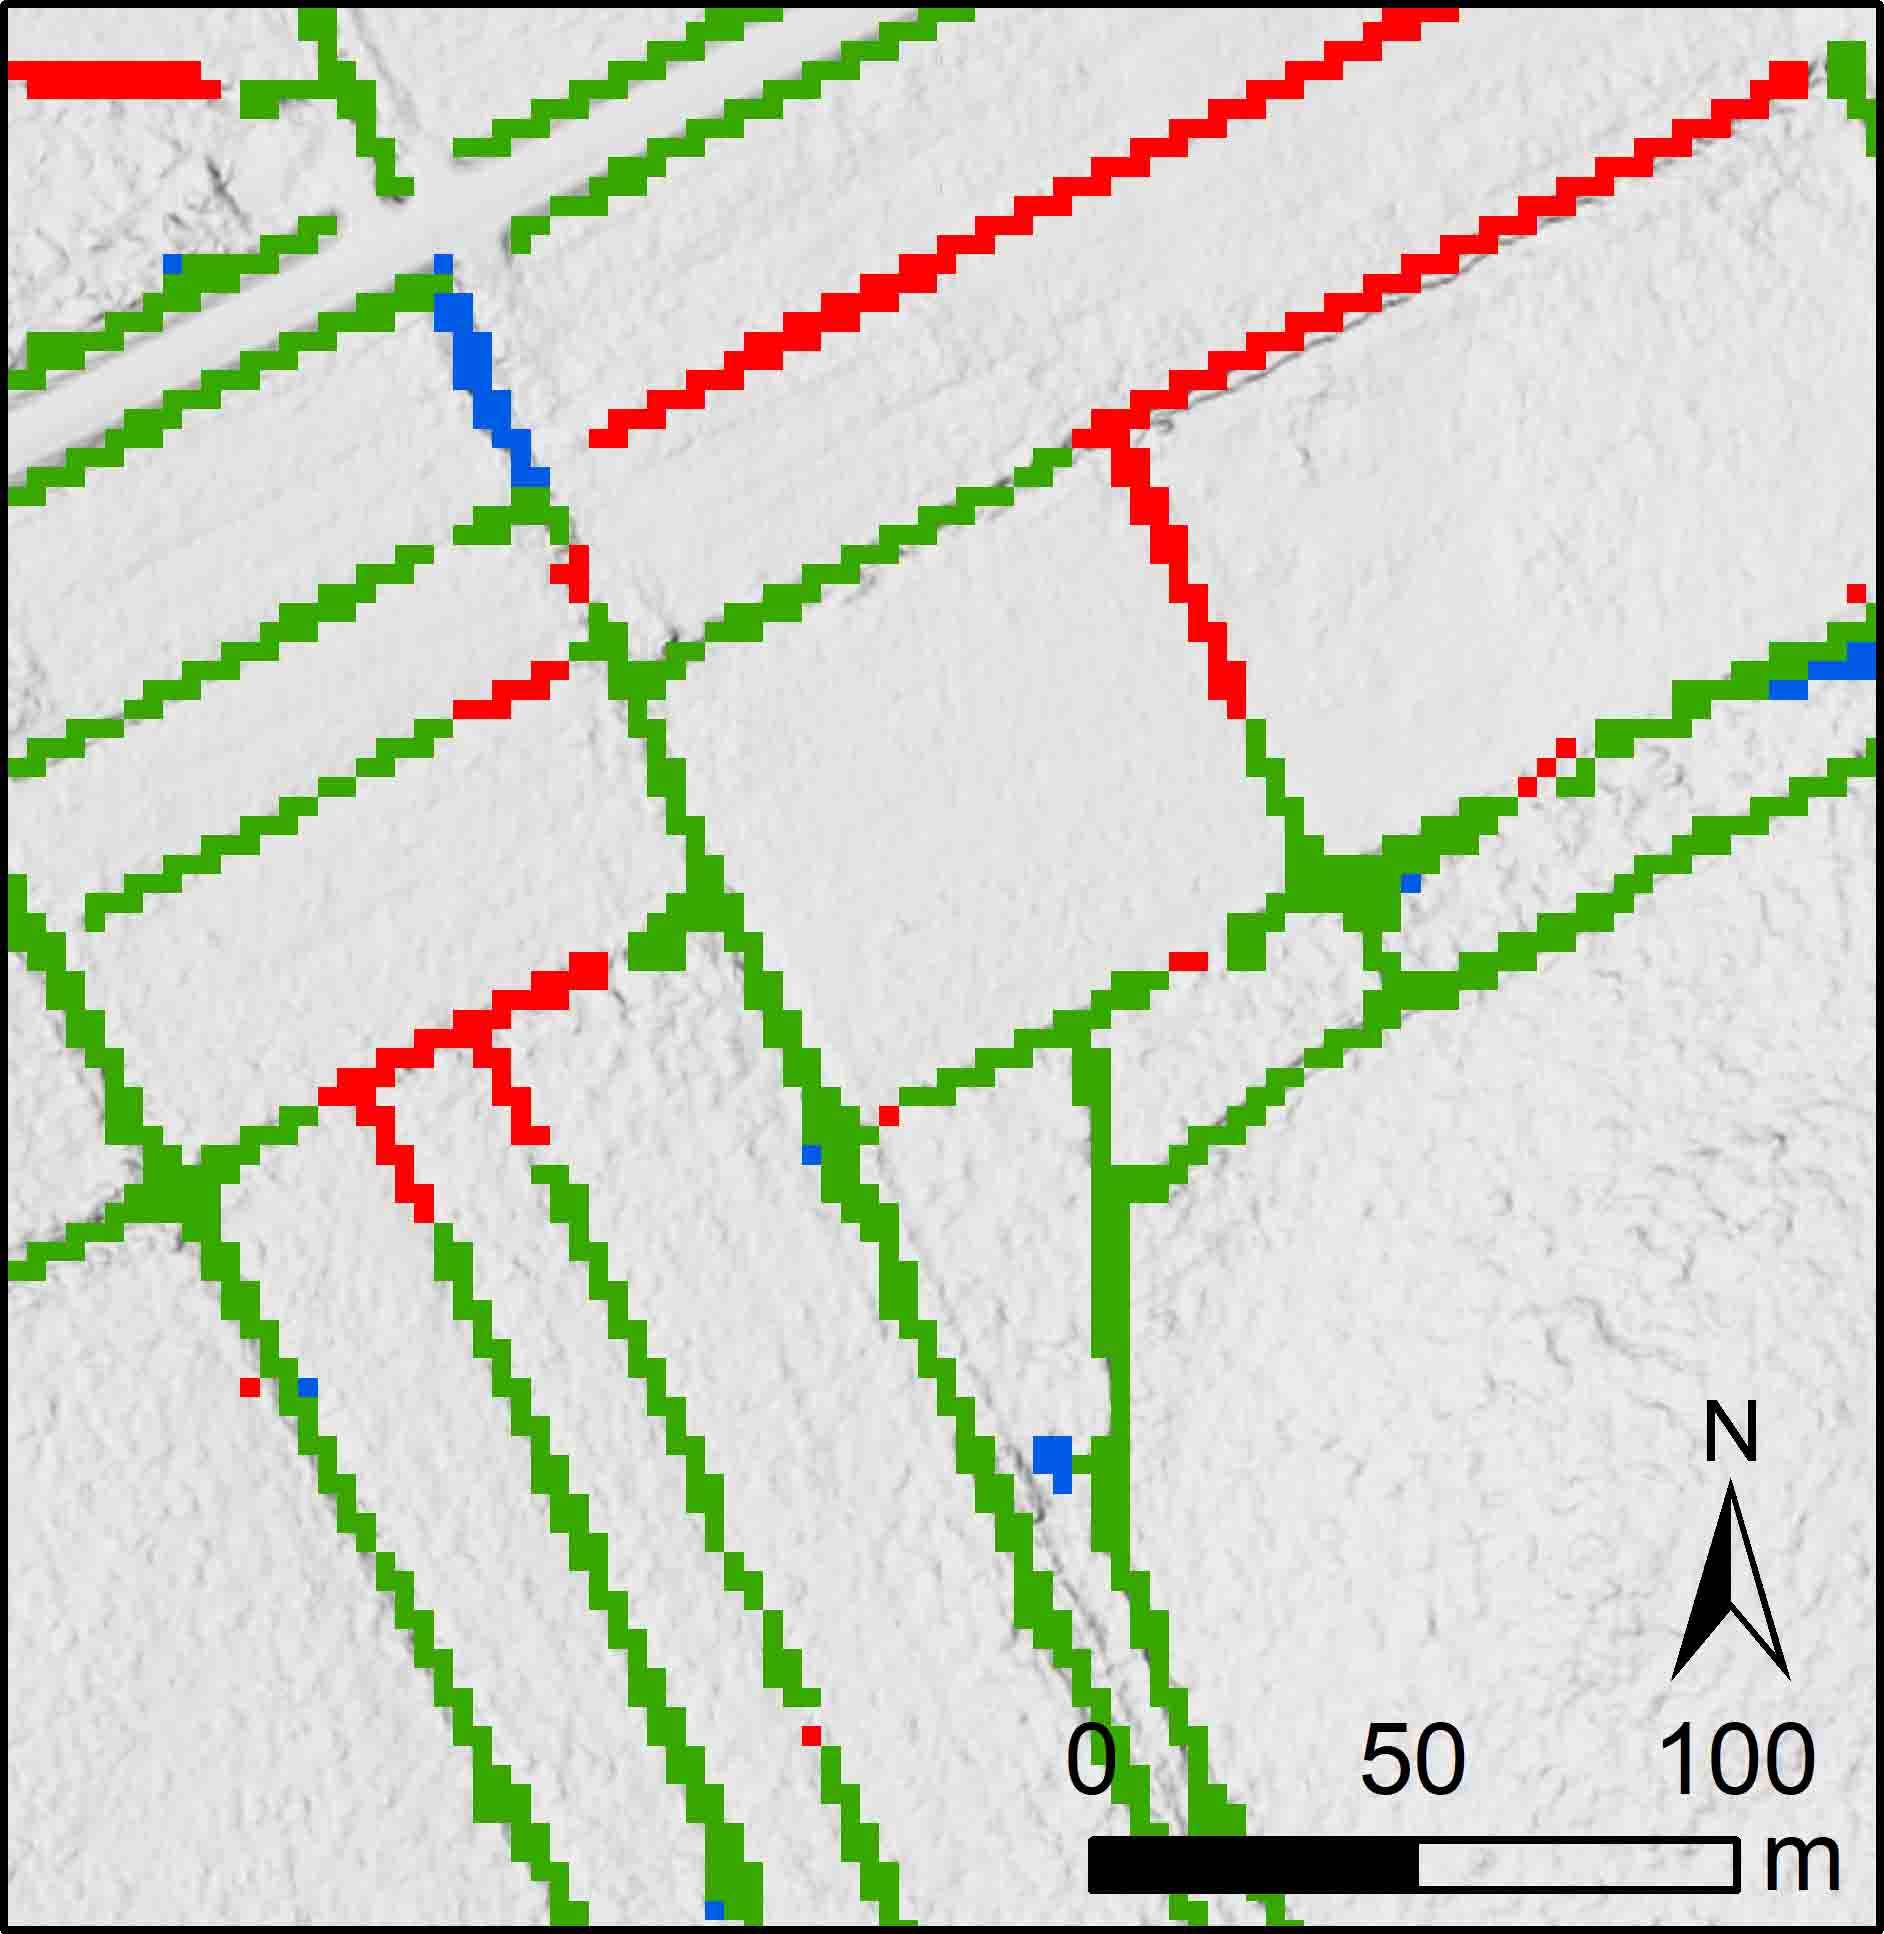
\includegraphics{./images/re_evaluation_2_lo.jpg}}}
    \caption{\textbf{Modifying evaluation labels.} Green marks true positives, red marks false negatives, and blue marks false positives. False positives and false negatives that lay within one grid zone (9 $m^2$) of a ditch label were evaluated as true positives and true negatives. \textbf{a:} Original results, \textbf{b:} Modified results. }
    \label{fig:newlabels}
\end{figure}

\section{Results and analysis}

\hyperref[recreatedpredictionperformance]{Table} \ref{recreatedpredictionperformance} shows the evaluation metrics from the experiments where the digital terrain indices were thresholded separately. Of the four, the \hyperref[impoundment]{Impoundment Index} and \hyperref[hpmf]{HPMF} performed relatively close to each other, and outperformed the other indices for most of the metrics.

\begin{table}[!htb]
\centering
    {\begin{tabular}{lcccc}
        \textbf{Metric} & \textbf{\hyperref[skyviewfactor]{Sky View Factor}} & \textbf{\hyperref[impoundment]{Impoundment}} & \textbf{\hyperref[hpmf]{HPMF}} & \textbf{\hyperref[slope]{Slope}}\\
        \hline
        Accuracy \%     & 83.67 & 97.07 & 97.45 & 82.66 \\
        Recall \%       & 44.54 & 29.98 & 25.31 & 34.83 \\
        Precision \%    &{ 4.00}  & 18.51 & 20.10 & { 2.99} \\
        $\kappa$ rating & 0.048 & 0.215 & 0.211 & 0.029 \\
        AUPRC & 0.247 & 0.248 & 0.232 & 0.194 \\
        \hline
    \end{tabular}}
    \caption{\textbf{Index thresholding metrics.} Metrics from the total results of the four digital terrain indices experiments, where only a sole terrain index is used with a threshold to detect ditches.}
    \label{recreatedpredictionperformance}
\end{table}

\hyperref[predictionperformance]{Table} \ref{predictionperformance} displays all the evaluation metrics for the prediction of our ditch detector. The confidence intervals were calculated from the results from the 11 cross-validation subsections. Because the subsections have varying amounts of ditches in them, the confidence intervals will not be completely conclusive, but will produce a close estimation. Averaging the results from the 11 subsections yields a very similar value to the total results, indicating that the ditch detector generally performs equally well on subsections with a small amount of ditches as on subsections with a large amount of ditches.

\begin{table}[!htb]
\centering
    {\begin{tabular}{lccc}
        \textbf{Metric} & \textbf{Total}\textsuperscript{a} & \textbf{Subsection Average}\textsuperscript{b}& \textbf{CI 95\%}\textsuperscript{c} \\ 
        \hline
        Accuracy     \% & 99.00 & 99.00 & [98.69 , 99.32] \\
        Recall       \% & 70.28 & 70.19 & [61.28 , 79.09] \\
        Precision    \% & 77.38 & 75.79 & [71.94 , 79.64] \\
        $\kappa$ rating & 0.732 & 0.718 & [0.655 , 0.781] \\
        AUPRC           & 0.741 & 0.733 & [0.674 , 0.791] \\
        \hline
    \end{tabular}}
    \caption{\textbf{Ditch detector performance metrics.} \newline
    \textsuperscript{a} The result of all 11 subsection experiments when combined. \newline
    \textsuperscript{b} An average score from the 11 different subsections that the experiment was performed on. \newline
    \textsuperscript{c} Confidence intervals at 95 \% confidence level.}
    \label{predictionperformance}
\end{table}

The $\kappa$ rating from our method ($\kappa$ = 0.732) (\hyperref[predictionperformance]{Table} \ref{predictionperformance}), which is in the substantial range, according to $\kappa$ performance thresholds proposed by \citet{kappaanalysis}, outperforms all digital terrain indices ($\kappa$ = 0.048, $\kappa$ = 0.215, $\kappa$ = 0.211, $\kappa$ = 0.029) (\hyperref[recreatedpredictionperformance]{Table} \ref{recreatedpredictionperformance}). This confirms our hypothesis that combining digital terrain indices with machine learning produces better ditch detection than using a single thresholded terrain index. Most false positives lie in stream channels (\hyperref[fig:resultsillustrations]{Figure} \ref{fig:resultsillustrations} \hyperref[fig:resultsillustrations]{a, b}), and most false negatives occur either due to ditches being too shallow (\hyperref[fig:resultsillustrations]{Figure} \ref{fig:resultsillustrations} \hyperref[fig:resultsillustrations]{c, d}), or due to the deepest ditches being removed as a result of the attempt at removing streams as explained in \hyperref[impoundmentstreamremoval]{section} \ref{impoundmentstreamremoval} (\hyperref[fig:resultsillustrations]{Figure} \ref{fig:resultsillustrations} \hyperref[fig:resultsillustrations]{e, f}).

\begin{figure} [!htb]
\centering
    \subfigure[]{
        \resizebox*{4cm}{!}{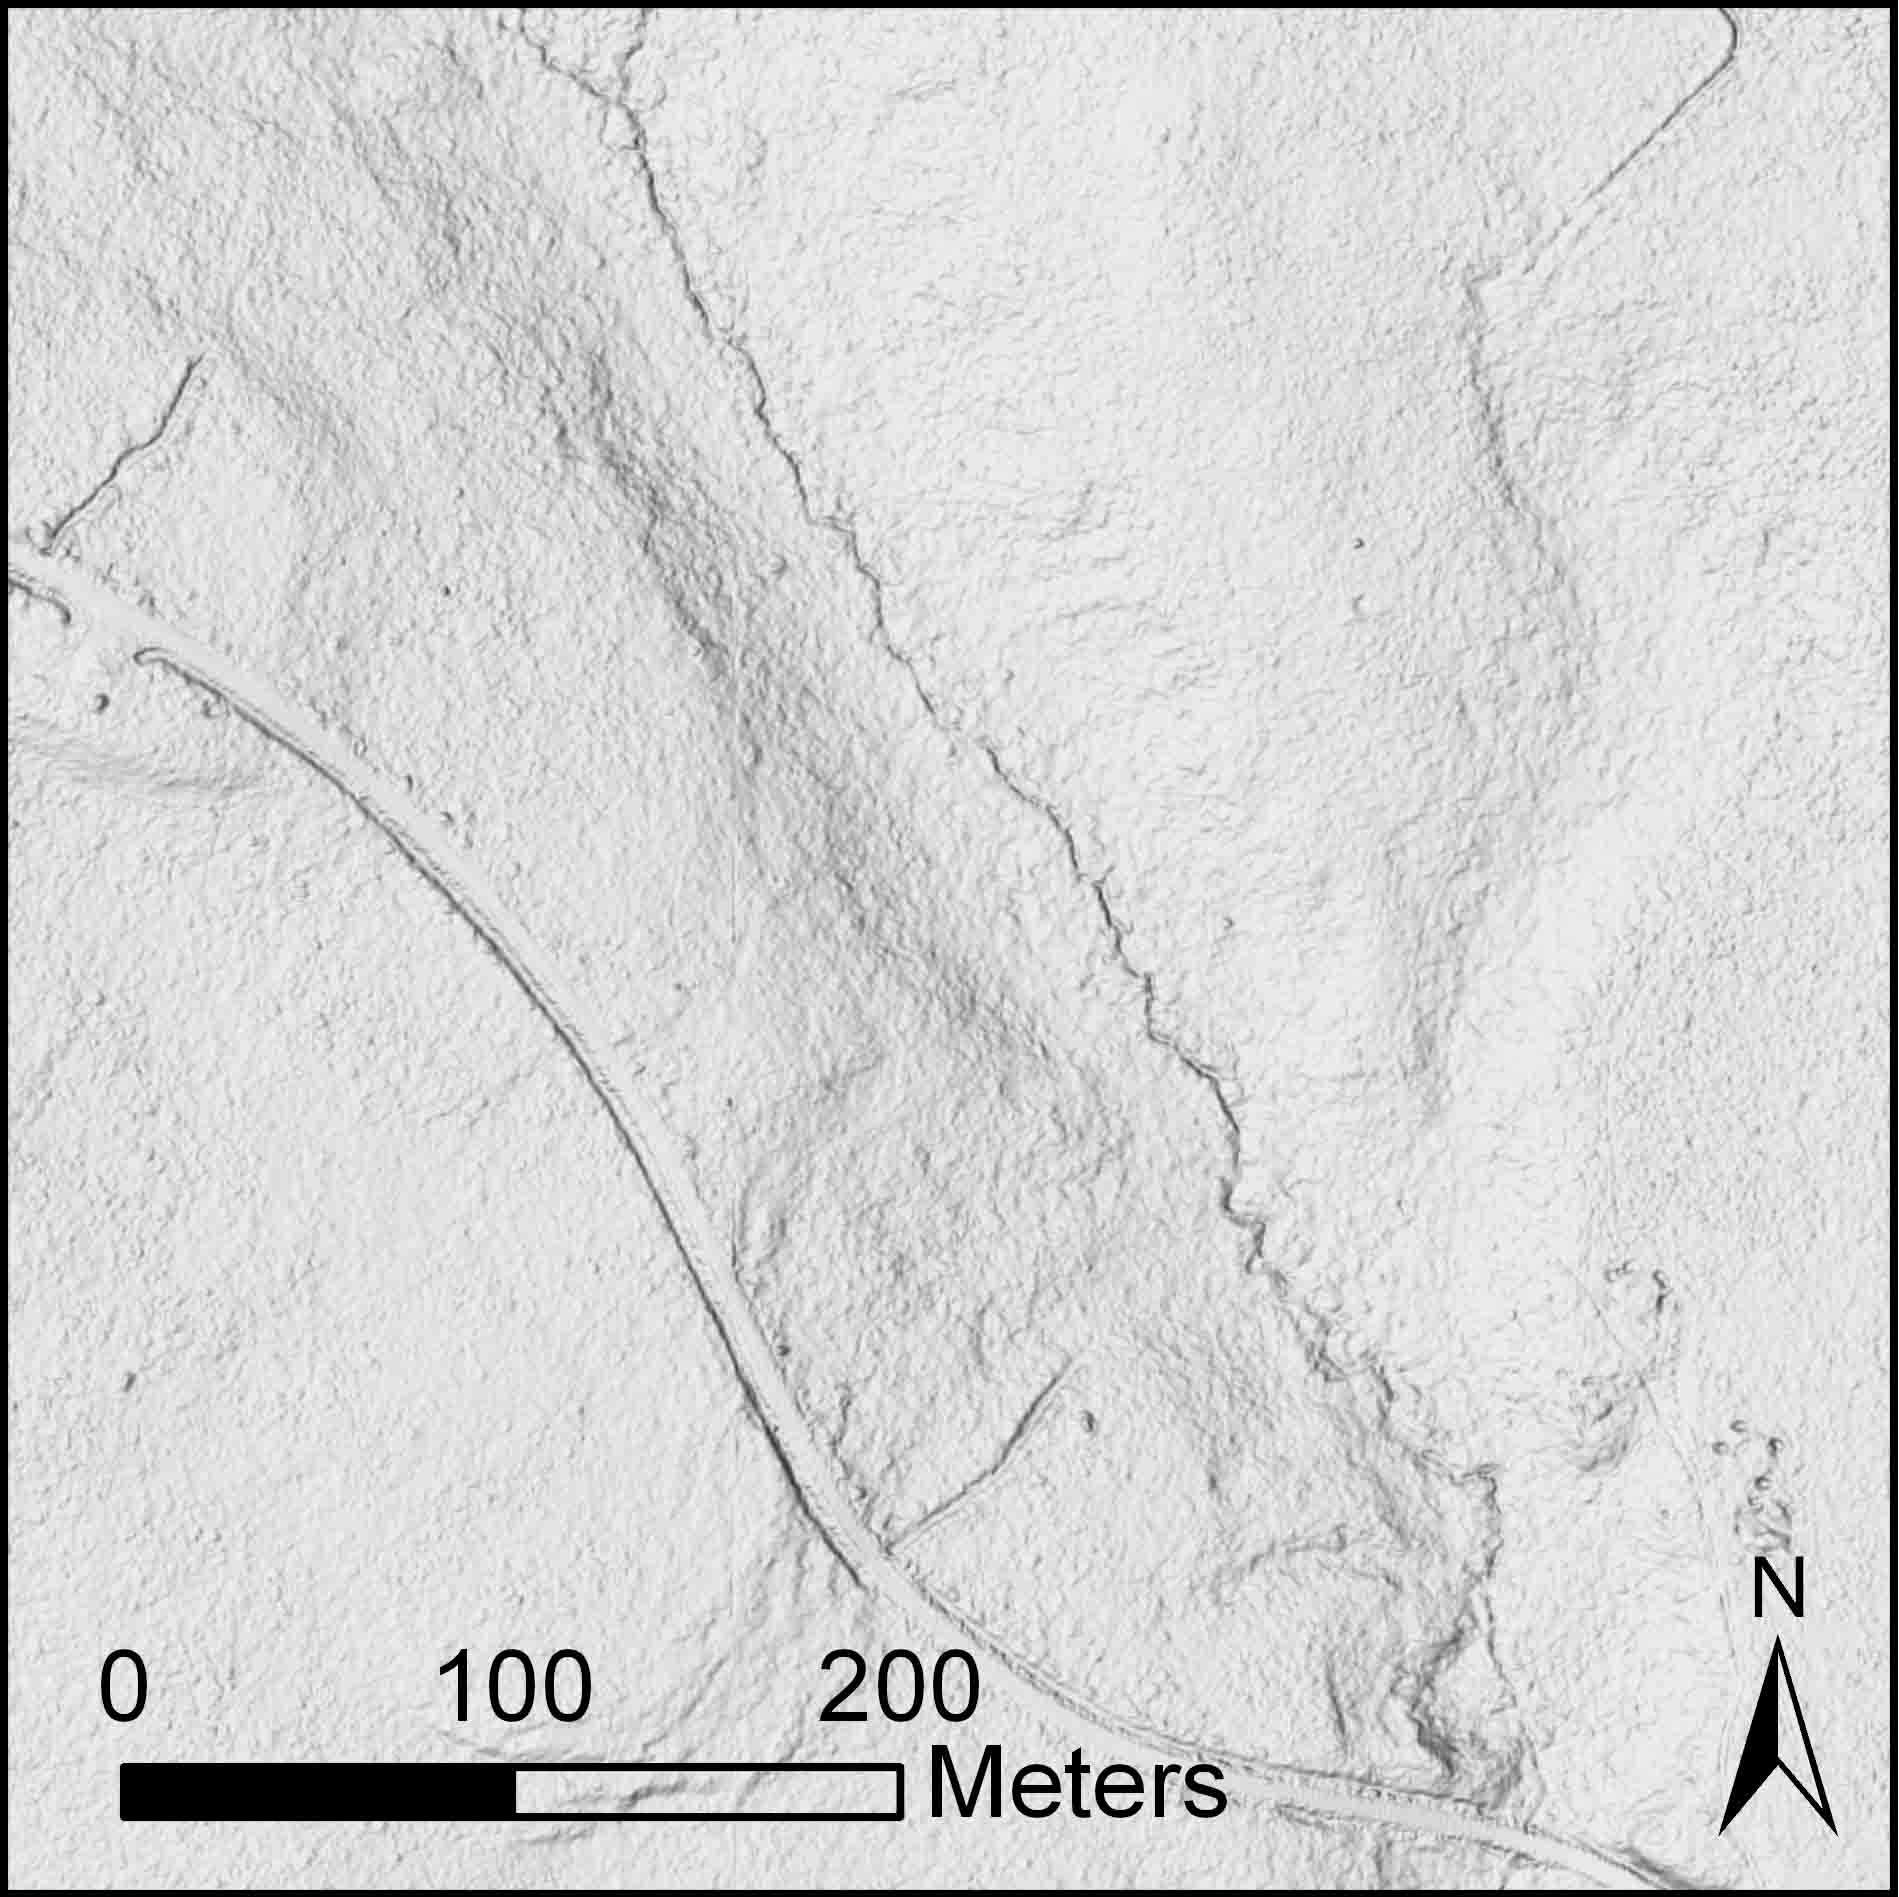
\includegraphics{./images/results_illustration_1_lo.jpg}}}\hspace{5pt}
    \subfigure[]{
        \resizebox*{4cm}{!}{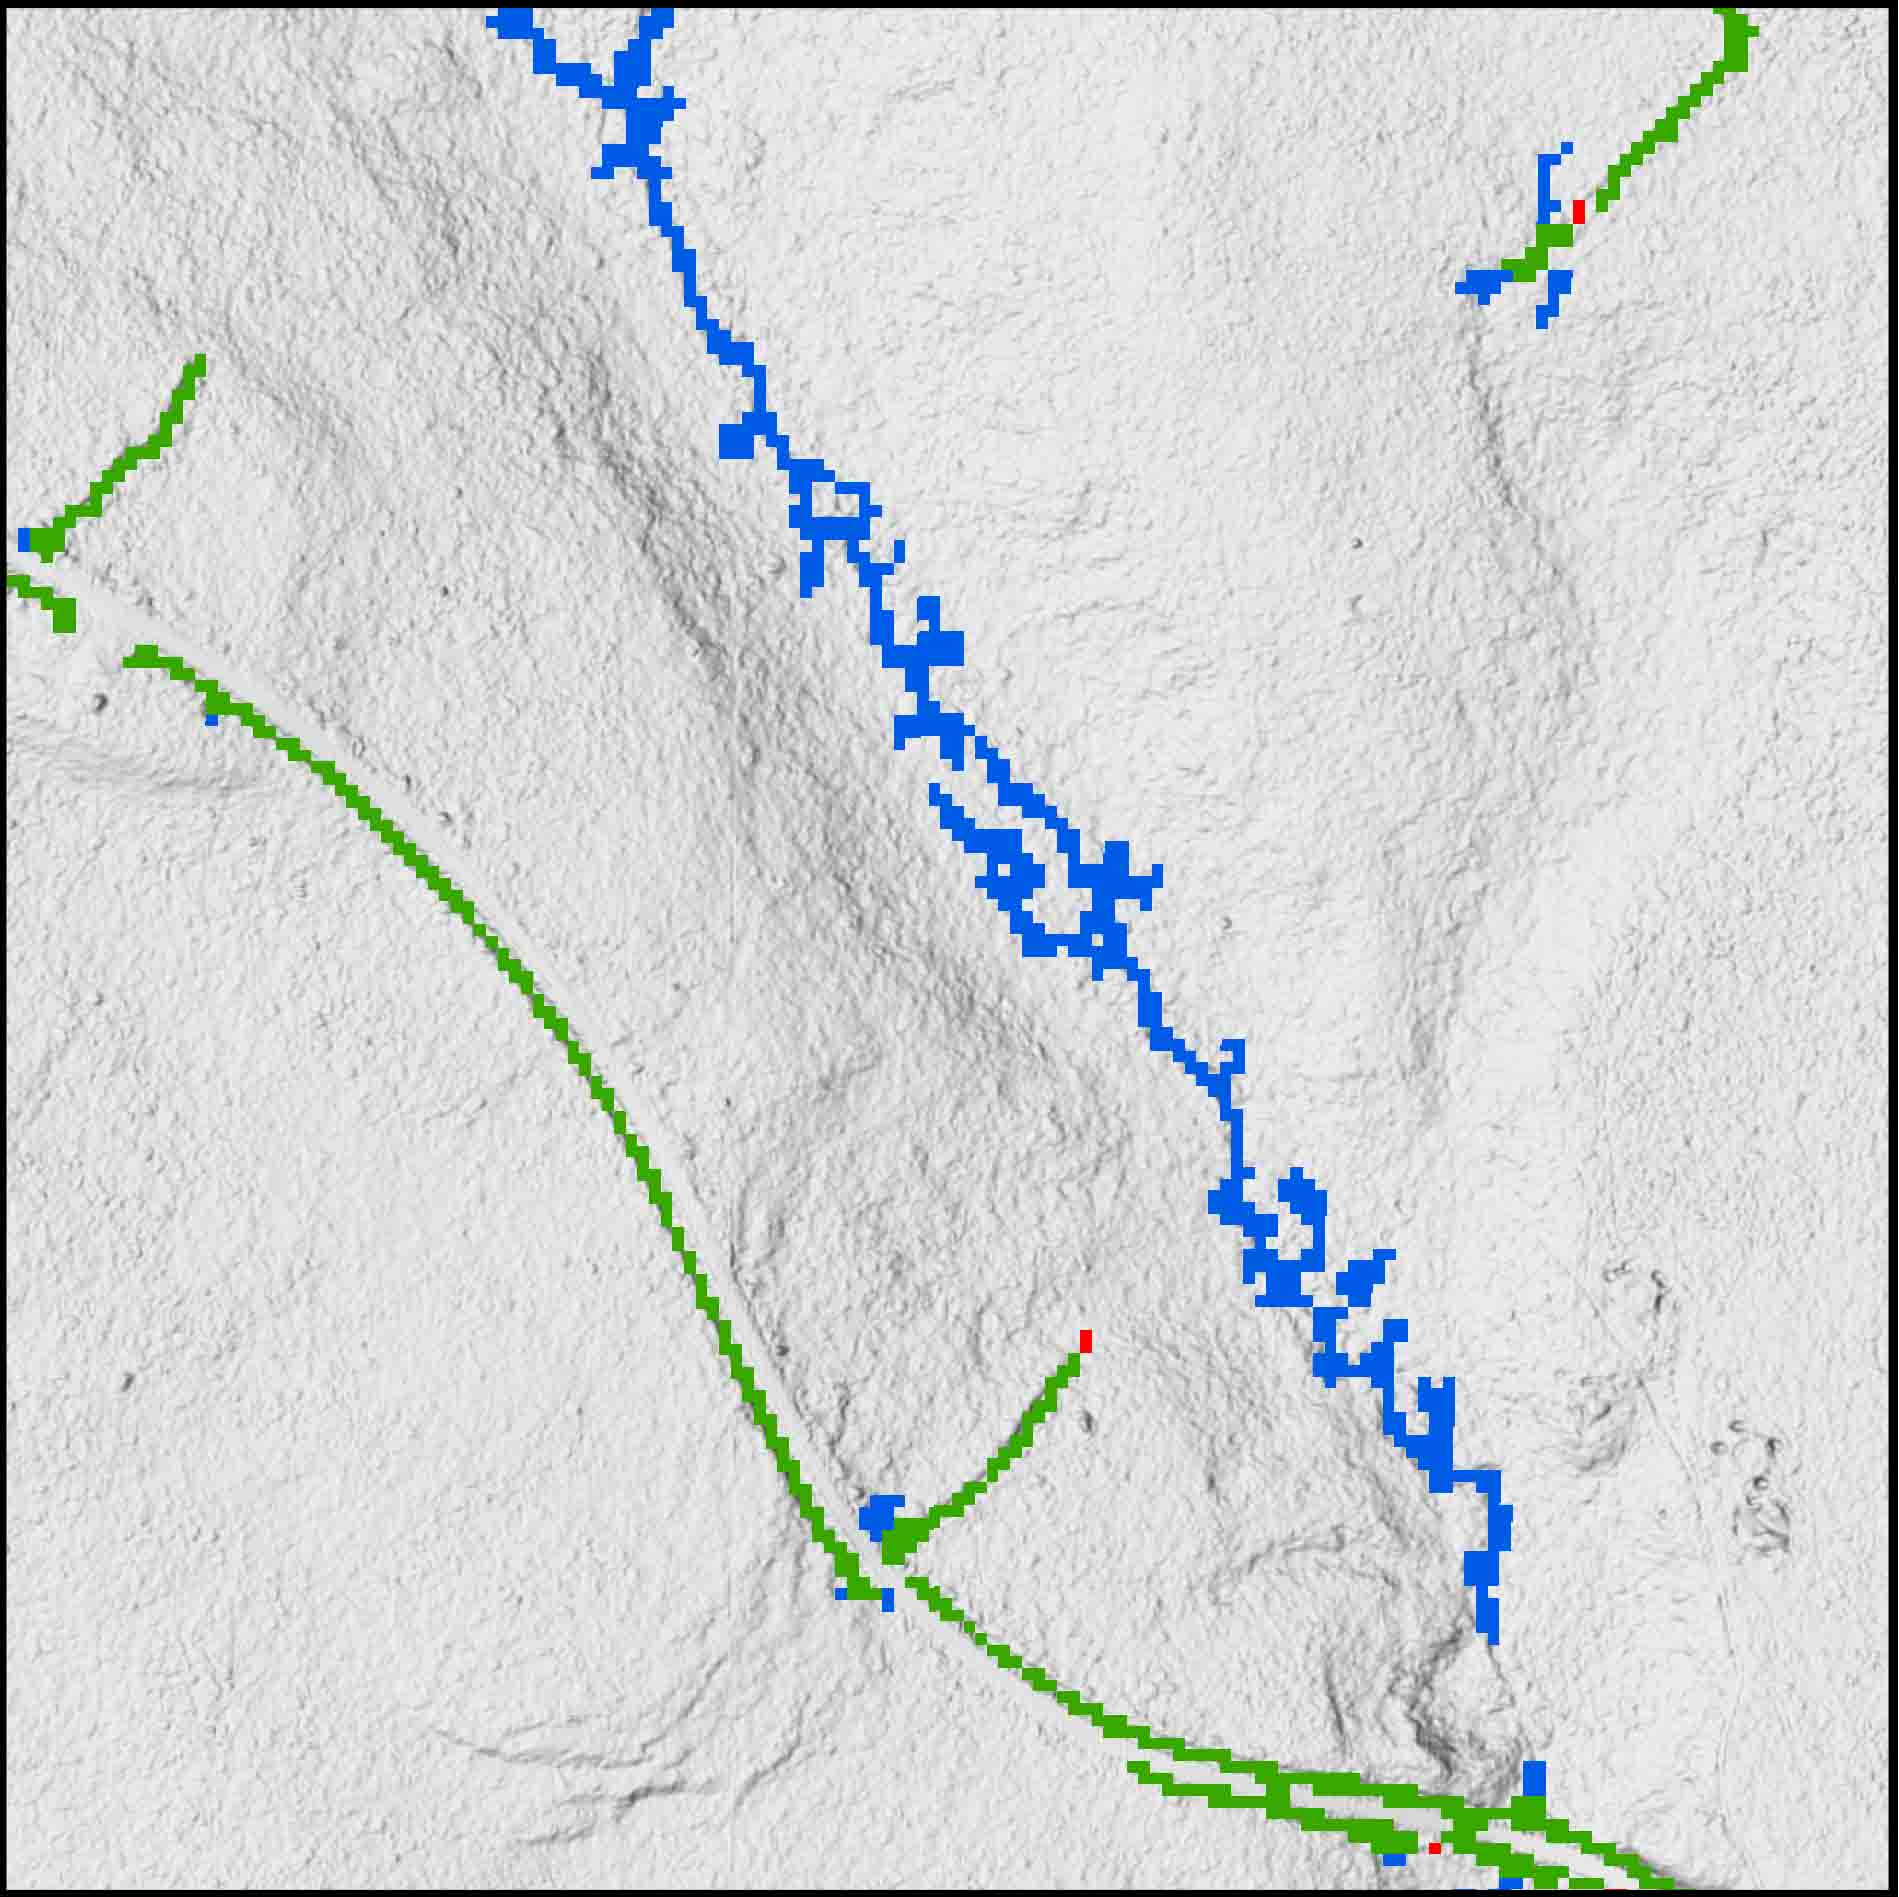
\includegraphics{./images/results_illustration_2_lo.jpg}}}
    \newline \subfigure[]{
        \resizebox*{4cm}{!}{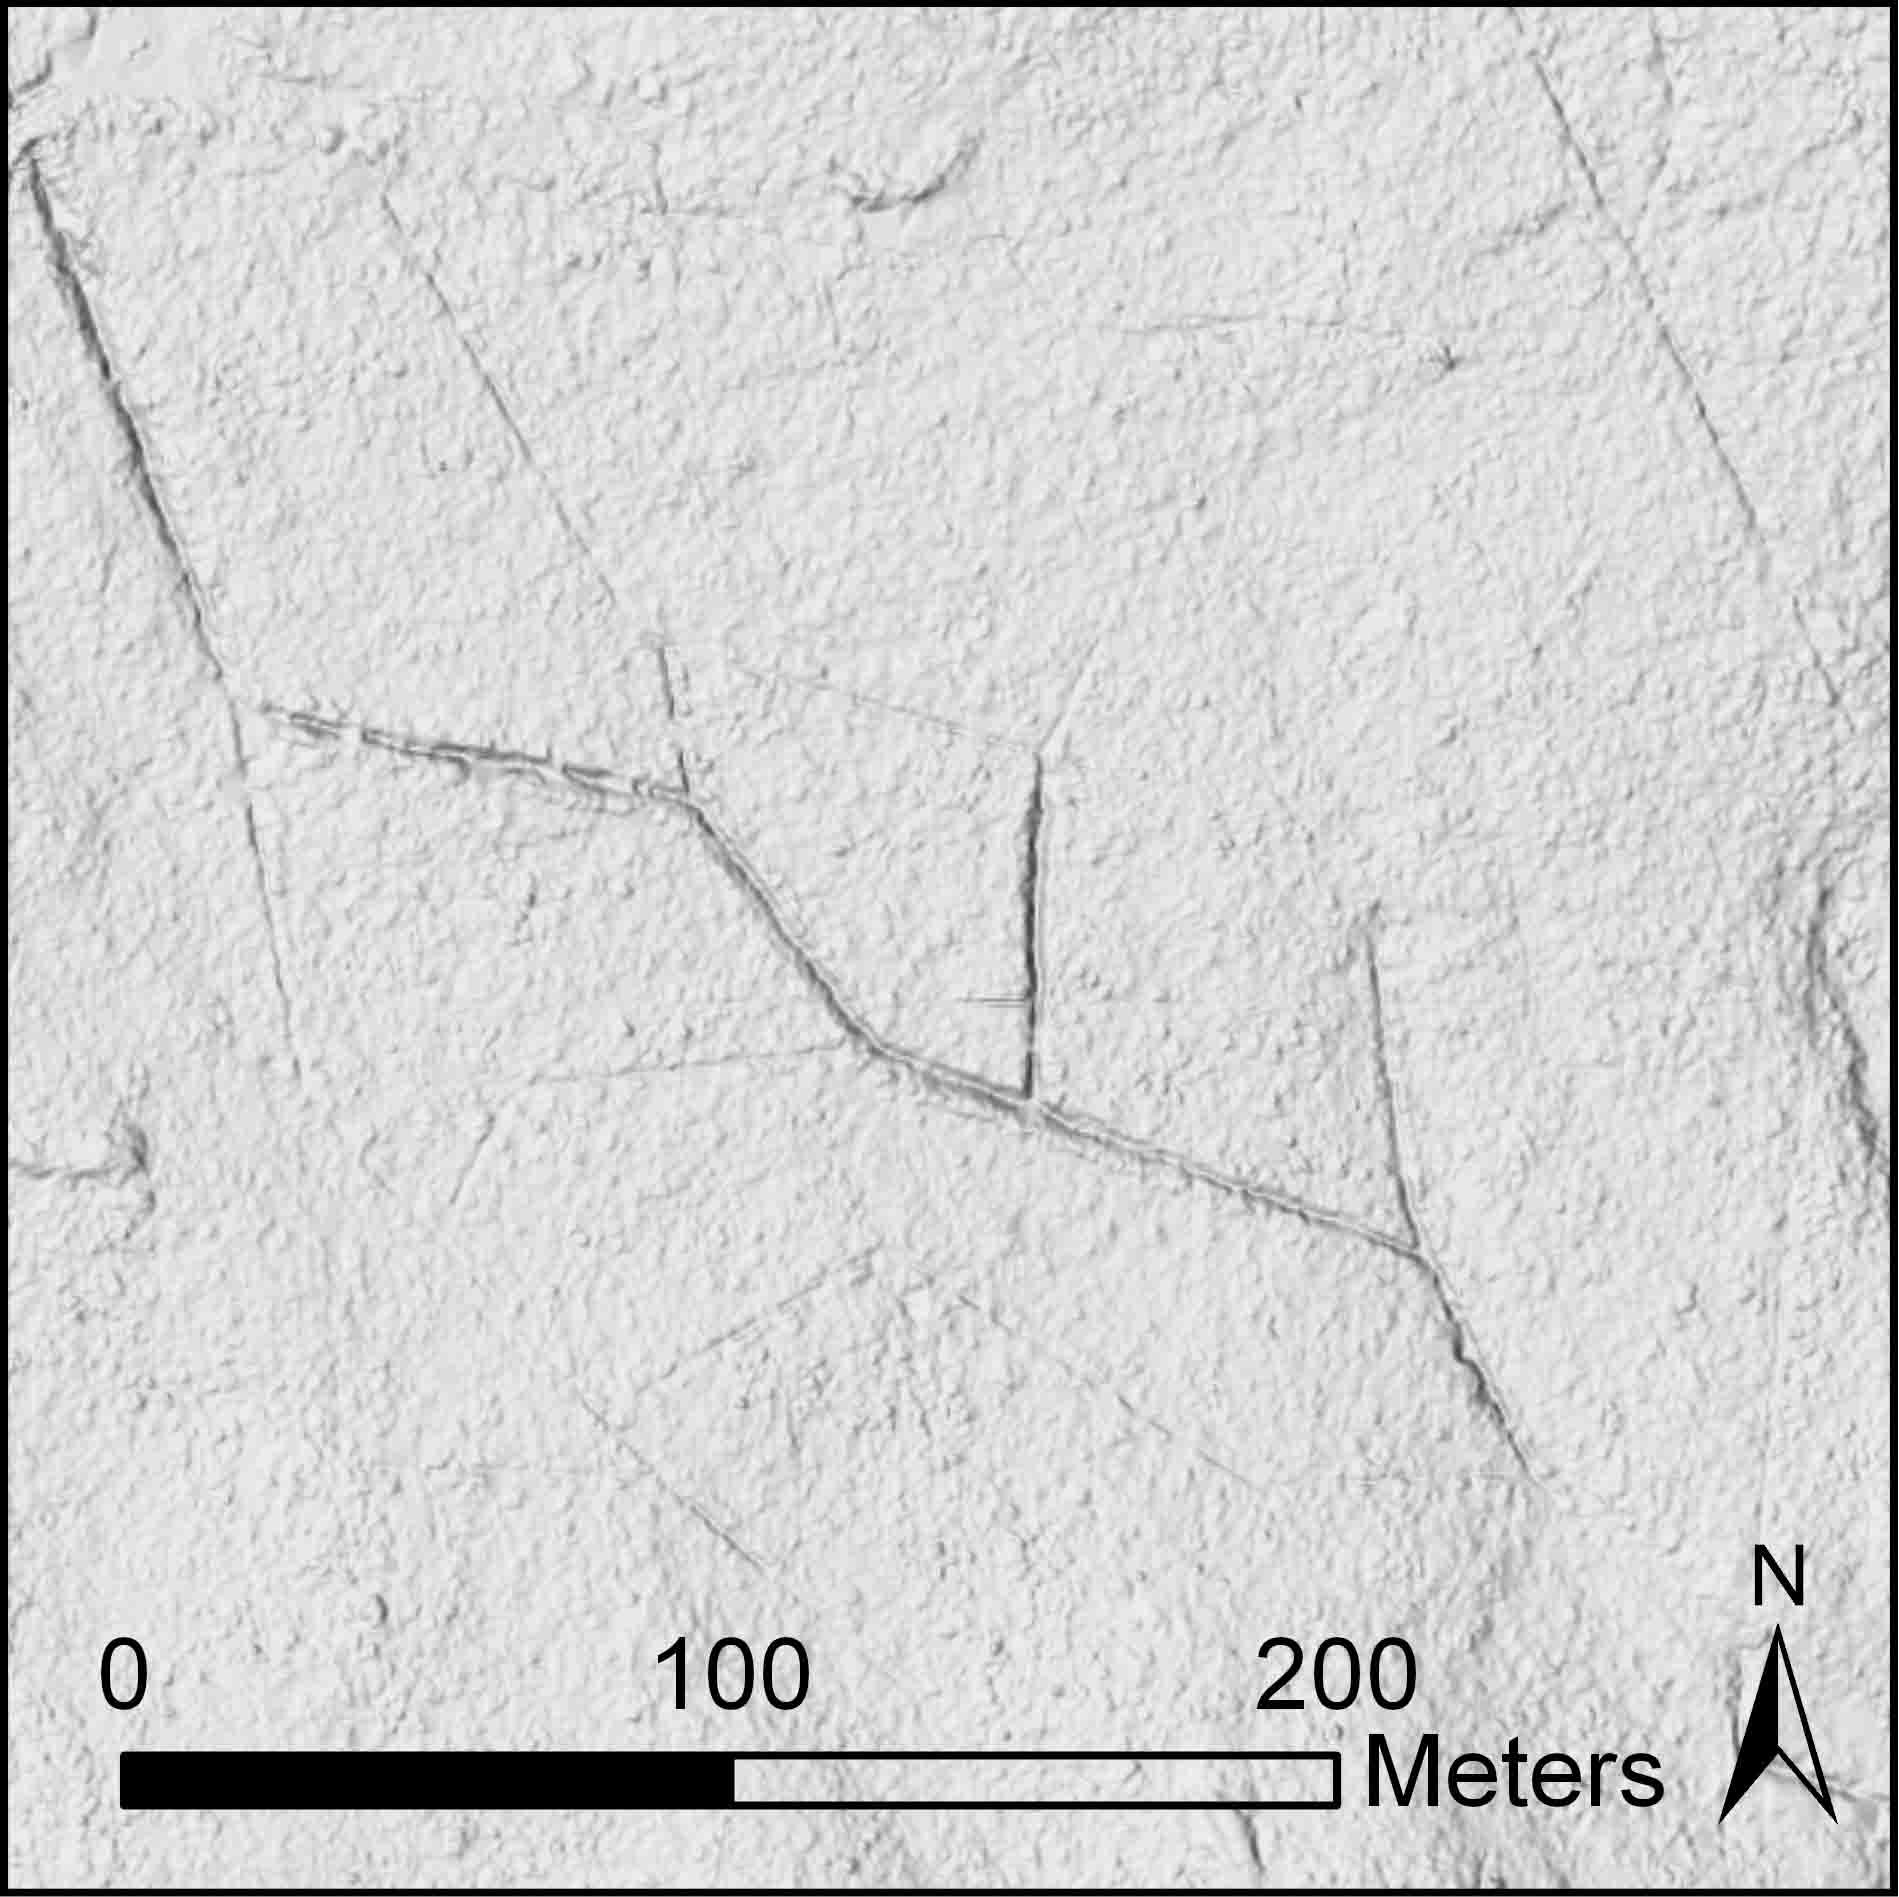
\includegraphics{./images/results_illustration_3_lo.jpg}}}\hspace{5pt}
    \subfigure[]{
        \resizebox*{4cm}{!}{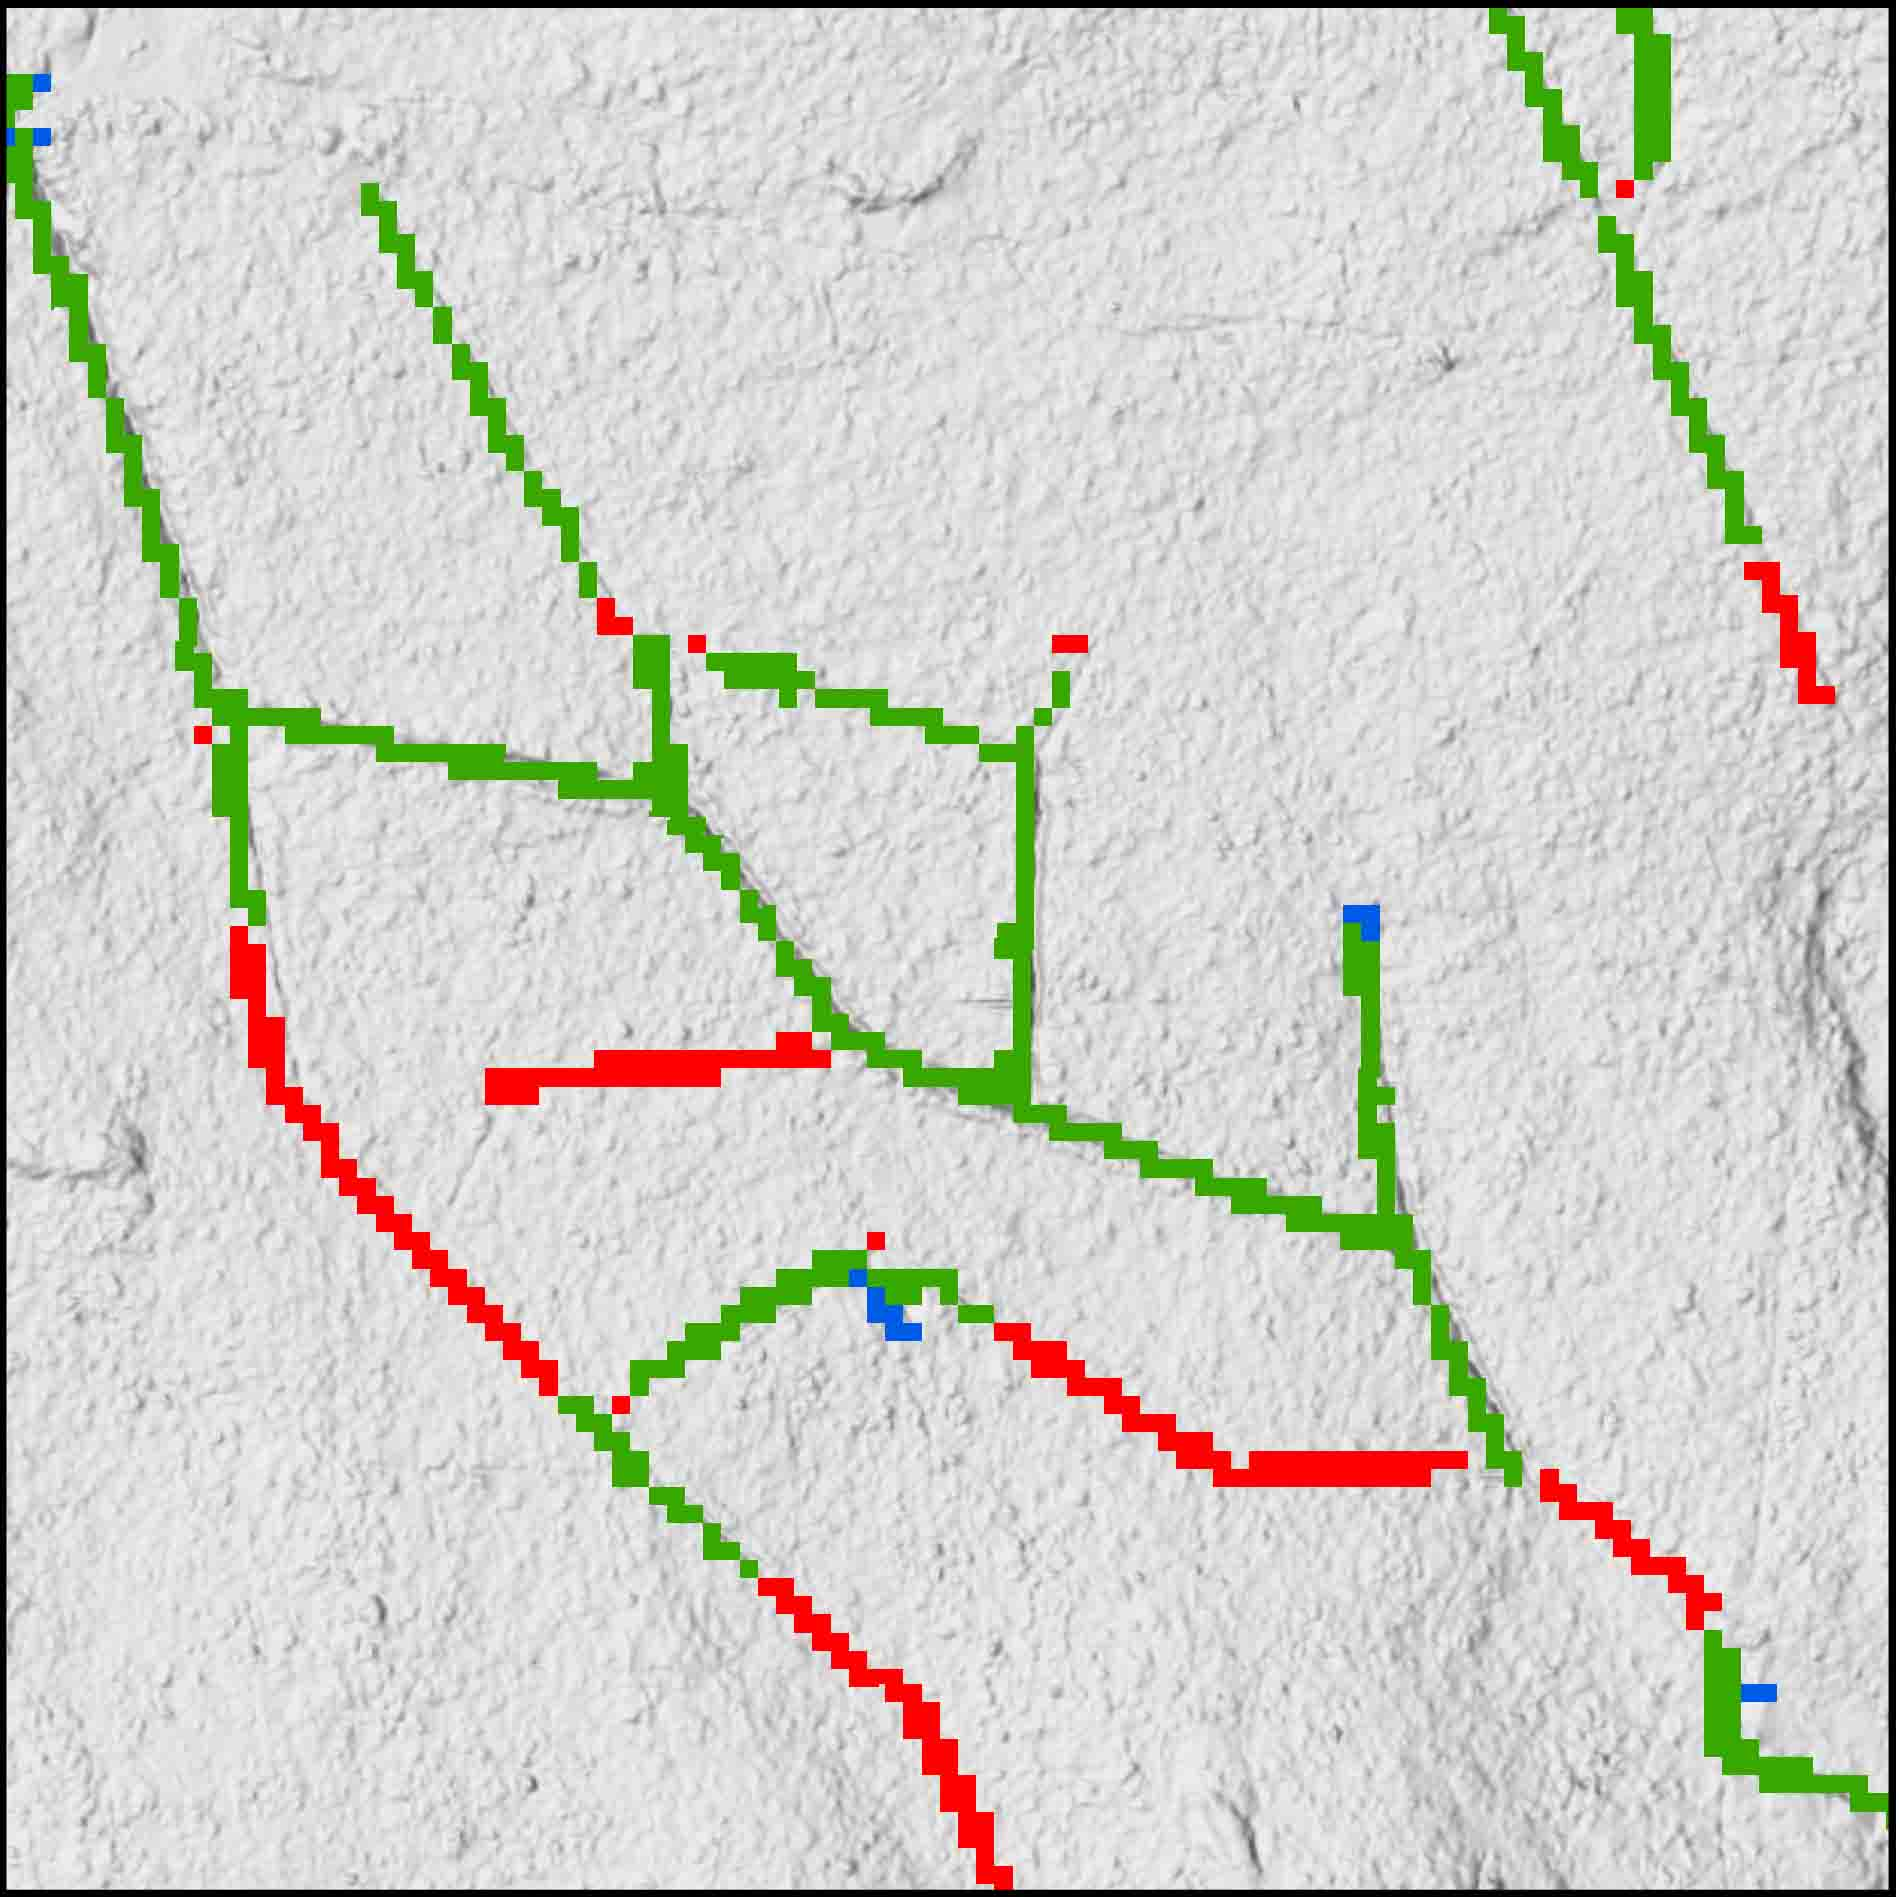
\includegraphics{./images/results_illustration_4_lo.jpg}}}
    \newline \subfigure[]{
        \resizebox*{4cm}{!}{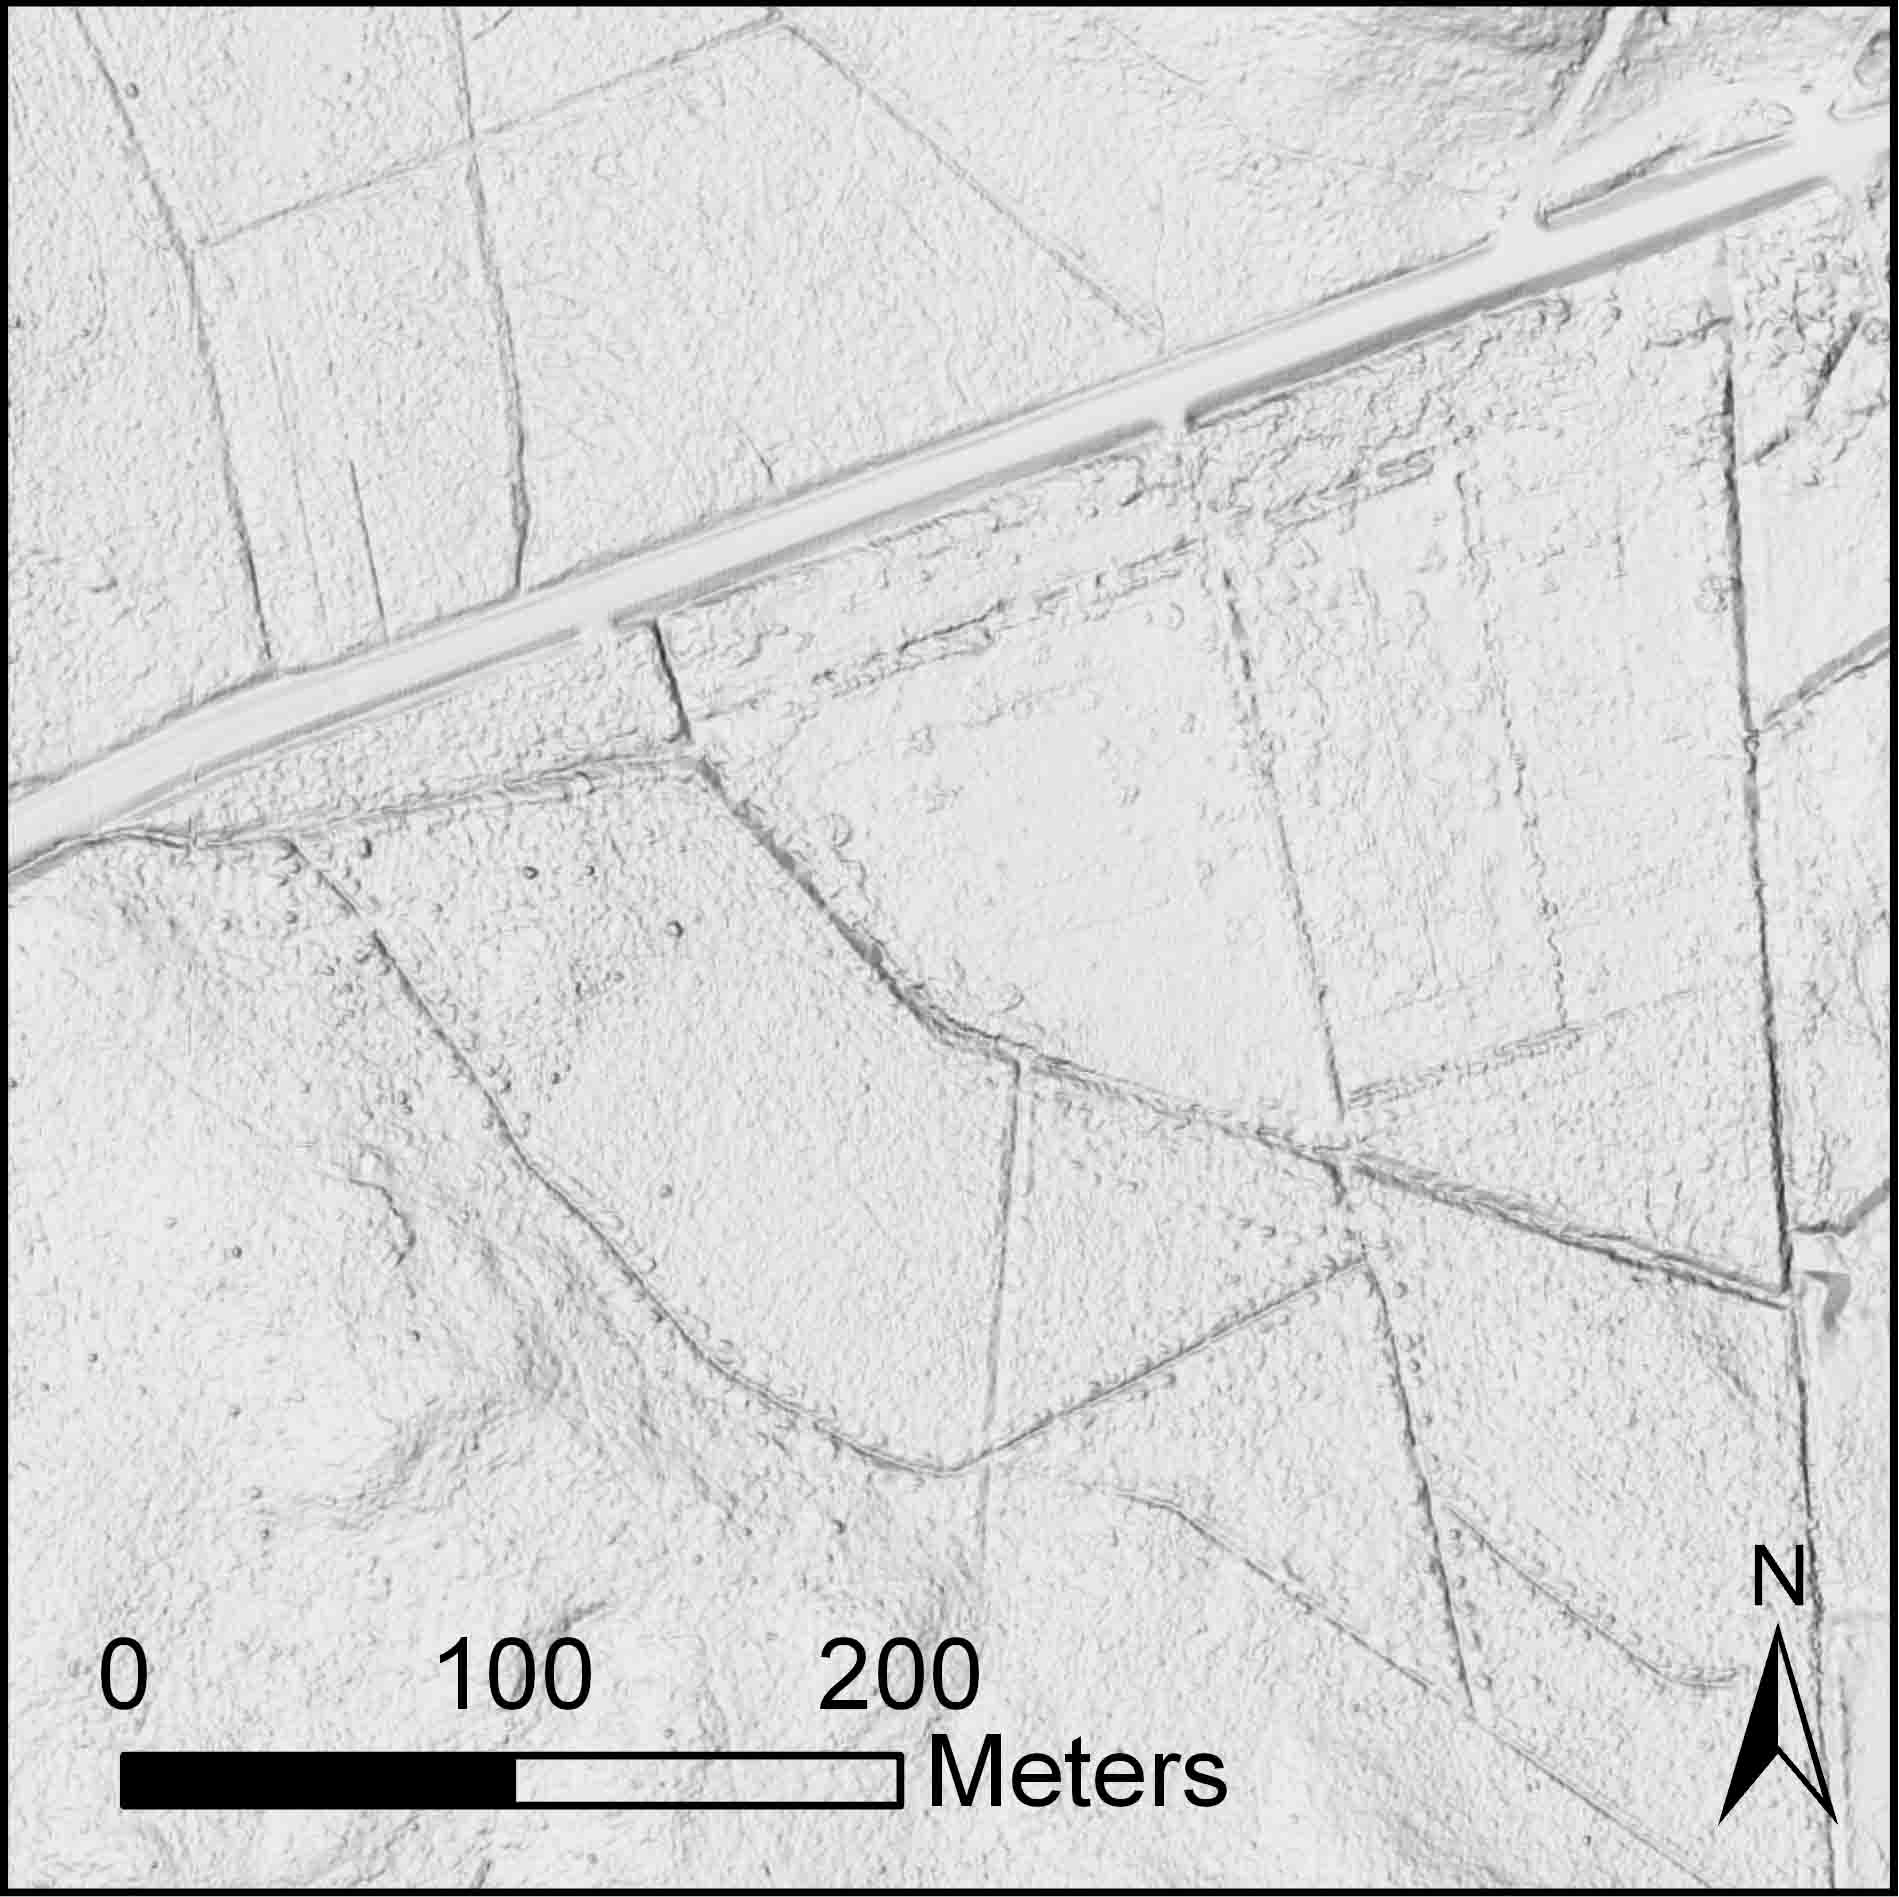
\includegraphics{./images/results_illustration_5_lo.jpg}}}\hspace{5pt}
    \subfigure[]{
        \resizebox*{4cm}{!}{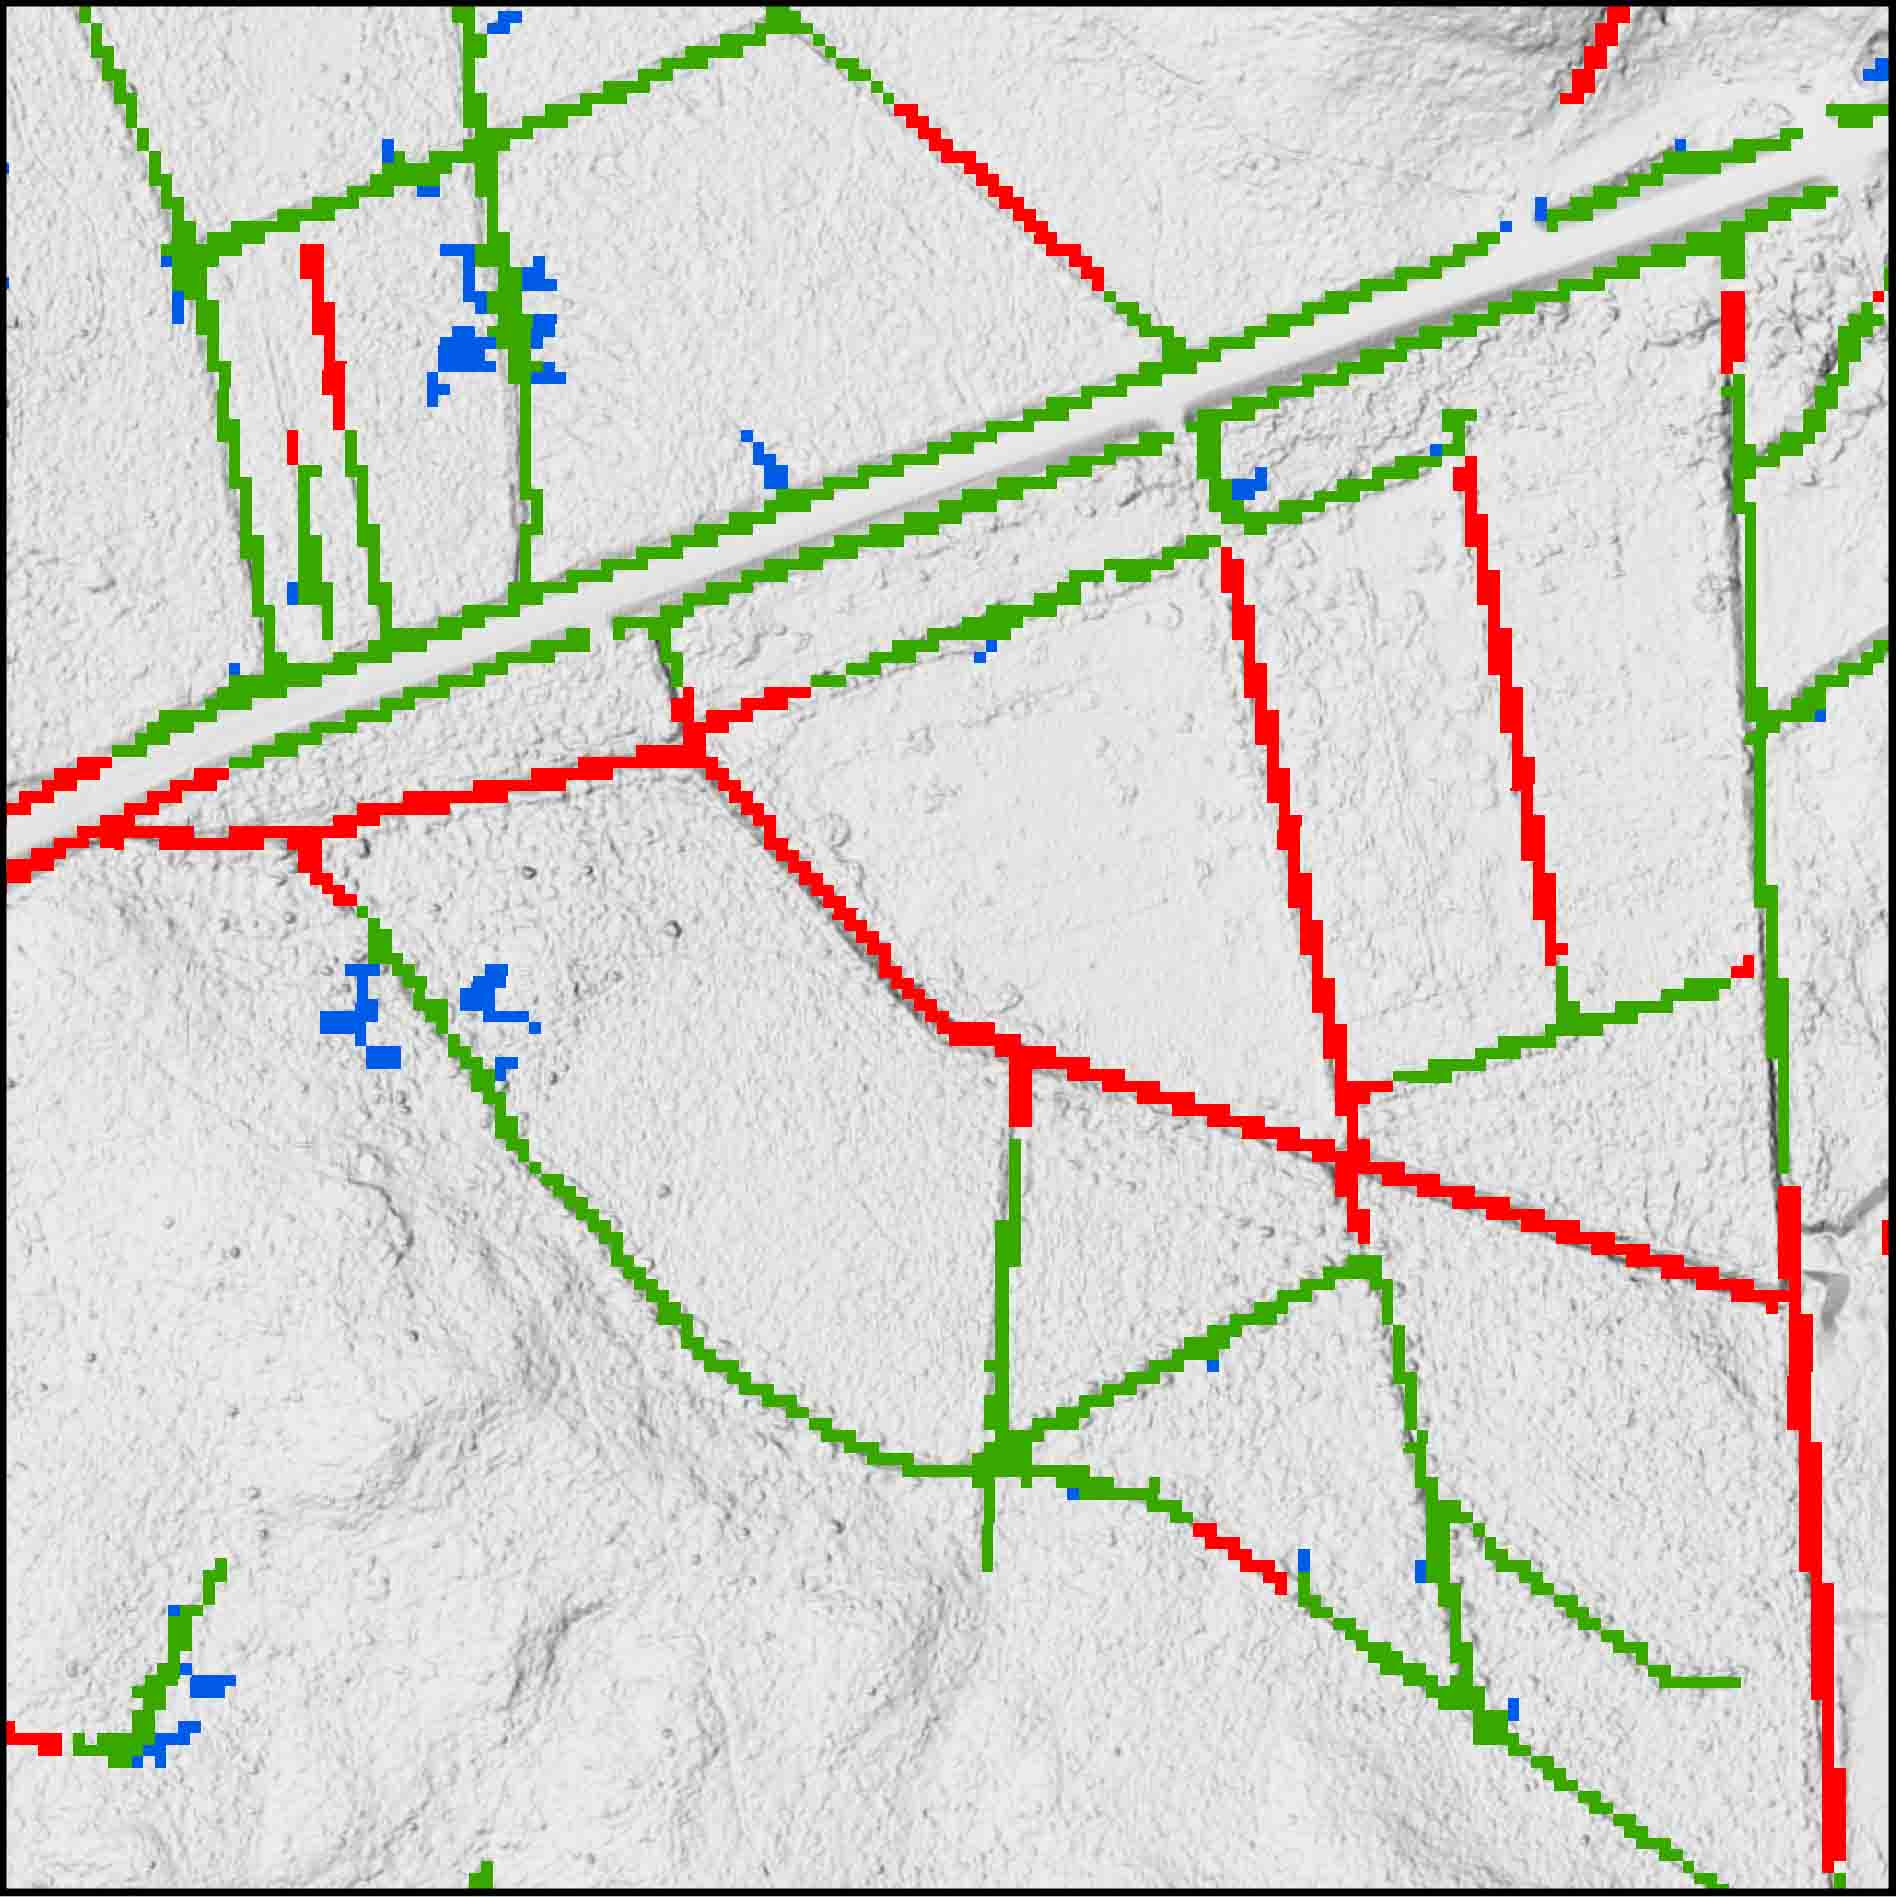
\includegraphics{./images/results_illustration_6_lo.jpg}}}
    \newline
    \caption{\textbf{Visual analysis of ditch detector.} The left panel shows the hillshade for a number of subsections, and the right panel shows the hillshade with the extracted ditches superimposed on top. Green marks correctly classified ditches (true positives), red marks missed ditches (false negatives), blue marks incorrectly classified ditches (false positives), and transparent areas mark correctly classified non-ditches (true negatives). \textbf{a} and \textbf{b} illustrate that the most common false positives were natural stream channels being classified as ditches. \textbf{c} and \textbf{d} illustrate that very shallow ditches that were barely visible in the DEM were not captured with our ditch detector. \textbf{e} and \textbf{f} illustrate that some of the deepest and more prominent ditches were also missed. This occurred as a result of attempting to get rid of more false positives in the form of streams by using the features explained in \ref{impoundmentstreamremoval}.}
    \label{fig:resultsillustrations}
\end{figure}

In \hyperref[featureimportancetable]{Table} \ref{featureimportancetable}, the top 20 (out of 40) features from the Random Forests model are presented with their Gini importances \citep{gini}. Features derived from the \hyperref[hpmf]{HPMF} and \hyperref[impoundment]{Impoundment} terrain indices contributed the most to a successful prediction. The features that used statistical aggregation methods on the neighbouring area around pixels, as well as the stream removal and Gabor filter features also performed well.

\begin{table} [!htb]
\centering
    {\begin{tabular}{r|ll}
      Pos & Variable\textsuperscript{a} & Importance (\%) \\
      \hline
      1.  & Impoundment mean 3                                  & 7.33\\
      2.  & HPMF mean 4                                         & 6.23\\
      3.  & Impoundment mean 4                                  & 5.57\\
      4.  & Impoundment mean 2                                  & 5.41\\
      5.  & HPMF mean 3                                         & 4.33\\
      6.  & Impoundment median 4                                & 3.84\\
      7.  & HPMF Gabor - streams removed                        & 3.54\\
      8.  & HPMF median 4                                       & 3.40\\
      9.  & Impoundment median 2                                & 3.01\\
      10. & Sky View Factor Gabor - streams removed             & 2.84\\
      11. & HPMF mean 6                                         & 2.73\\
      12. & Impoundment median 6                                & 2.69\\
      13. & Impoundment standard deviation 4                    & 2.52\\
      14. & Sky View Factor Gabor                               & 2.44\\
      15. & Impoundment ditch amplification                     & 2.43\\
      16. & Impoundment mean 6                                  & 2.27\\
      17. & Impoundment ditch amplification - streams removed   & 2.24\\
      18. & HPMF min 2                                          & 2.23\\
      19. & Slope standard deviation 6                          & 2.01\\
      20. & Sky View Factor non-ditch amplification             & 1.88\\
      \hline
    \end{tabular}}
    \caption{\textbf{Feature importances.} The top 20 features (out of 40) by Gini importance. \newline \textsuperscript{a} The number next to some of the variables indicates the circular radius used to select what neighbouring pixels to use in the statistical aggregation method. The radii represents pixels with a 0.5 m resolution.}
    \label{featureimportancetable}
\end{table}

\section{Discussion}

Our study has shown that it is possible to locate ditches automatically in high-resolution DEMs ($0.5  * 0.5 $ metres, in our case), and that more of the ditches can be detected if several terrain indices (\hyperref[predictionperformance]{Table} \ref{predictionperformance}) are combined through machine learning than if indices are used separately (\hyperref[recreatedpredictionperformance]{Table} \ref{recreatedpredictionperformance}). The ditch detection performance varied depending on the type of ditches, this is illustrated in \hyperref[fig:ditchpictures]{Figure} \ref{fig:ditchpictures}. For example, the retrieval rate was slightly higher for the road ditches compared to forest or agricultural ditches. This is likely due to the fact that  road ditches are found in open areas alongside roads, and also,   they are generally well maintained for optimum functioning (\hyperref[fig:ditchpictures]{Figure} \ref{fig:ditchpictures} \hyperref[fig:ditchpictures]{a}). However, most of the ditches in Krycklan today are found below the canopy (e.g. \hyperref[fig:ditchpictures]{Figure} \ref{fig:ditchpictures} \hyperref[fig:ditchpictures]{c}), and the majority have not been maintained, causing difficulties in detecting them as some have grown back in with peat, grasses, or shrubs (\hyperref[fig:resultstreesbushes]{Figure} \ref{fig:resultstreesbushes} \hyperref[fig:resultstreesbushes]{b}). This, in combination with the surrounding peat having subsided \citep{heikurainen}, have rendered them almost impossible to detect in the DEM today (\hyperref[fig:ditchpictures]{Figure} \ref{fig:ditchpictures} \hyperref[fig:ditchpictures]{d}). Despite these issues we had a recall rate of 70.28\%, showing that the majority of the ditches could still be retrieved automatically.


\begin{figure} [!htb]
\centering
    \subfigure[]{
        \resizebox*{6.8cm}{!}{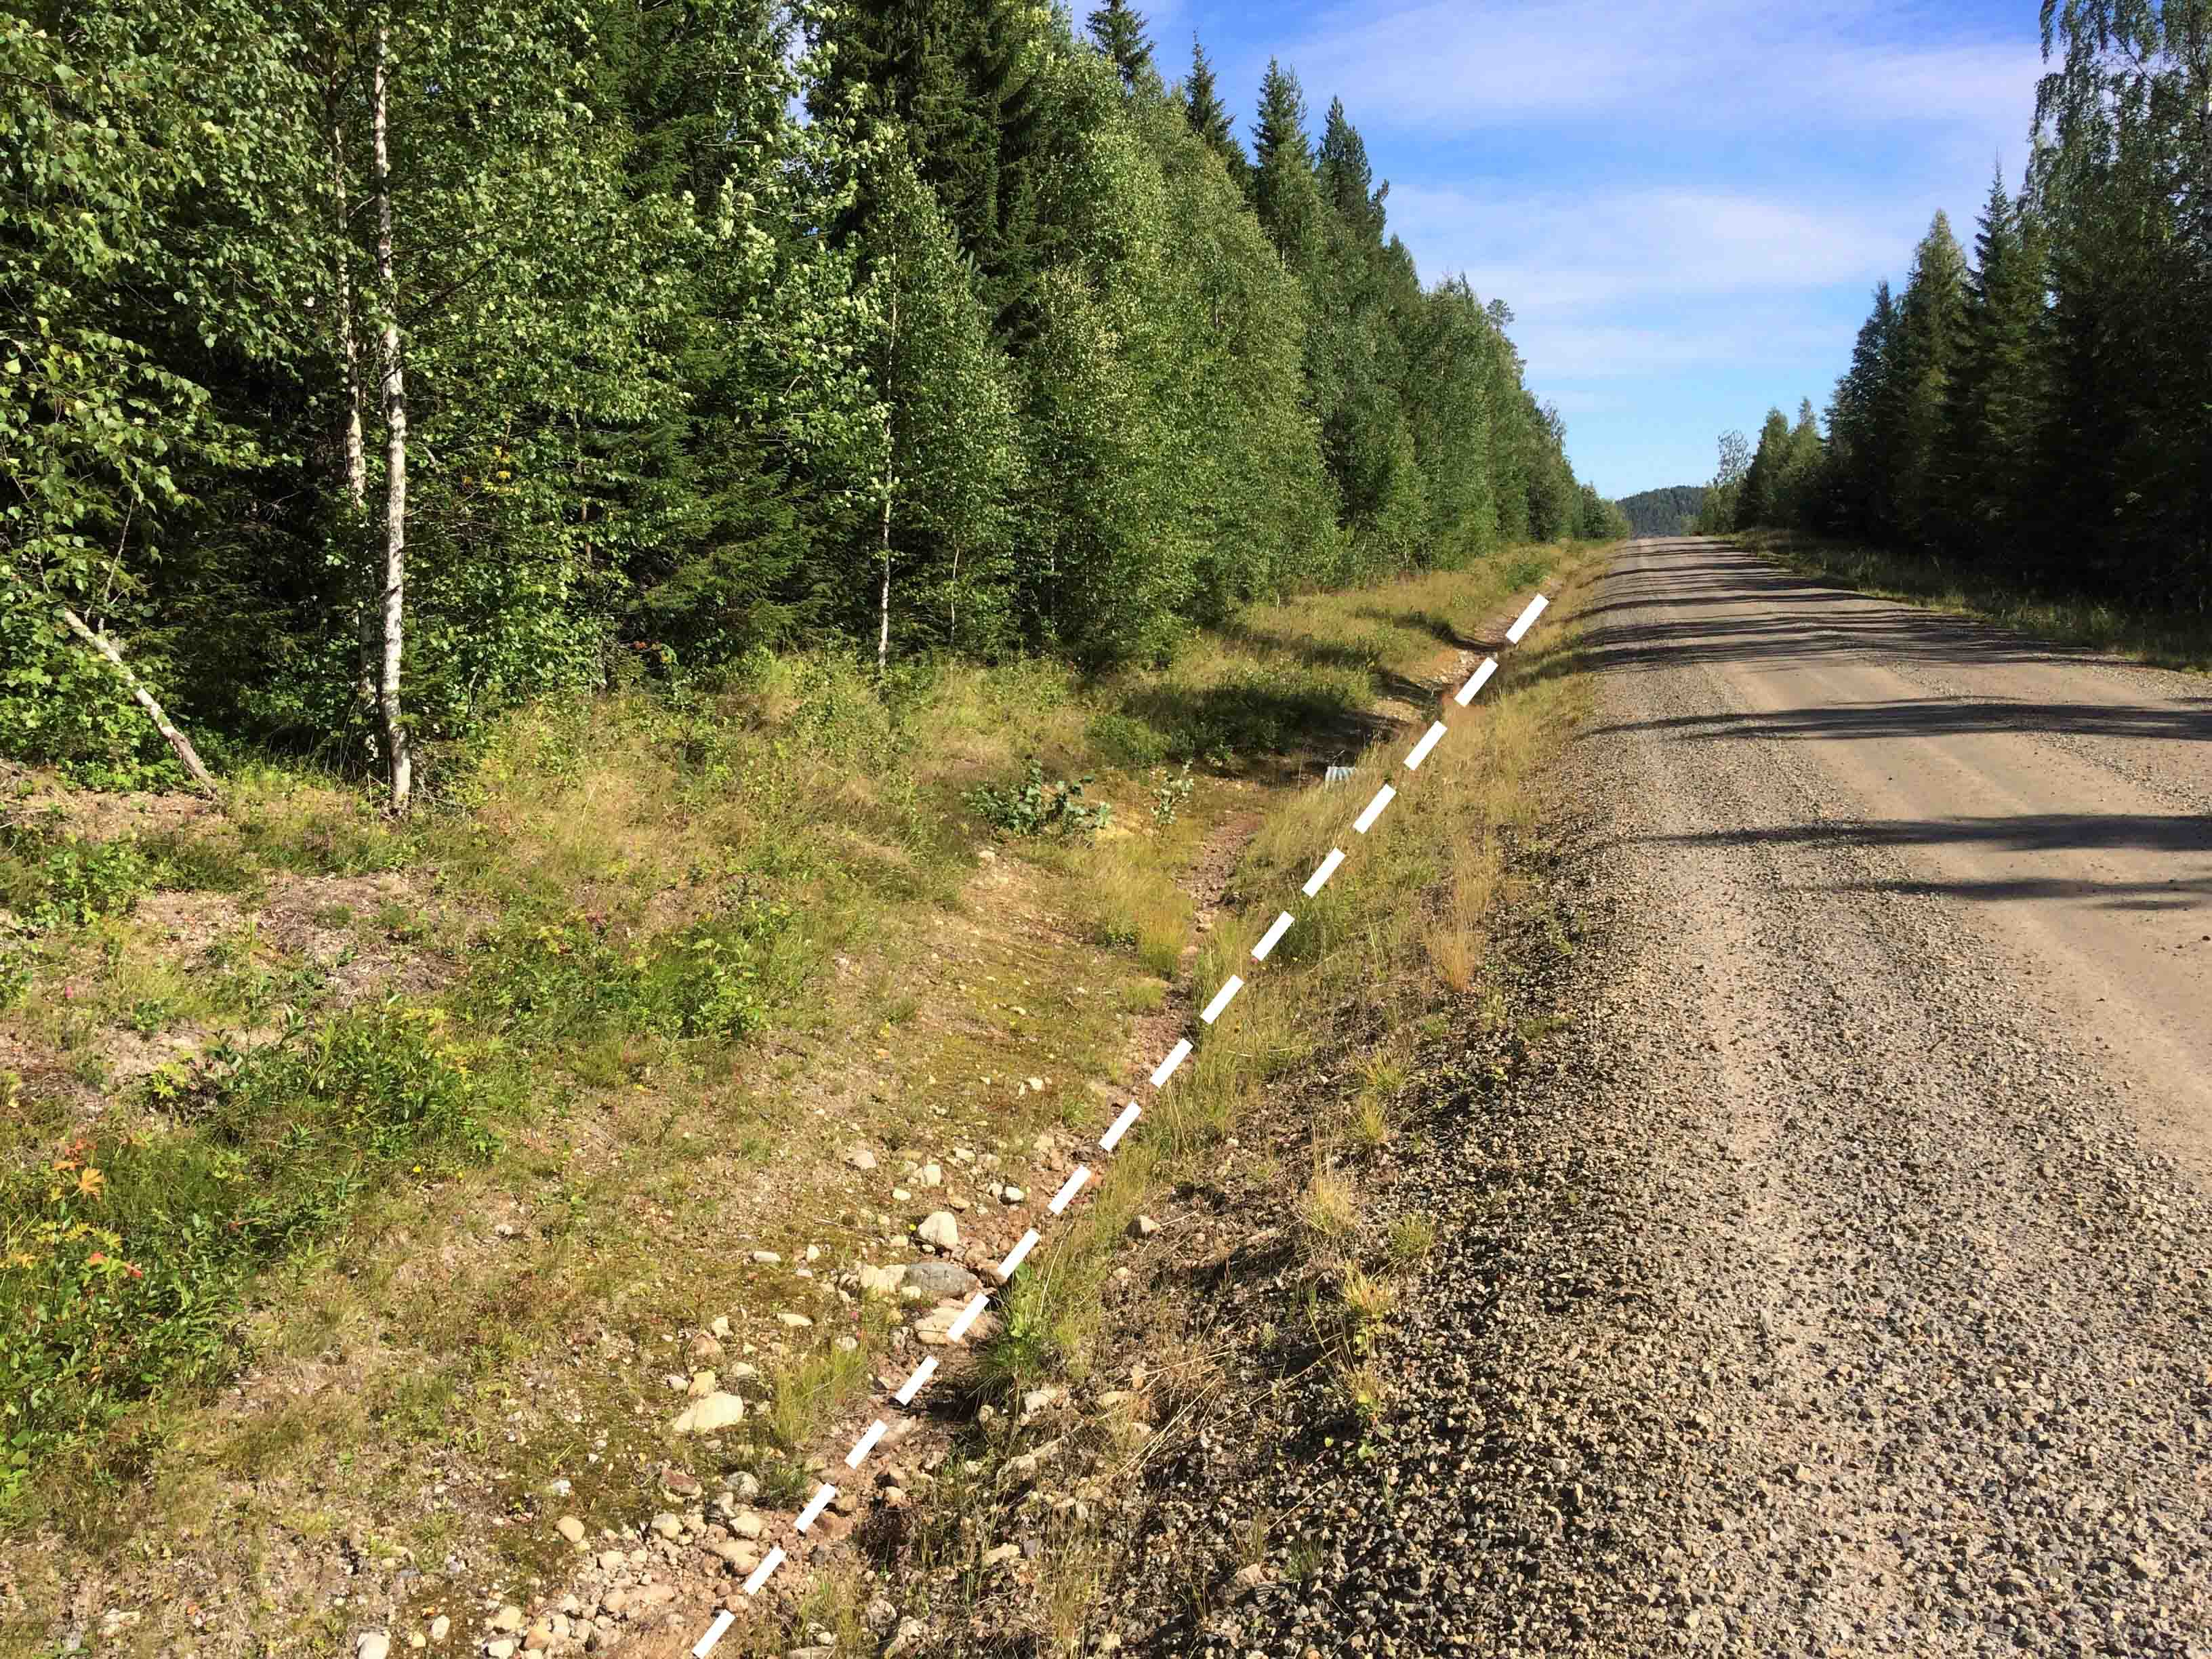
\includegraphics{./images/road_ditch_lo.jpg}}}
    \subfigure[]{
        \resizebox*{6.8cm}{!}{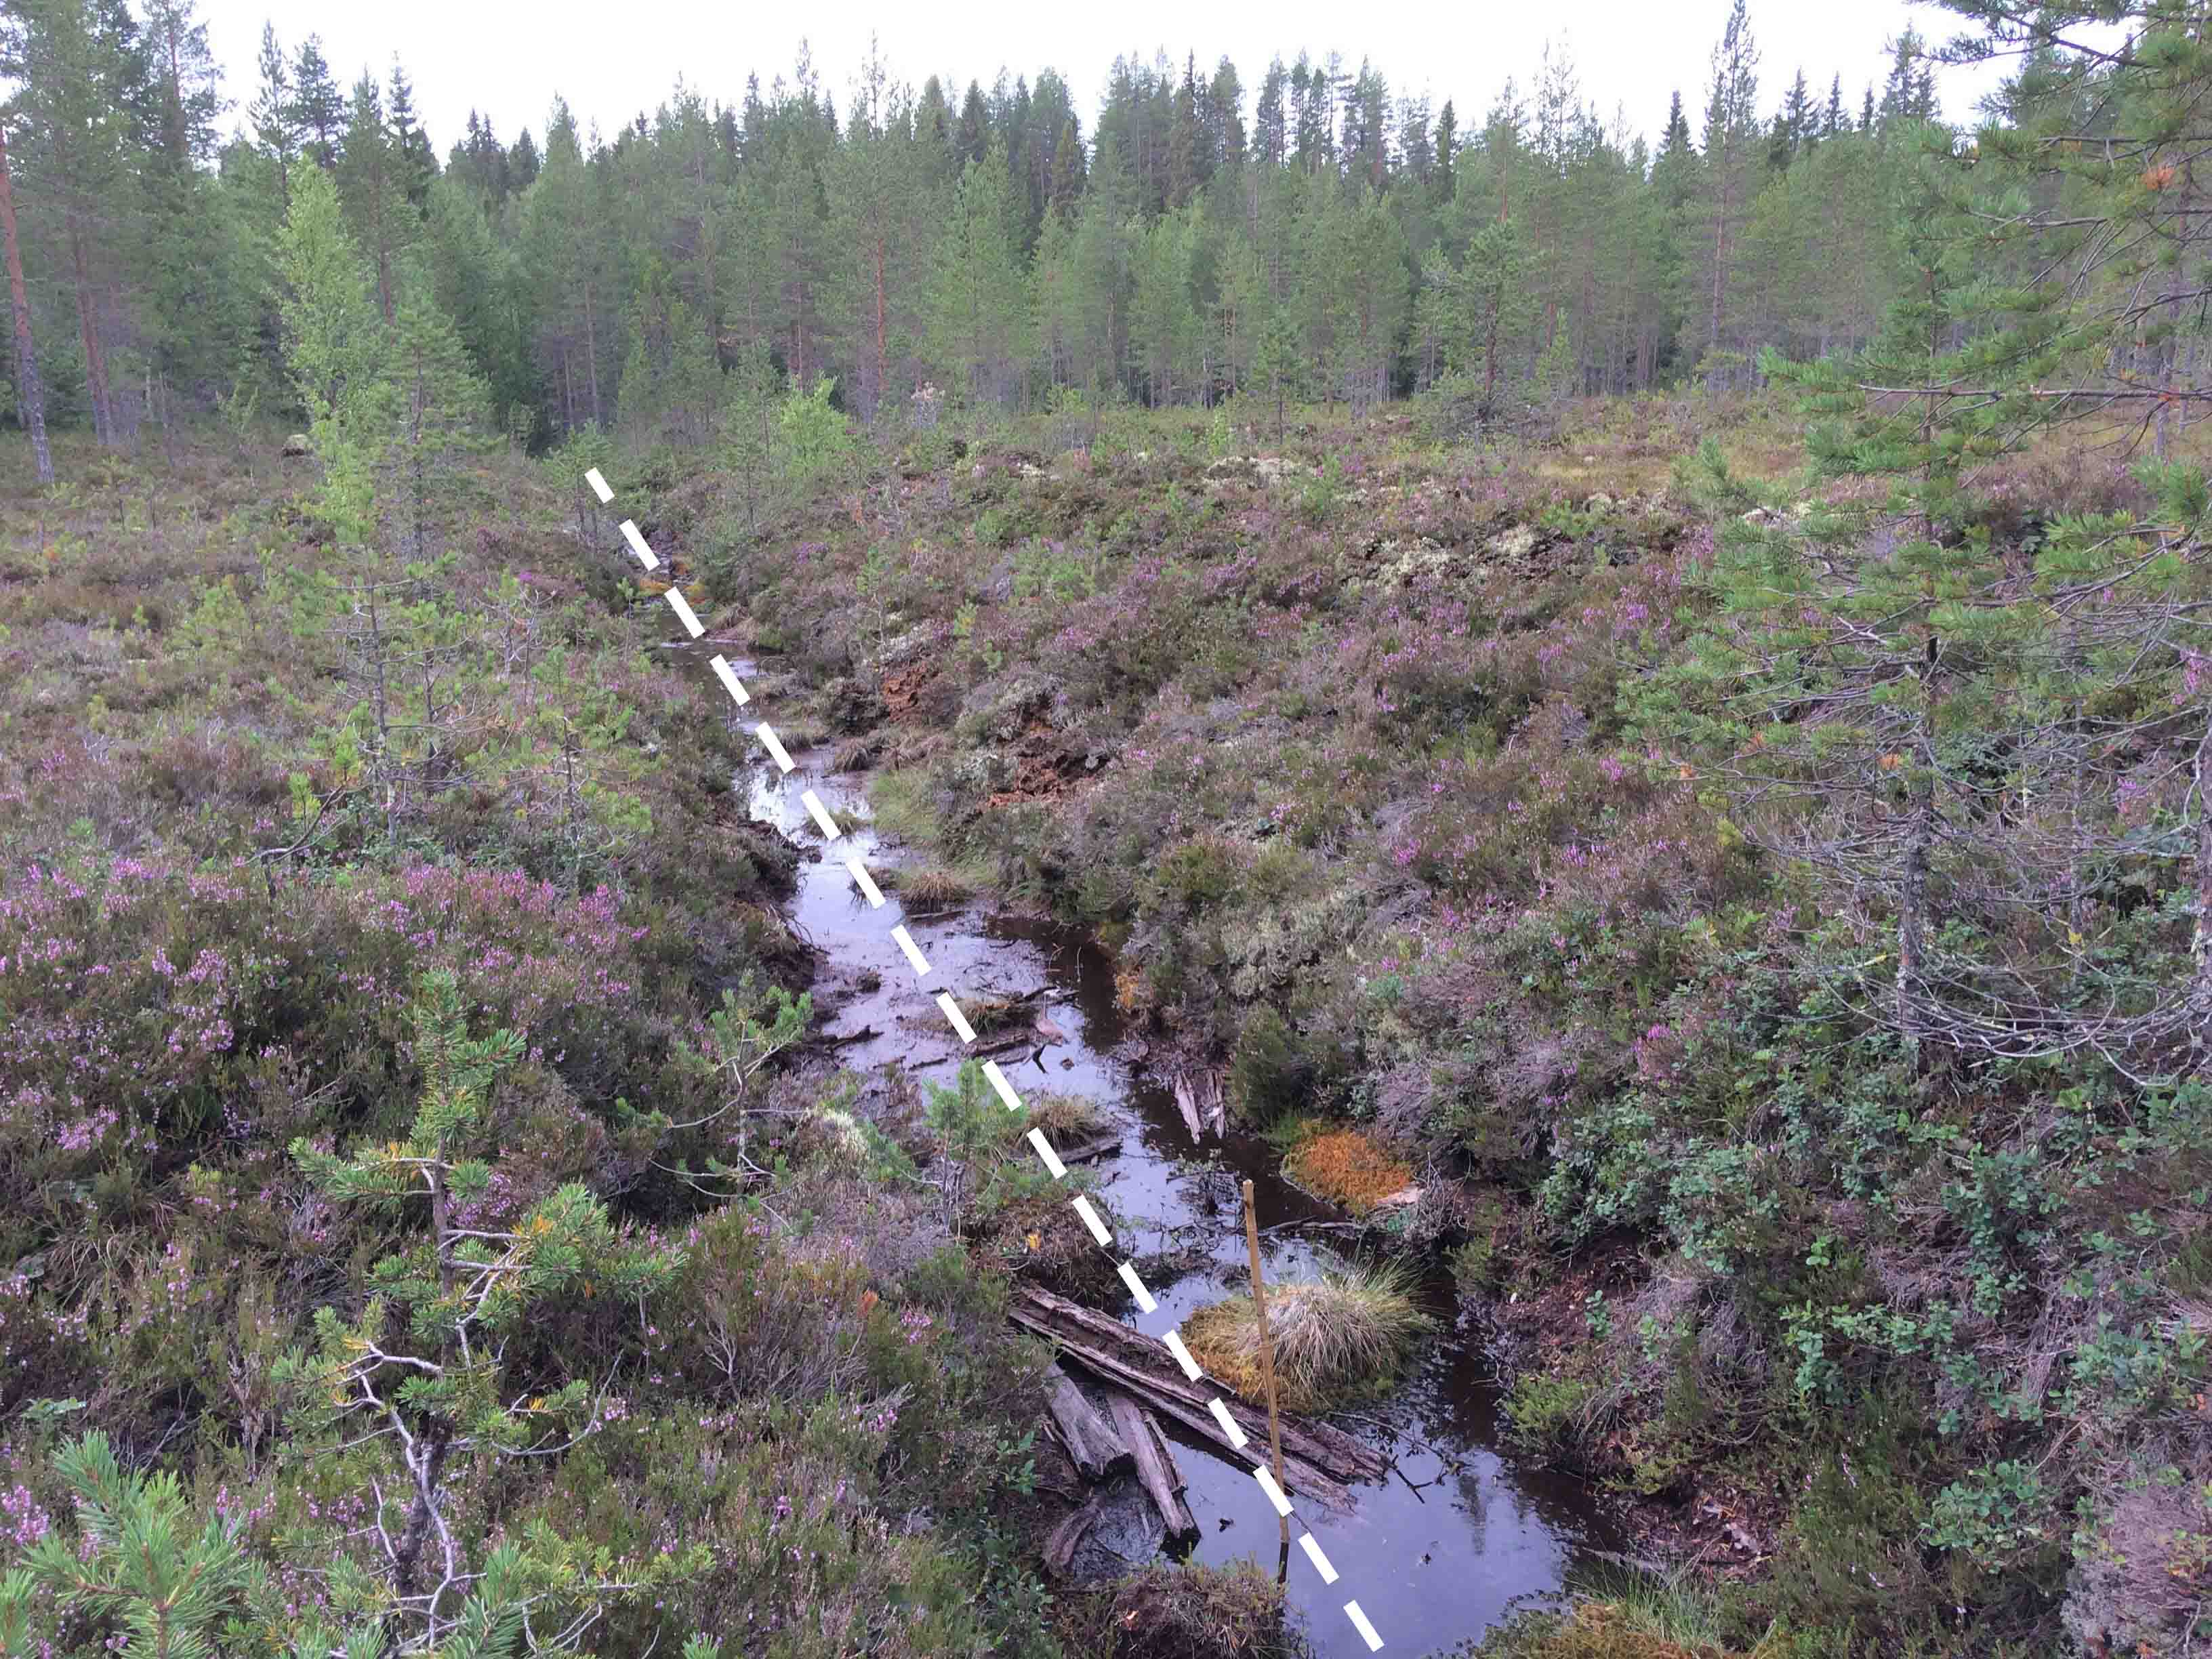
\includegraphics{./images/mire_ditch_lo.jpg}}}
    \subfigure[]{
        \resizebox*{6.8cm}{!}{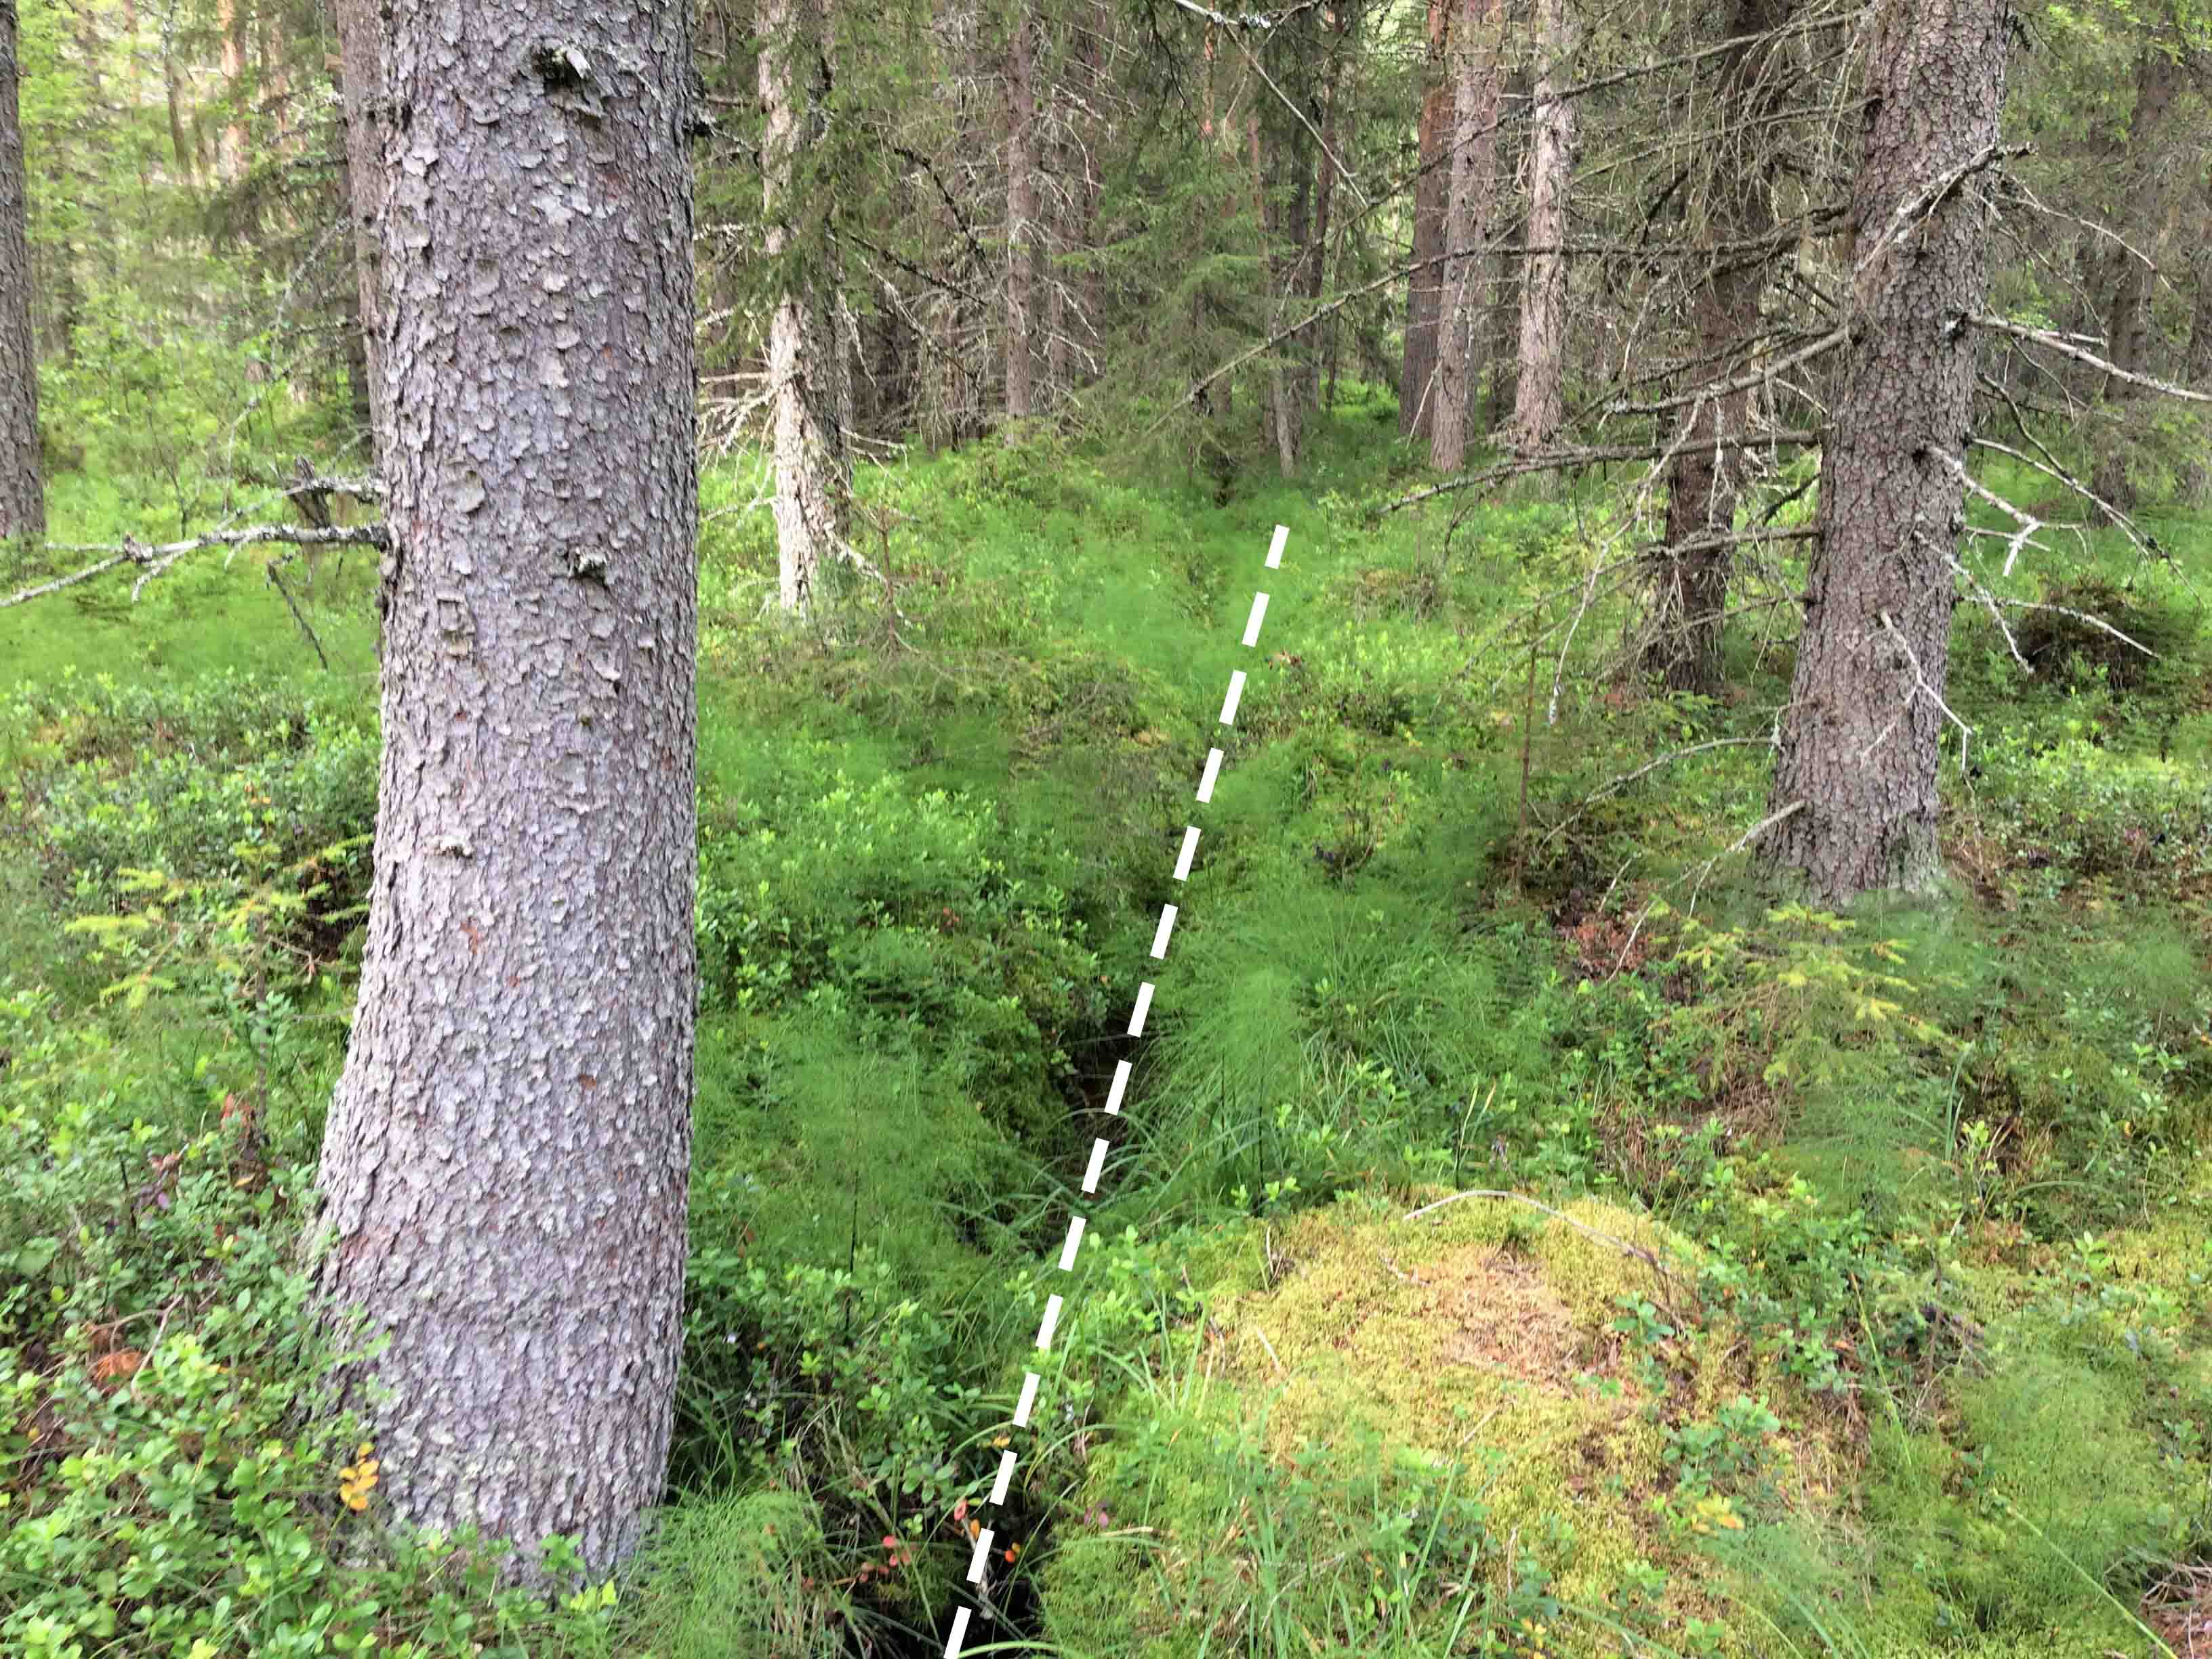
\includegraphics{./images/forest_ditch_lo.jpg}}}
    \subfigure[]{
        \resizebox*{6.8cm}{!}{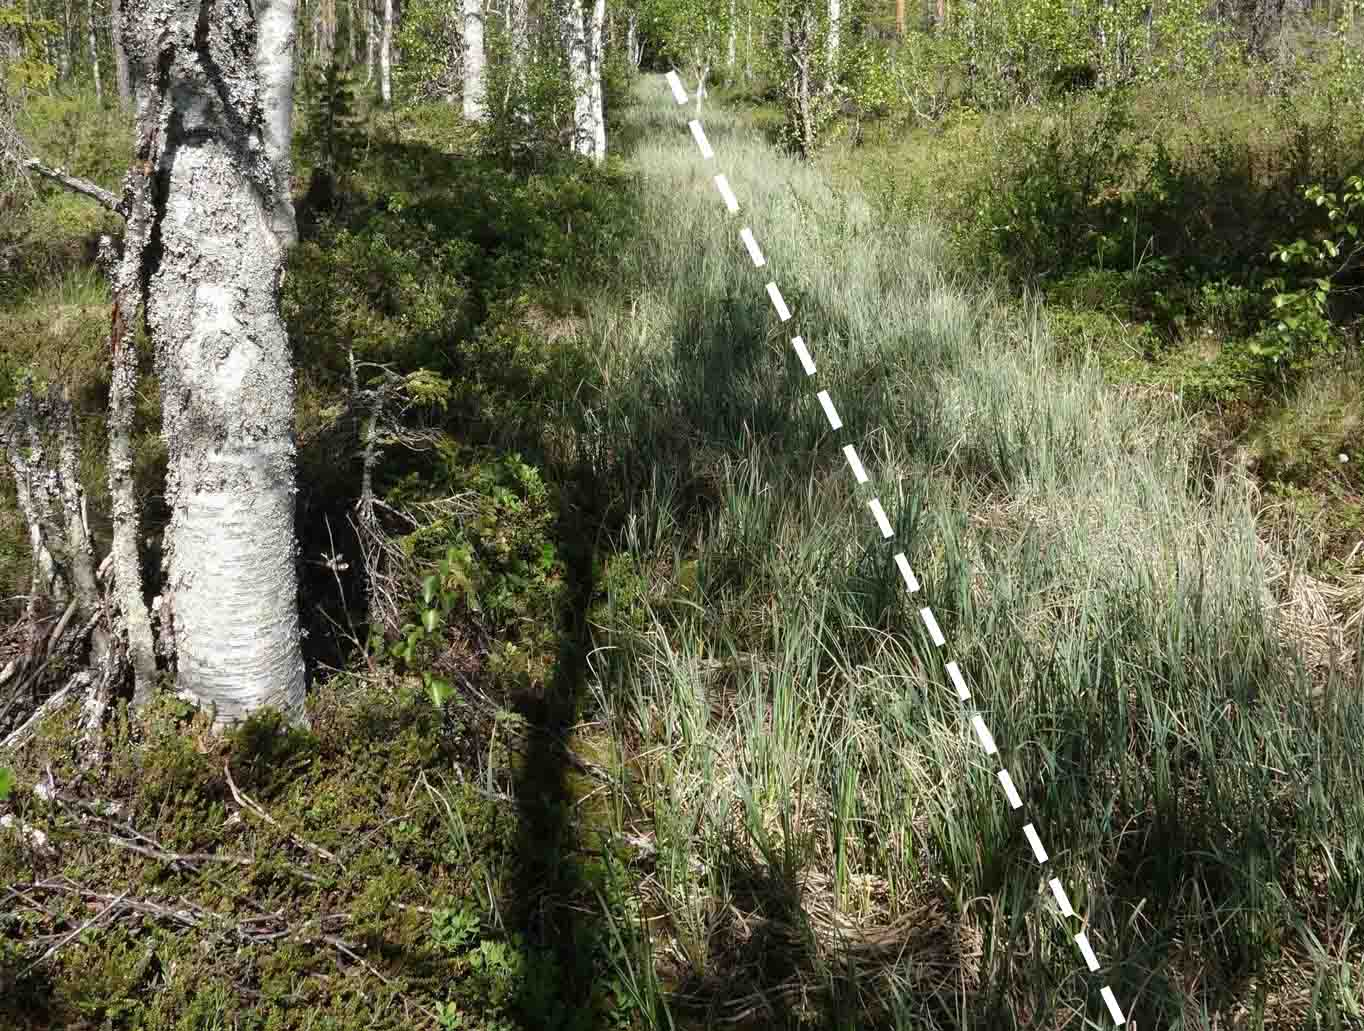
\includegraphics{./images/overgrown_ditch_lo.jpg}}}
    \caption{\textbf{Ditches in the study catchment.} These photos illustrate the difficulty of capturing the ditches based on their form (i.e. an elongated, narrow, hollow in the ground). \textbf{a: }A roadside ditch. These are generally easily detected as they are usually found in open areas along the roads, and have often been maintained. \textbf{b: }A ditch in a mire; this is still easily detected, as there is no canopy and there is a clear elevation difference between the ditch and surrounding area. \textbf{c: }A narrow, more or less  overgrown ditch in a dense forest stand. \textbf{d: }A ditch in a mire that has more or less grown back in with \textit{Sphagnum sp.} and \textit{Carex}, likely also in combination with subsiding surrounding soils. Such ditches can be found in the field as the vegetation differs, but as there is no longer an elevation difference between the ditch and the surrounding soils it will not be detected in the DEM. \newline Photos a-c: E. Maher Hasselquist, Photo d: G. Norstedt.}
    \label{fig:ditchpictures}
\end{figure}

Hypothetically, it should be quite easy to detect ditches using LiDAR data. In practice, however, there are many variables affecting the results, such as the point density and the interpolation method used to create the DEM. \citet{rapinel} found that the results were usually more sensitive to the point density (ranging 1-4 points $m^{2}$ in their study) than the interpolation method. They retrieved 54.8 and 63.8 \% of the ditches on the Aucey and Boucey marshes in France, compared to 70.28 \% in our study. However, in our study we had a LiDAR point density of 20 points $m^{2}$, so the quality of the DEM in our study ought to be robust, which may have contributed to our higher retrieval rate. \hyperref[fig:resultstreesbushes]{Figure} \ref{fig:resultstreesbushes} \hyperref[fig:resultstreesbushes]{(a, b)} illustrates the difference in the quality of the ground DEM when it is generated from LiDAR where the laser pulses have caught in trees or shrubs, and fewer points have reached the ground.

\begin{figure}[!htb]
\centering
    \subfigure[]{
        \resizebox*{5.5cm}{!}{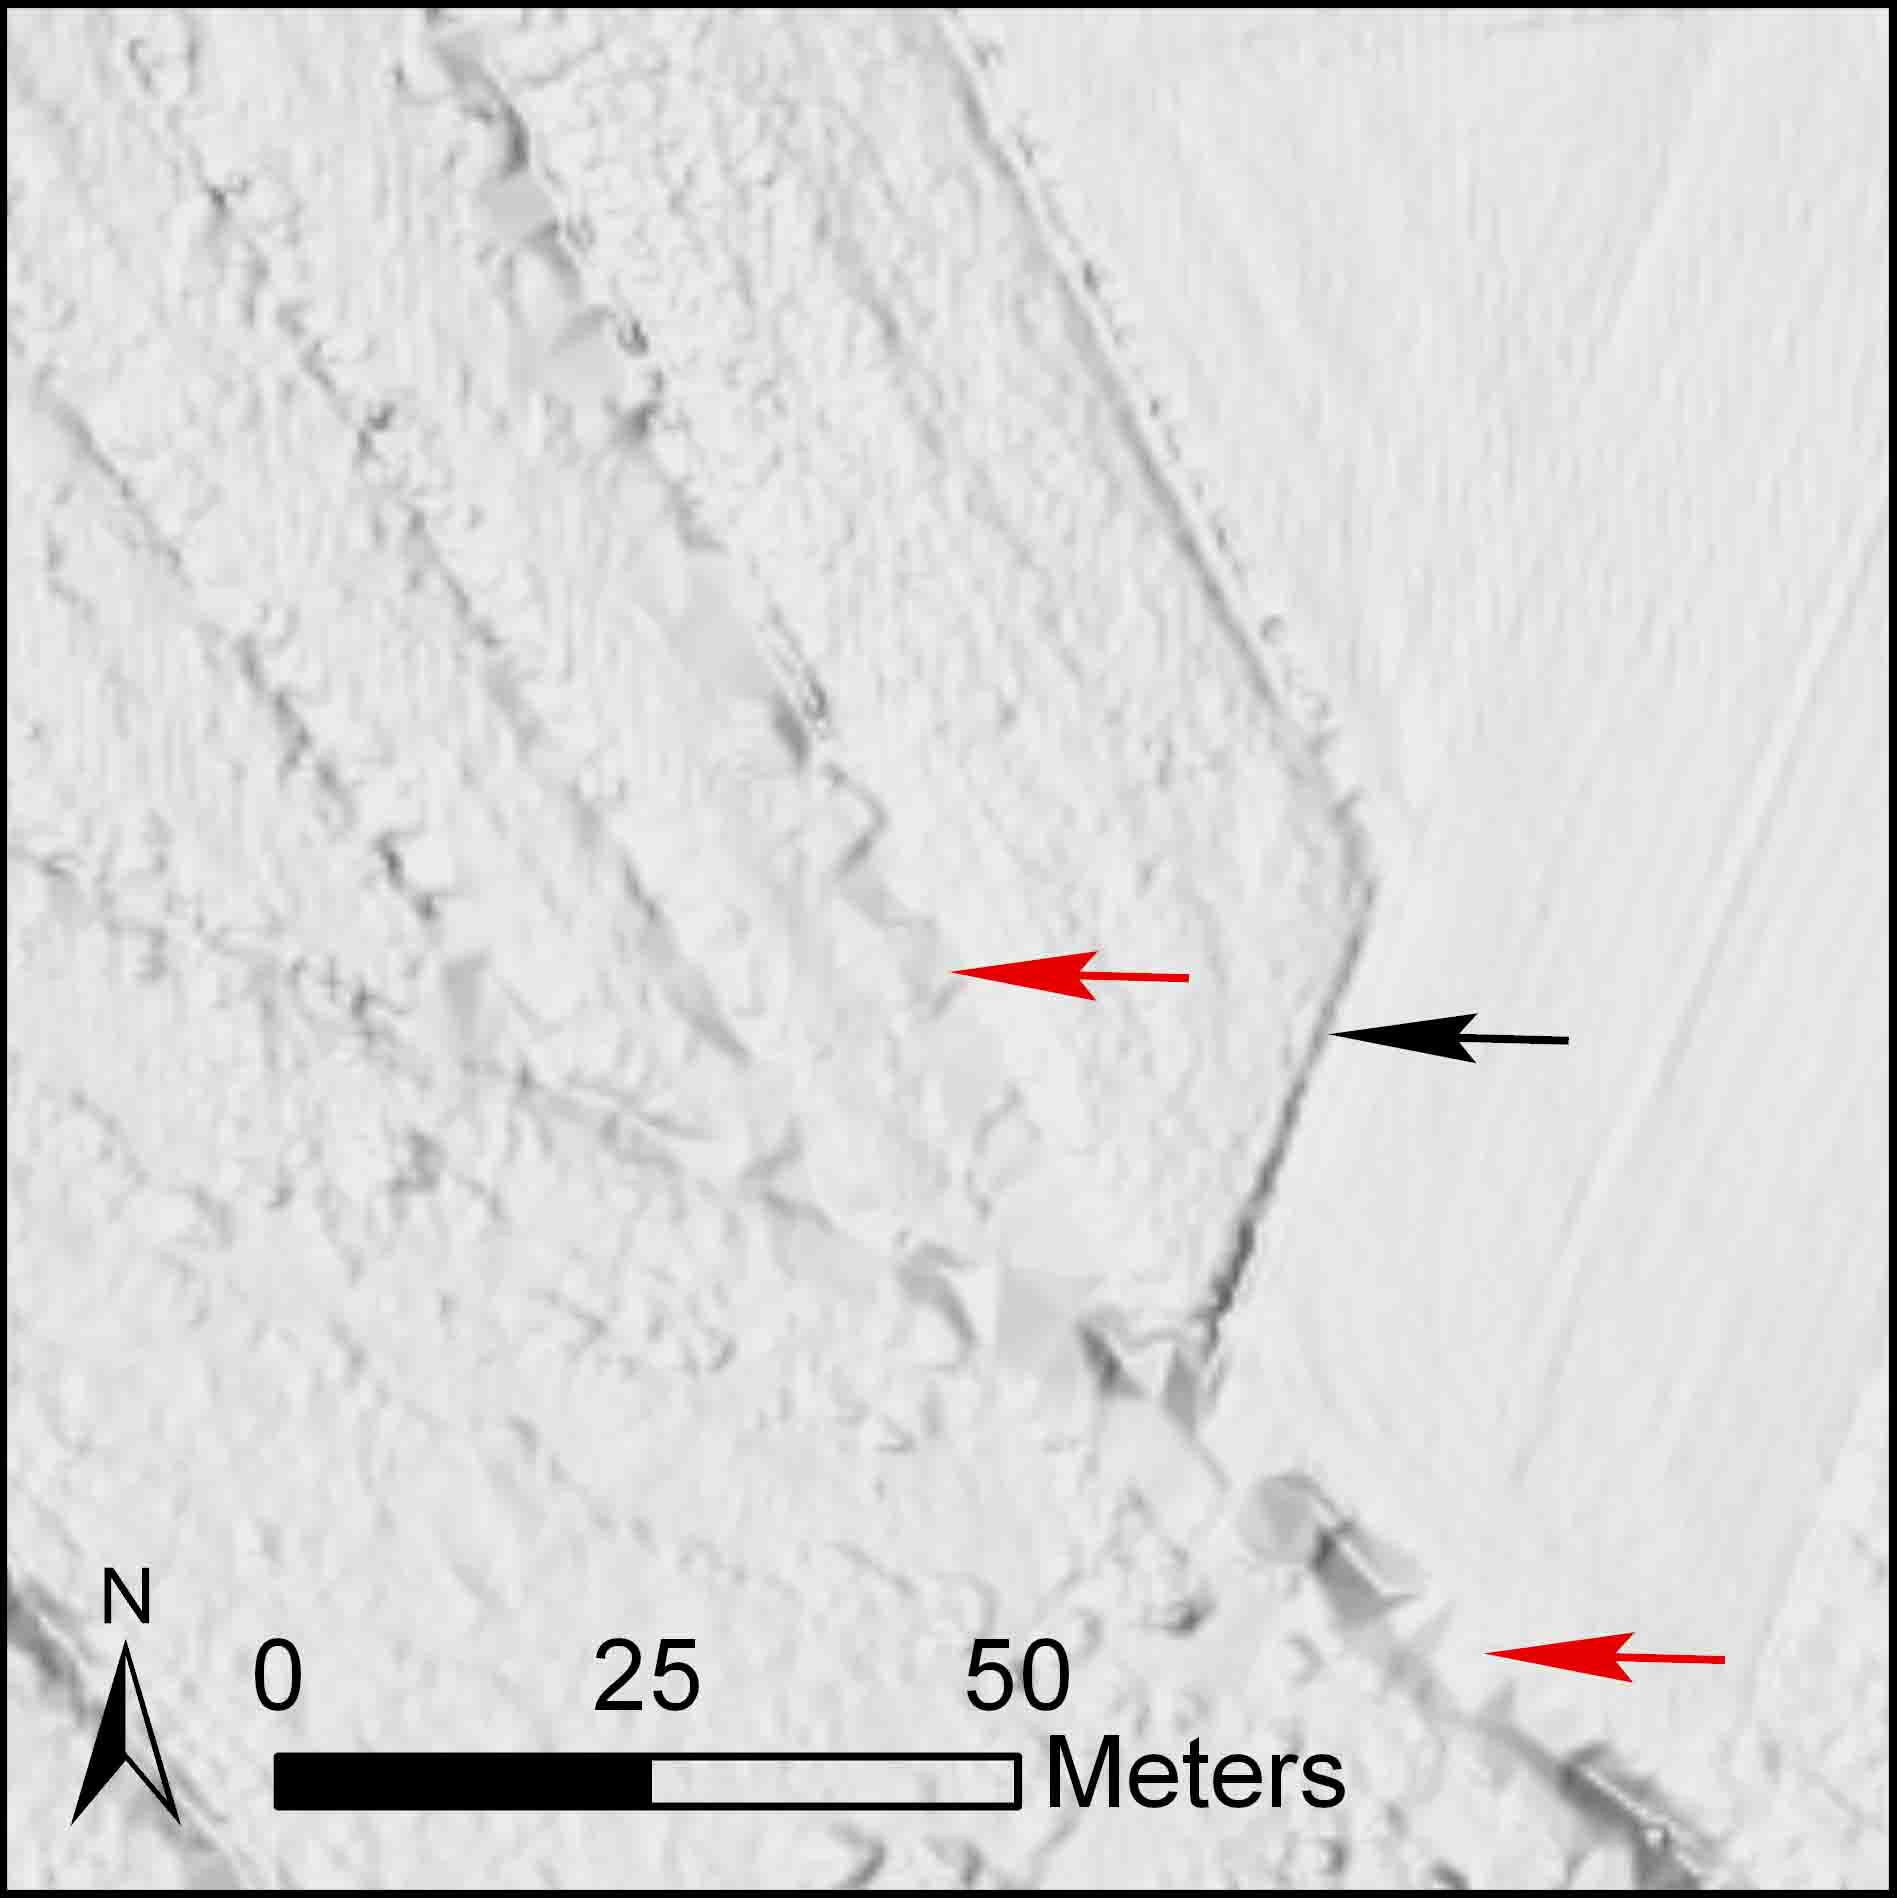
\includegraphics{./images/results_trees_bushes_1_lo.jpg}}}\hspace{7pt}
    \subfigure[]{
        \resizebox*{5.5cm}{!}{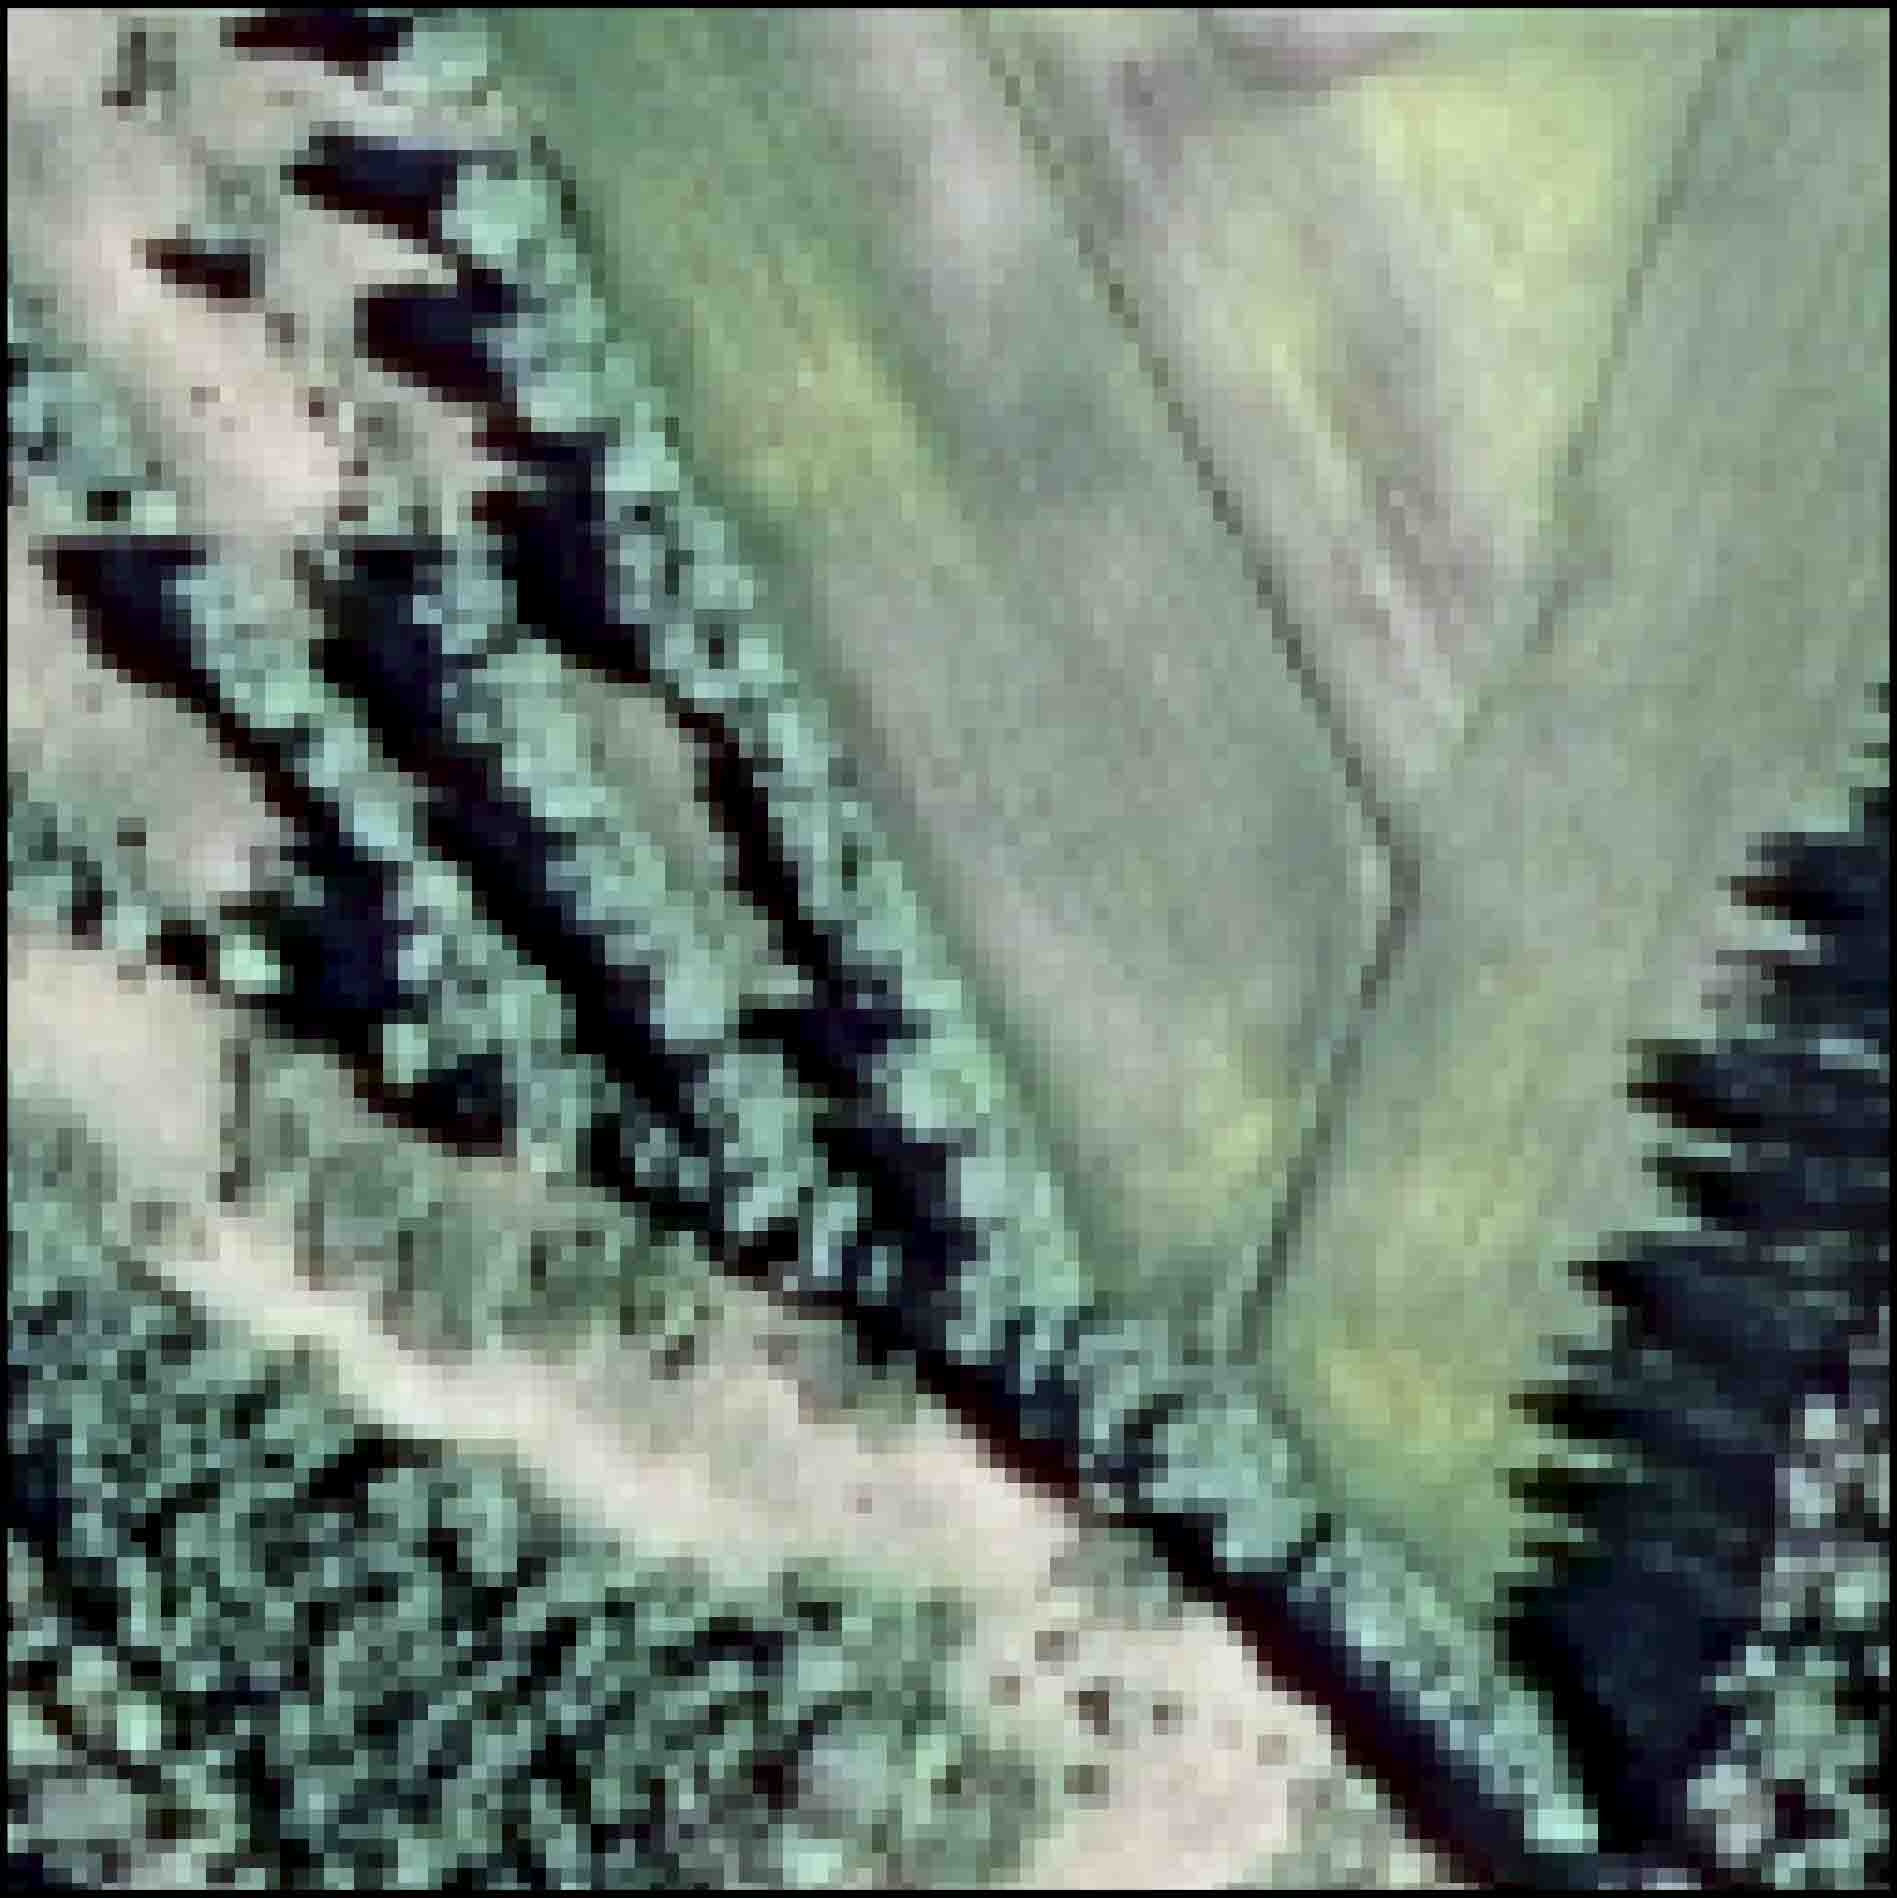
\includegraphics{./images/results_trees_bushes_2_lo.jpg}}}
    \subfigure[]{
        \resizebox*{5.5cm}{!}{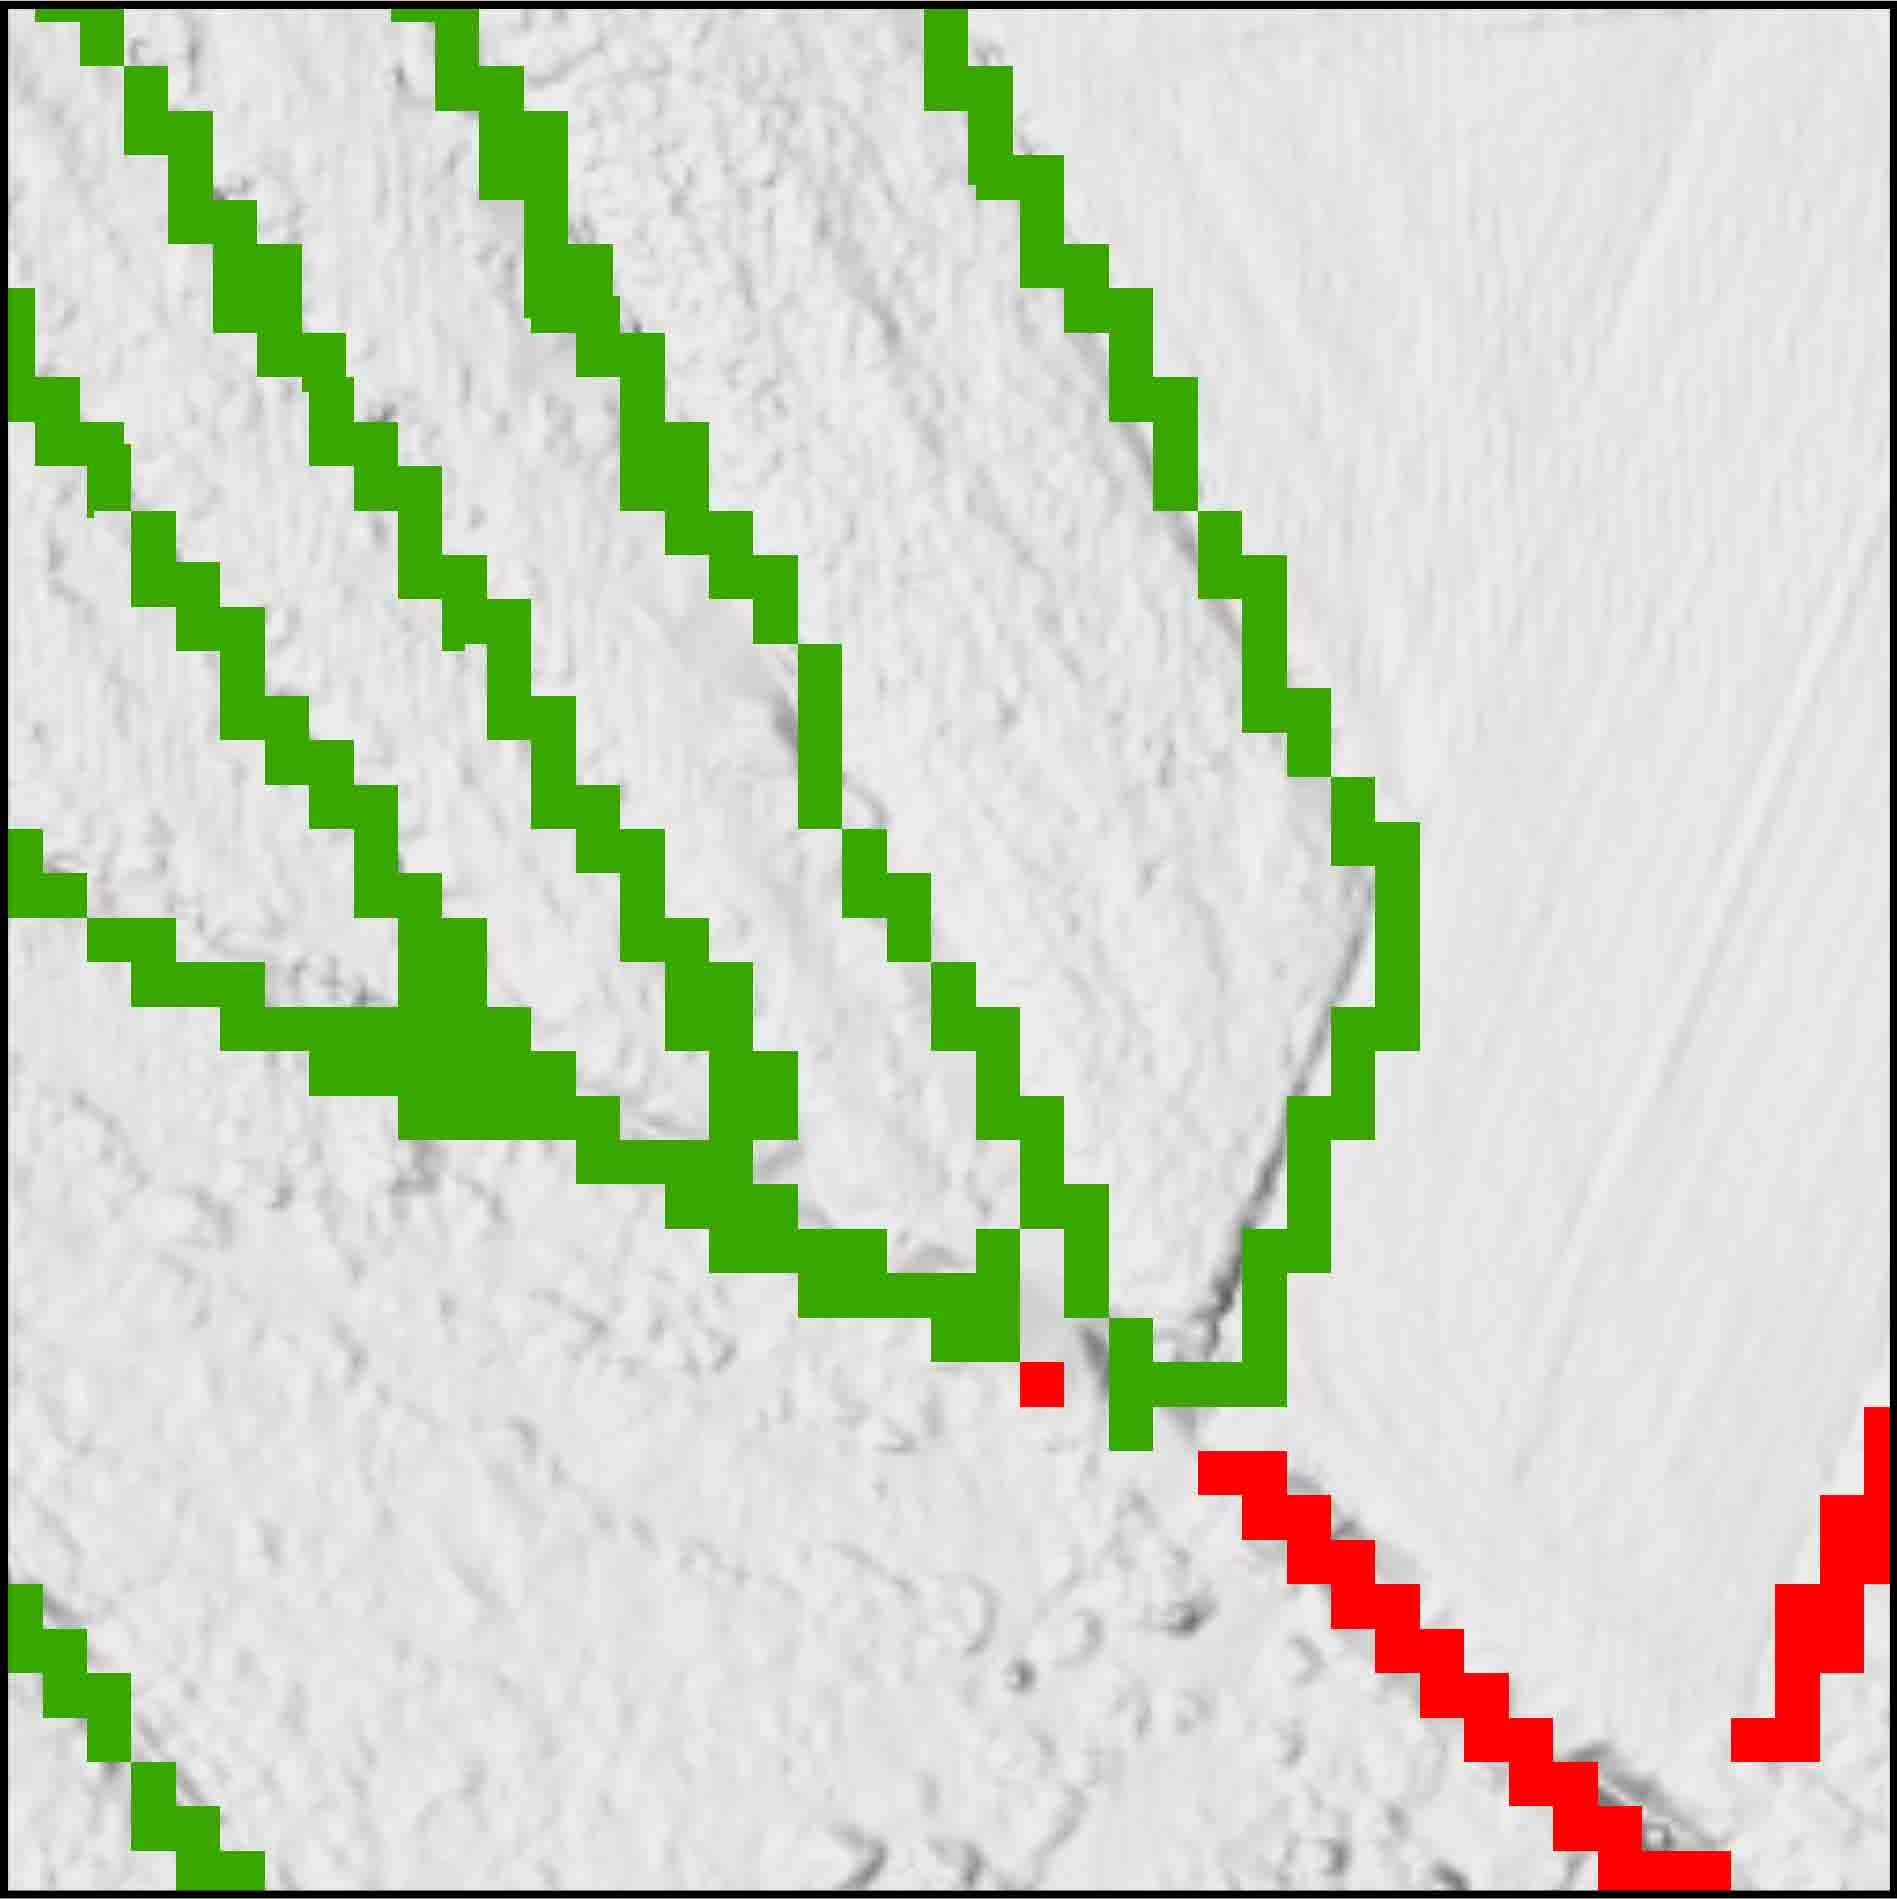
\includegraphics{./images/results_trees_bushes_3_lo.jpg}}}\hspace{7pt}
    \subfigure[]{
        \resizebox*{5.5cm}{!}{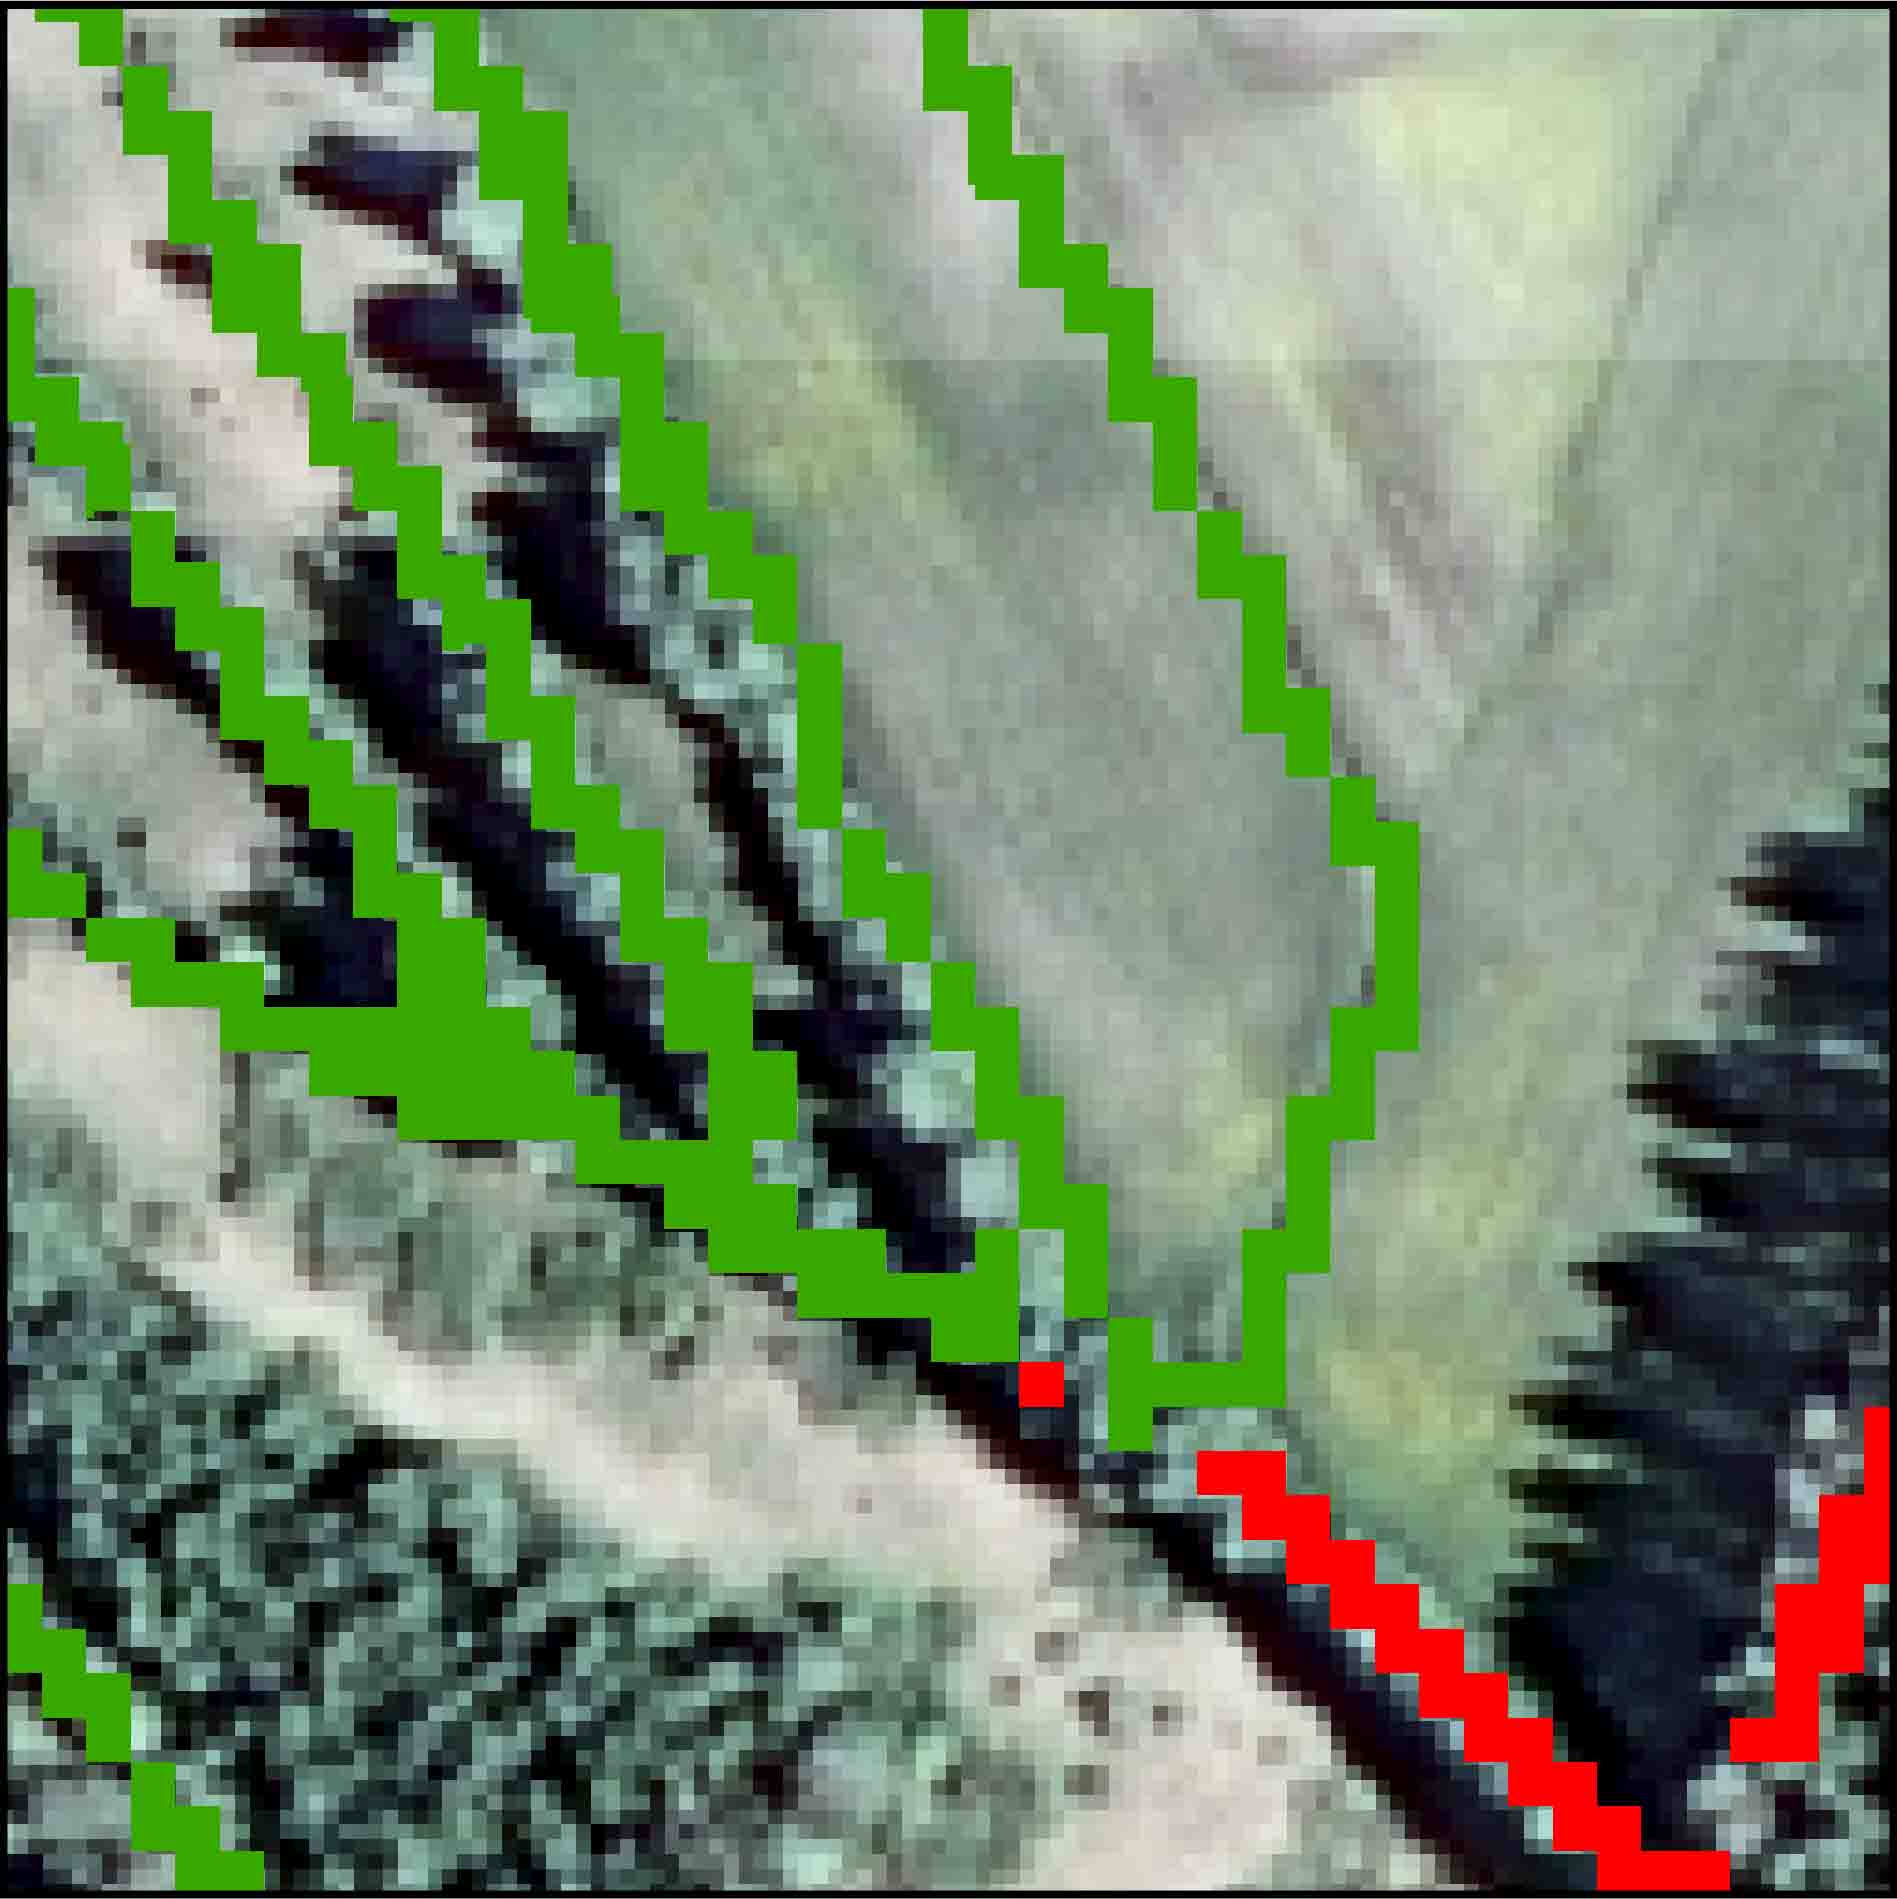
\includegraphics{./images/results_trees_bushes_4_lo.jpg}}}
    \caption{\textbf{Weak LiDAR scan illustration.} \textbf{a} and \textbf{b} illustrate that despite a LiDAR point density of 20 points $m^2$, not all points reach the ground in places with dense vegetation. In \textbf{a} there is a clear difference between the smooth surface of the DEM in the open area (black arrow), and in the areas covered by trees and shrubs (red arrows), where the DEM is much coarser due to interpolation with a lower number of LiDAR points here. The orthophoto (\textbf{b}), clearly shows that trees and shrubs are growing in the ditches in this area, making it more difficult to detect ditches. However, despite these coarser grid points in the DEM, \textbf{c} and \textbf{d} shows that the ditch detector still managed to capture a majority of the ditches (green), and only failed at certain points (red).}
    \label{fig:resultstreesbushes}
\end{figure}

A common false positive with our ditch detector is natural streams (\hyperref[fig:resultsillustrations]{Figure} \ref{fig:resultsillustrations} \hyperref[fig:resultsillustrations]{b}). However, this indicates that with some adjustments, our method could also be used to map small, previously unmapped natural stream channels. The national survey showed that 55\% of the natural stream channels and 75\% of the straightened water courses were missing on the maps (\autoref{fig:watercoursebarplot}). This is in line with other national \citep{kuglerova} and international \citep{benstead} studies highlighting this phenomenon called "Aqua Incognita - the unknown headwaters" \citep{bishop,kuglerova}.

Sometimes pixels in ditches were initially identified correctly as ditch pixels, but because not enough pixels in the surrounding area were detected, the post-processing algorithms identified them as noise and removed them. However, these steps were necessary as they helped to remove small sinks or hilly areas that had been incorrectly classified as ditches. Had we been able to use labels that were correctly labelled on a pixel basis, i.e. each ditch had its actual width recorded, the model could have learned with a better accuracy in the training phase, and the classification results would also most likely have benefitted from this. We managed to bridge gaps and exclude streams to some extent in our predictions. This was in part due to the post-processing of the predictions helping where the model was unsuccessful on its own, and in part due to the features developed.

One concern with our method is that valuable information may have been discarded when aggregating the elevations from the original point cloud to a DEM. \citet{roelens} used  machine learning to detect ditches directly from point-clouds instead of a DEM. However, we achieved a similar score to their method; $\kappa=0.73$ in our study compared to 0.77 for grassland and 0.73 for peri-urban area in \citet{roelens} study. This suggests that DEM can also be used to automatically extract ditches, provided that enough input data is available to generate a high resolution DEM for capturing the small scale features of ditches. 

\citet{bailly} also showed that the vegetation cover significantly affects the ability to detect ditches from LiDAR data (\hyperref[fig:ditchpictures]{Figure} \ref{fig:ditchpictures} \& \ref{fig:resultstreesbushes}). Approximately 75\% of the ditches in their study were retrieved where no vegetation existed, whereas the detection accuracy went below 10\% under the cover of high vegetation, shrubs, and trees \citep{bailly}. Thus, a $\kappa$ of 0.73 in our study catchment with 87\% forest cover \citep{krycklancatchment} is substantially better than that of previous research. This could possibly be a result of the higher point density of our LiDAR measurements (20 compared to 10 points per $m^{2}$). The hydrology of our study catchment also differs from that of other studies, as we have almost as many natural stream channels as ditches, whereas their studies were conducted in smaller, predominantly artificially drained areas \citep{bailly, roelens, rapinel}. Because our model locates both ditches and natural stream channels, we have to take additional measures to remove the stream channels (affecting ditch detection negatively), as explained in \hyperref[impoundmentstreamremoval]{section} \ref{impoundmentstreamremoval}.

A future improvement to the ditch detector could be to use a shape index to remove small natural streams, as natural streams often form complex channels, whereas ditches are often straight. A potential issue with generalising our ditch detector for use in other geographical areas is that many of the post-processing steps and features were developed based on occurrences in the Krycklan area. Different geographical compositions in other areas may require the adjustment of the thresholds used to fill gaps in ditches and to remove noise.

\section{Conclusion}

Detection of artificial ditches over large areas with substantial natural stream coverage is challenging, especially under tree canopy, but highly desired for effective forest management. Ditches represent elongated depressions in a DEM; however, the exact shape and size differs between ditches. We combined recently developed digital terrain indices (the most important being \hyperref[impoundment]{Impoundment} Index and High Pass Medium Filter) but, unlike previous studies, did not apply generic thresholding on them. Instead, we included local variability in the indices by using different radii to capture ditches with varied shapes. This integration of a large set of terrain indices using machine learning produced good results, as evidenced by the confidence interval for the Cohen's $\kappa$ index, which ranged from 0.655 to 0.781 with a confidence level of 95\%. With the developed features and extensive post-processing, we also managed to remove many stream channels and fill gaps in the ditches where the LiDAR scans were weak. 

Although there is room for further improvement, the methodology is a significant step forward as it performed on a par with previous studies conducted in more homogeneous agricultural landscapes. Our approach enables accurate ditch detection in complex forested landscapes with tree canopy and many natural streams. Future work could introduce more features and post-processing steps, such as using pathfinding algorithms to fill gaps in the ditch model or shape indices to remove stream channels from the prediction. Moving towards image segmentation instead of pixel classification of tabular pixel values could also be a suitable future approach. Our developed methodology can be adjusted to apply to any setting for artificial ditch detection, reducing time and labour investment compared to the conventional manual mapping techniques. The accurate ditch maps can both significantly contribute to practical forestry and operational land management, as well as allow government agencies, forest companies, and regional and local authorities to predict the climate consequences of potential management actions, which will be critical in reaching global sustainability goals.

\section*{CRediT authorship contribution statement}

\hl{ Jag tolkar det som att denna sektion \"ar frivillig, men ESWA skriver i guiden att de uppmuntrar att man fyller i denna. De flesta artiklar jag har hittat listar h\"ar vad alla enskilda f\"orfattare har bidragit med. Kategorier: Conceptualization; Data curation; Formal analysis; Funding acquisition; Investigation; Methodology; Project administration; Resources; Software; Supervision; Validation; Visualization; Roles/Writing - original draft; Writing - review & editing.}

\section*{Declaration of Competing Interest}

The authors declare that they have no known competing financial interests or personal relationships that could have appeared to influence the work reported in this paper.

\section*{Acknowledgements}
We wish to thank Dr. Siddhartho Paul at the Swedish University of Agricultural Sciences, whose suggestions helped improve and clarify this manuscript. We also thank Sigurd Israelsson at the School of Engineering at J\"onk\"oping University for lending hardware resources for the experiments in this study. This work was supported by VINNOVA, EU InterReg Baltic Sea project WAMBAF tools and Formas. \hl{ H\"ar ska varje grant definieras med "grant number[xxxx] efter varje akt\"or", jag tolkar det ocks\aa som att man ska skriva vilken roll varje finansi\"ar har.}


\bibliography{references}

\end{document}
